% !TEX TS-program = xelatex
% !TEX encoding = UTF-8 Unicode
% this template is specifically designed to be typeset with XeLaTeX;
% it will not work with other engines, such as pdfLaTeX

%%% Count out columns for fixed-width source font
% 000000011111111112222222222333333333344444444445555555555666666666677777777778
% 345678901234567890123456789012345678901234567890123456789012345678901234567890

\setheaders{\shorttitle{} Liber I}{\shortauthor{}}
\chapter{Liber Primus - De anno aequabili minore}
\begin{center}
{\scshape
IOSEPHI SCALIGERI IULII CAESARIS F.\\
DE EMENDATIONE TEMPORUM\\
LIBER PRIMUS\\
}% scshape
\end{center}
\normalsize

% 1
% {PDF page nr}{source page nr}{line nr}
\plnr{84}{1}{1}Si verum est, quod sciscit Stoicorum
schola, Tempus esse normam rerum, et
custodiam, quia veritatis index atque examen
est, et rerum gestarum memoriam, ac
diuturnitatem posteritati tuetur: ii non vulgari
laude digni sunt, qui temporum rationes
conscribere, atque fugitivam antiquitatem
retrahere conantur.
\lnr{8}Qua in re cum
tam priscis scriptoribus, quam aequalibus
temporum nostrum opera egregie navata sit, dolendum tamen, aut
ferius, quam oportebat, antiquos sese ad id studium contulisse, aut pauciora
ea de re monumenta, quam ab ipsis auctoribus relicta sunt, ad
nos pervenisse.
\lnr{13}Nam ut omnia extent veterum Graecorum scripta, ea
tamen paucorum temporum intervallum complectebantur.
\lnr{14}Graecis
enim ante initia Olymiadum suarum nihil plane exploratum est: et,
quod dolendum est, de illorum scriptis, quae ad Chronologiam spectabant,
nihil nobis praeter desiderium relictum est.
\lnr{17}Nam quae Eusebii exstant,
quamuis ex Graecorum monumentis hausta sunt, et multa egregia
% è -> ex
ac cognitu digna nobis conservarunt: tamen dissimulandum non est,
multa in illis reperiri, quae castigatioribus iudiciis non satisfaciant.
\lnr{21}Quod si Thalli, Castoris, Phlegontis,
 Eratosthenis canones exstarent,
perparua, aut nulla potius ratio haberetur librorum quorundam, qui
hodie in penuria meliorum nobis in pretio sunt.
\lnr{23}Apud Romanos vero,
ea scriptio infeliciter cessit, quod eam cognitionem ferius amplexi sint.
\lnr{25}Nam ante Consulatum Bruti nihil certi apud illos: omnia fabulosa: et,
si rem propius spectemus, ne ipsius quidem Bruti Consulatum, ac tempus
Regifugii satis exploratum habent.
\lnr{27}Quamuis, ut prodidit Censorinus,
Varro collatis diversarum civitatum temporibus, et intervalla retexens,
verum in lucem protulerit, et viam reperit, qua certus
annorum Urbis conditae numerus iniri posset.

% 2
% {PDF page nr}{source page nr}{line nr}
\plnr{85}{2}{2}Sed, ut suo loco disputabitur,
non magis constabat Varroni de initiis Urbis, quam Graecis de
anno excidii Troiae.
\lnr{4}Nam ea demum est vera demonstratio, quae cogit,
non quae persuadet.
\lnr{5}Soli sacri libri supersunt, ex quorum fontibus
certa temporum ratio hauriri possit.
\lnr{6}Sed omnis temporum cognitio
inutilis est, nisi certa epocha in illis deprehendatur, ad quam omnium
temporum contextus, tam antecedentium, quam consequentium referri
possit.
\lnr{9}Nam, ut praeclare dixit vetus inter Christianos scriptor
Tatianus, apud quos temporum notatio non cohaeret, apud illos neque
veritatis et fidei historicae ratio ulla constare potest.
\lnr{11}Quod si aliquis
sacrae historiae peritissimus, hoc est, qui intervalla rerum gestarum
nobilissima certissimis ratiociniis ex Mose, et
 reliquis sacris Bibliis explorata
habeat, nihil tamen ex illis ad certam epocham historiae Graecae,
aut Romanae referre possit: quodnam adiumentum is ex eiusmodi
diligentia adferre potest aut sibi, aut studiosis rerum antiquarum?
\lnr{17}Nam omnis cognitionis finis ad usum aliquem spectat, quem si ex medio
literarum sustuleris, ingratus est omnis labor et opera, quaecunque
in omne studium impenditur.
\lnr{19}Eiusmodi est Iudaeorum scientia, qui
in ratiociniis quidem sacrorum temporum colligendis tantum studio
et diligentia consecuti sunt, ut proxime ad veritate abesse dici possint: sed
% à -> ad
dum nullam aut saltem depravatam rerum extrarum cognitionem
tenent, multum errant, quod sine externa historia sacram tractare
aggrediuntur.
\lnr{24}Venio ad nostros, recentiores dico, qui hodie summo
cum fructu, sacrae, Graecae, et Romanae historiae tempora digesserunt.
\lnr{26}Ii heroica virtute chronologiam negligentia et contemtu maiorum
intermortuam ac sepultam, ex tenebris et oblivionis silentio quotidie
% è -> ex
eruere conantur.
\lnr{28}Certe meum semper iudicium fuit, eam rem maiore
cum laude ab illis restitutam, quam ab antiquis proditam fuisse.
\lnr{29}Nam
non solum pleraque in ratione temporum pristinae integritati reddiderunt,
sed et longe meliora effecerunt.
\lnr{31}In multis tamen iudicium, in quibusdam
etiam diligentiam requiro.
\lnr{32}Neque enim dum verum adepti sunt.
\lnr{33}Argumento suerint omnium, quotquot de his rebus tractarunt,
 dissensiones:
ut inter tot millia Chronologorum vix inter duos de eadem re
conveniat.
\lnr{35}Quanta adhuc contentione de Septimanis Danielis, de initio,
medio, et fine earum velitantur?
\lnr{36}Tamen nihil plane eorum, quae volunt,
assecuti sunt.
\lnr{37}Ab eorum lectione incertior atque indoctior sum,
quam dudum.
\lnr{38}Quis unquam eorum veram epocham Exodi Habraeorum;
quis, quod pudendum est, verum annum natalis Dominici odoratus
est?
\lnr{40}Ecce trita, obvia, vulgaria, ut nobis videtur, ignoramus, et remotiorum
ac reconditiorum indicium promittimus!
\lnr{41}Quis eorum Danielis
Hebdomadas interpretandas suscepit, qui inscitiae suae latebram
non quaesiverit, et reges Persidis, qui nunquam in rerum natura fuerunt,
non commentus sit?

% 3
% {PDF page nr}{source page nr}{line nr}
\plnr{86}{3}{3}Quod si Danielem accuratissime legissent,
eis ad negotium explicandum non aliis regibus Persidis opus fuisset,
quam iis, quos Herodotus, Diodorus, et omnis Graecorum antiquitas
novit.
\lnr{6}Sed quo non progressa est \textgreek{[Greek]}?
\lnr{6}Berosos, Metasthenes, et
nescio quos Catones, ac Philones consulunt, qui ante hos centum annos
ex officina nescio cuius indocti et impudentis prodierunt.
\lnr{8}Et sese
Criticos in temporum notatione profitentur, quibus tam facili genere,
tam pueriliter unus homo otiosus in tanta luce literarum quotidie imoponit.
\lnr{11}Cuius hominis inscitiam si nihil aliud, certe illud arguere
 possit, quod
Metasthenem pro Megasthene posuit.
\lnr{12}Si Iosephum Graece, aut Strabonem,
aut Athenaeum legisset, is Megasthenem vocari deprehendisset,
quem Metasthenem vocat.
\lnr{14}Si Graece scisset, nunquam \textgreek{[Greek]} in illa
lingua reperiri, neque hanc compositionem in eadem probari intellexisset.
\lnr{16}Ut igitur ii resipiscant, qui et novos reges in Perside crearunt,
et Assueros Priscos, Assueros Longimanos, Assueros Pios, duos Cyros,
et nescio quae alia somnia Annii Viterbiensis in medium producunt,
primum uno verbo indicabo fontem erroris eorum: deinde qui medicina
huic morbo fieri possit, docebo.
\lnr{20}Quod igitur in veri investigatione
eos ratio fugerit, duas summas causas reperio: unam, quod veterum
tempora civilia, annorum, mensium formas, status, ac genera ignorarunt:
alteram, quod characterem, et notationem ei anno, quem sibi
proposuerant, non adhibuerunt.
\lnr{24}Ex utraque quidem causa temporum
confusio manavit, sed diverso genere.
\lnr{25}Ex priore causa ignoratus est
annus, mensis et dies multarum nobilium epocharum.
\lnr{26}Huius enim
rei cognitio pertinet ad tempus civile nationum.
\lnr{27}Ex altera causa Palilia
urbis Romae nunc tertio anno Olympiadis, nunc quarto attribuuntur.
\lnr{29}Item Consulatus Bruti nunc in hunc, nunc in illum annum
Olympiadis confertur.
\lnr{30}
Ut igitur novam rationem emendationis temporum
ineamus, duo illa praecipue nobis discutienda sunt: sed prius
de omnium nationum temporibus civilibus: quam assequi perdifficile
est, nisi prius tempore in sua principia, hoc est ab annis, periodis,
mensibus in ultimum terminum, dies, horas ac scrupula resoluto.
\lnr{35}Nam qui ante nos hanc provinciam aggressi sunt, si modo hanc nostram,
non aliam aggressi sunt, ii satis de tempore, et eius natura
disputarunt.
\lnr{37}Sed hanc disputationem melius interpres \textgreek{[Greek]}
sibi vindicasset.
\lnr{38}Neque vero nos id agimus, ut difiniamus
tempus esse hoc secundum Peripateticos, aut illud secundum Stoicos,
aut Academicos.
\lnr{40}Qui istis definitionibus diu immorati sunt, et hac
sola scientia Chronologiae scribendae modum terminarunt, illi fatis
verborum quiedem, sed rerum nihil definiverunt.

% 4
% {PDF page nr}{source page nr}{line nr}
\plnr{87}{4}{1}Nequid tamen
\textgreek{[Greek]} transigatur, decrevi singularum, vel
 minimarum temporis
partium prius conspectum aliquem dare, quam ad descriptionem
\textgreek{[Greek]} temporum civilium, et eorum methodum aggrediar.
\lnr{4}Incipiam igitur ab ultimo termino, a die scilicet, et eius partibus,
hoc est hora, et scrupulis.
\lnr{6}Ab hora igitur, si libet, principium esto.

\section{De Horis et partibus diei reliquis}

\lnr{7}Veteribus statim ab initio has diei partes, quas \textsc{Horas}
vocamus, in usu non fuisse, argumento fuerint priscae locutiones,
quibus dies non in partes secatur, sed actionibus quotidianis
distiguitur: ut cum \textgreek{[Greek]} vesperam vocabant, 
nimirum, ut poëta
% Source: poëta; Rare occurence of a diaeresis. Not sure if it should be
% left there or removed.
inquit, \textit{Demeret emeritis cum iuga Phoebus equis}.
\lnr{11}Item quod tempus
antemeridianum disignantes dicebant \textgreek{[Greek]}
 vel \textgreek{[Greek]},
convenientibus scilicet eo tempore in Comitium viris: ut Hesiodus dicit,
\textgreek{[Greek]}.
\lnr{14}Quod tamen longe aliter interpretes
Graeci illius poëtae exponunt.
% Source: poëtae
\lnr{15}Aiunt enim Hesiodum intellexisse
de tricesima mensis Lunaris: et sensum loci Hesiodei esse perinde
ac si dixisset, Quando homines veram \textgreek{[Greek]} Lunarem agunt, et
non secundum usum politicum, sed secundum motum Lunae.
\lnr{18}Quod
tamen nobis valde coactum videtur: et mentem Hesiodi hanc fuisse dicimus:
\textgreek{[Greek]} esse valde idoneam rebus gerendis ea hora,
 qua homines
ad ius in forum conveniunt.
\lnr{21}
Homerus Odyss. \textgreek{[Greek]}
% Expand "Odyss." in the propper way, with the correct declension.
\begin{quote}
\textgreek{[Greek]}\\
\textgreek{[Greek]}
\end{quote}

\lnr{24}Quae sane interpretatio melior vulgari.
\lnr{24}Sic etiam paulo post dicit,
\textgreek{[Greek]}, loquens de undecima: cuius partem designat,
 cum dicit
\textgreek{[Greek]}.
\lnr{26}Quod nos interpretamur iam adulto die.
\lnr{26}Sic Homerus
meridiem designat, \textgreek{[Greek]}.
\lnr{27}Porro neque
hoc verbum \textgreek{[Greek]} id, quod nunc, valebat.
\lnr{28}Sed tempus actuum quotidianorum
illo notabatur: ut cum dicebant \textgreek{[Greek]}.
\lnr{29}Latinis
vero Tempestas dicebatur.
\lnr{30}In Legibus Decemvirum Atticis fuit:
\textsc{Sol occasus suprema tempestas esto}.
\lnr{31}Neque recte
quidam hinc expungunt \textsc{tempestas}.
\lnr{32}Quod \textsc{suprema} absolute
diceretur, ut apud Plautum.
\lnr{33}Nam plane in legibus Solonis, unde illud
caput traductum, scriptum fuit,
 \textgreek{[Greek]}.
\lnr{34}Stoicus
scriptor apud Stobaeum loquens de Socratis iudicio capitali: 
\textgreek{[Greek], [Greek], [Greek]
ΕΣΧΑΤΗΝ ΩΡΑΝ [Greek], [Greek] ΗΛΙΟΣ ΕΠΙ ΤΩΝ
ΟΡΩΝ, [Greek]}.
\lnr{38}Idem censeas de veteribus Hebraeis,
qui diei nullas alias partes, quam mane, meridiem, et vesperam norant.
et ita dies dividitur Psalmo \rnum{lv}, commate \rnum{xviii}.
% Psalm 55:17 (KJV) "Evening (εσπέρας), and morning (πρωϊ),
% and at noon (μεσημβρίας), will I pray, and cry aloud:
% and he shall hear my voice."

% 5
% {PDF page nr}{source page nr}{line nr}
\plnr{88}{5}{2}Sic Homero,
\textgreek{[Greek]}.
\lnr{3}Sed hic dies intelligitur Lux, exclusa nocte.
\lnr{4}Nam totum \textgreek{[Greek]} Hebraei in quatuor partes
 dividebant, quas vigilias
vocabant.
\lnr{5}Prima vigilia erat ab vespere: secunda ab media nocte:
tertia ab mane: quarta ab meridie.
% à -> ab (4x)
\lnr{6}Alioqui nomen hoc \texthebrew{[Hebrew]} quo hodie
horam designant, ne notum quidem illis erat: atque apud Danielem
aliud significat.
\lnr{8}Posterorum inventum est Horologium, et \textgreek{ηλιοτρόπια},
%[Greek: heliotropia; probably: sundails]
quibus dies per lineas, et intervalla umbrarum distinguebatur.
\lnr{10}
Unde prodiit locutio \textgreek{[Greek]}, pro hora coenae.
\lnr{10}Vel \textgreek{[Greek]}:
quia notis literarum singularium horae distinguebantur.
\lnr{11}Testatur et Epigrammatium de Horologio:
\begin{quote}
\textgreek{[Greek]}\\
\textgreek{[Greek]}
\end{quote}
\lnr{14}Nam ante
\textgreek{Ζ, Η, Θ, Ι,} erat \textgreek{Α, Β, Γ, Δ, Ε, ς.}
\lnr{15}Arabibus, Persis, et reliquis Orientis
gentibus non horologiis, sed
naturalibus matutini, meridiani,
et vespertini temporis
intervallis diem notare,
etiam hodie consuetudo manet.
\lnr{21}Astronomis propria
est divisio diei in sexagesimas
primas, secundas, tertias,
et sic deinceps.
\lnr{24}Artificibus
computi annalis in
horas, puncta, ostena, minuta,
partes.
\lnr{27}Hora est punctorum
4. minutorum 40.
partium 480. momentorum
1760.
\lnr{30}Ostenta autem sunt arbitraria,
quibuslibet aliarum
divisionum in illa resolutis.
\lnr{33}Orientalibus vero Computatoribus
compendiosa horarum
resolutio est.
\lnr{35}
Non
enim in sexagesimas assem
dividunt, sed in 1080 partes
ita ut 18 particulae uni minuto
horario respondeant.
\lnr{40}Hac divisione hodie Iudaei,
Samaritani, Arabes, Persae,
et aliae Orientis nationes utuntur.

% 6
% {PDF page nr}{source page nr}{line nr}
\plnr{89}{6}{1}Quorum in sexagesimas, et
contra, sexagesimarum in haec convertendarum, Tabellas duas posuimus
 (p. \pageref{tab:p006}).
\begin{table}
  %% Tabula convertendi ostenta in sexagesimas et vice versa
%% Liber Primus, p.6, PDF 89
%%
%%% Count out columns for fixed-width source font
% 000000011111111112222222222333333333344444444445555555555666666666677777777778
% 345678901234567890123456789012345678901234567890123456789012345678901234567890
%
%% Select a general font size (uncomment one from the list)
%\tiny
%\scriptsize
%\footnotesize
%\small
\normalsize
%% Center the whole table left-right
\centering
%% Modify separation between columns
\setlength{\tabcolsep}{3pt}
%% Modify distance between rows
\renewcommand{\arraystretch}{1.1}
%% Define column header format
\newcommand{\colhead}[1]{\multicolumn{1}{c}{\footnotesize #1}}
%
\begin{tabular}{@{} r r r r  c r r r r }
\toprule
  \multicolumn{9}{c}{\Large\scshape Tabula convertendi ostenta} \\
  \multicolumn{9}{c}{\Large\scshape in sexagesimas et v.v.} \\
\toprule
  \multicolumn{4}{c}{\normalsize\scshape Ostenta in sexagesimas} & &
  \multicolumn{4}{c}{\normalsize\scshape Sexagesimas in ostenta}
\\
\cmidrule[\heavyrulewidth]{1-4} \cmidrule[\heavyrulewidth]{6-9}
\colhead{Ostenta} &
\colhead{Sexag.} &
\colhead{Sexag.} &
\colhead{Sexag.} &
\hspace{8mm} &
\colhead{Sexag.} &
\colhead{Sexag.} &
\colhead{Ostenta} &
\colhead{Ostenta}
\\
\cmidrule{1-4} \cmidrule{6-9}
   1 &  0' &  3'' & 20''' & &  0' &  1'' &    0' & 324'' \\
   2 &  0' &  6'' & 40''' & &  0' &  2'' &    0' & 648'' \\
   3 &  0' & 10'' &  0''' & &  0' &  3'' &    0' & 972'' \\
   4 &  0' & 13'' & 20''' & &  0' &  4'' &    1' & 210'' \\
   5 &  0' & 16'' & 40''' & &  0' &  5'' &    1' & 540'' \\
   6 &  0' & 20'' &  0''' & &  0' &  6'' &    1' & 864'' \\
   7 &  0' & 23'' & 20''' & &  0' &  7'' &    2' & 108'' \\
   8 &  0' & 26'' & 40''' & &  0' &  8'' &    2' & 432'' \\
   9 &  0' & 30'' &  0''' & &  0' &  9'' &    2' & 756'' \\
  10 &  0' & 33'' & 20''' & &  0' & 10'' &    3' &   0'' \\
  20 &  1' &  6'' & 40''' & &  0' & 20'' &    6' &   0'' \\
  30 &  1' & 40'' &  0''' & &  0' & 30'' &    9' &   0'' \\
  40 &  2' & 13'' & 20''' & &  0' & 40'' &   12' &   0'' \\
  50 &  2' & 46'' & 40''' & &  0' & 50'' &   15' &   0'' \\
  60 &  3' & 20'' &  0''' & &  1' & 60'' &   18' &   0'' \\
  70 &  3' & 53'' & 20''' & &  2' &  0'' &   36' &   0'' \\
  80 &  4' & 26'' & 40''' & &  3' &  0'' &   54' &   0'' \\
  90 &  5' &  0'' &  0''' & &  4' &  0'' &   72' &   0'' \\
 100 &  5' & 33'' & 20''' & &  5' &  0'' &   90' &   0'' \\
 200 & 11' &  6'' & 40''' & &  6' &  0'' &  108' &   0'' \\
 300 & 16' & 40'' &  0''' & &  7' &  0'' &  126' &   0'' \\
 400 & 22' & 13'' & 20''' & &  8' &  0'' &  144' &   0'' \\
 500 & 27' & 46'' & 40''' & &  9' &  0'' &  162' &   0'' \\
 600 & 33' & 20'' &  0''' & & 10' &  0'' &  180' &   0'' \\
 700 & 38' & 53'' & 20''' & & 20' &  0'' &  360' &   0'' \\
 800 & 44' & 26'' & 40''' & & 30' &  0'' &  540' &   0'' \\
 900 & 50' &  0'' &  0''' & & 40' &  0'' &  720' &   0'' \\
1000 & 55' & 33'' & 20''' & & 50' &  0'' &  900' &   0'' \\
\multicolumn{4}{c}{}      & & 60' &  0'' & 1080' &   0'' \\
\bottomrule
\end{tabular}
%
\caption{Convertendi ostenta in sexagesimas et vice versa}
\label{tab:p006}
%

\end{table}
% Suggested improvements for tables:
% - Split in two tables
% - Bigger letters/numbers
% - Remove Smallcaps latin titles from top. Put as caption to each table

\section{De Diebus}

\lnr{4}\textgreek{Το νυχθήμερον},
%[Greek: the day and night, i.e. a full 24 hour cycle]
quod est spatium viginti quatuor horarum, Daniel
eleganter vocat \texthebrew{[Hebrew]} quasi dicas
 \textgreek{[Greek]}, initio diei civilis
sumto Iudiace ab eo tempore, quod proxime Solem occasum
sequitur.
\lnr{7}Nam illud intervallum, quatenus vigintiquatuor horarum est,
naturale est: quatenus aliud atque aliud initium habet, dicitur civile,
Atticis et Iudaeis ab occasu Solis: Aegyptiis et Romanis ab media nocte:
Chaldaeis Genethliacis ab ortu Solis: Umbris ab meridie initium
sumentibus.
% à -> ab (2x)
\lnr{11}Dierum notationes duplices: aut secundum numerum, et
ordinem: ut prima, secunda, tertia mensis.
\lnr{12}Aut secudum \textgreek{[Greek]},
qua dies alicui rei cognomines.
\lnr{13}Ut dies mensis Persici sunt cognomines
regum priscorum: et dies mensis Mexicanorum, animalium, aut aliarum
rerum: et \textgreek{[Greek]} Aegyptiorum nominibus singulorum Deorum
vocatae.
\lnr{16}Et dies festi, ut quinquatrus, \textgreek{κρόνια},
%[Greek: of Kronos, i.e. Saturn]
\textgreek{ϑαργήλια[Greek]}, Quirinalia.
\lnr{17}Et ab eventu, dies Alliensis, Regifugium.
% - Alliensis: Possibly:
% (Dies) (June 16th, BCE 390), when the Romans were cut to pieces by the
% Gauls near the banks of the river Allia; and ever after held to be a dies
% nefastus , or unlucky day. 
% Or: July 18th of 390 BCE (Dies quartus decimus ante Kalendas Augustas) 
% - Regifugium: Roman feast day, celebrating the eviction of the last king,
% Tarquinius Superbus
\lnr{17}Ab stellis, dies Septimanae.
% à -> Ab
\lnr{18}Ecclesia Romana vocat ferias.
\lnr{18}Quia veteris anni Ecclesiastici initium
ab Pascha.
% à -> ab
\lnr{19}Et Pascha dicebatur annus novus, ut etiam hodie ab Ecclesia
Antiochena: ab Constantinopolitana autem \textgreek{[Greek]},
% à -> ab
ab eadem mente.
\lnr{21}Illius autem Hebdomadis dies omnes septem erant
feriati, ut testis est Hieronymus, et alii veteres.
\lnr{22}Hinc obtinuit, ut reliquarum
hebdomadum dies etiam Feriae vocarentur, praecipuo quodam
principis septimanae Paschalis auspicio et omine.
\lnr{24}Solon autem
primus omnium \textgreek{[Greek]} vocavit,
 cum antea \textgreek{[Greek]} esset
prima mensis.
\lnr{26}Hesiodus: \textgreek{[Greek]}.
\lnr{27}Diei divisio summa ab actibus quotidianis, in fastos, nefastos, atros,
religiosos, intercisos, iustos: ut Graecis
 \textgreek{[Greek]}, vel, ut alii,
\textgreek{[Greek]},
 \textgreek{[Greek]}.
\lnr{29}Aut ab aequatione annui
temporis, Solaris, et Lunaris, in \textgreek{[Greek]},
 \textgreek{[Greek]}, \textgreek{[Greek]},
\textgreek{[Greek]}, \textgreek{[Greek]},
 \textgreek{[Greek]}, \textgreek{[Greek]}.
\lnr{31}\textgreek{[Greek]} Computatoribus
Graecis dicuntur, quae Latinis Regulares, quae cum Concurrentibus,
id est Epactis Solaribus compositae dant characterem Kalendarum,
aut alius diei mensis.
\lnr{34}\textgreek{[Greek]} sunt duplicis generis, Solares, et
Lunares.
\lnr{35}Solares fiunt abiectis septenariis ex cyclo Solari, addito praeterea
% fiunt <-> siunt?
die bisextili.
\lnr{36}
Lunares producuntur, excessu Solis, qui est \rnum{xi} dierum,
in numerum aureum ducto, abiectis tricenariis.
\lnr{37}Praeterea utrarumque
Epactarum sua methodus: Solarium ad characterem dierum:
Lunarium ad aetatem Lunae, ut Computatores Latini loquuntur, ut
Graeci autem, \textgreek{[Greek]}.

% 7
% {PDF page nr}{source page nr}{line nr}
\plnr{90}{7}{1}\textgreek{[Greek]} sunt, quae eximuntur de
mense, duplici ex causa: aut ut rationes Solis cum Lunaribus congruant,
ut in anno veteri Graecorum: et in enneadecaeteride Paschali
Saltus Lunae Latinis dictus, Graecis \textgreek{[Greek]}.
\lnr{4}Aut ut solennia
festa cum feria Septimanae, ut in anno Iudaico.
\lnr{5}\textgreek{[Greek]}, vel \textgreek{[Greek]}
sunt, quae ex caussa religionis, transferuntur, et dissimulantur per speciem
comperendinationis, ut in anno Iudaico, et olim in prisco Romano.
\lnr{8}In Iudaico enim \textgreek{[Greek]} et comperendinationes
 institutae, ne
feria secunda, quarta, sexta in caput anni incurrat.
\lnr{9}In Romano prisco
comperendinabantur Nundinae, ut ab religiosis diebus summoveientur,
% à -> ab
auctore Macrobio.
\lnr{11}\textgreek{Εμβόλίμοι [Greek]} sunt, ut notio verbi declarat, insititii
dies: et erant naturales, aut civiles.
\lnr{12}Naturales, qui ex scrupulis, et
horis appendicibus colliguntur, ut quatro quoque anno exeunte unus
dies ex quadrantibus anni Iuliani, quod \textsc{Bisextum} vocatur: item
in periodo Arabica undecies unus dies intercalatur in fine Dulhagiathi,
% fine or sine? Fine -> end of the month. Sounds good.
qui est ultimus mensis anni Hagareni Mohamedici.
\lnr{16}Civiles sunt,
qui praeter naturalem anni rationem et modum inseruntur, ut unus
dies in fine Marcheschuvan Iudaici, anno qui dicitur superfluus, aut
% fine or sine? Again: Fine -> end of the month.
abundans.
\lnr{19}\textgreek{[Greek]}, quae explendis spatiis anni adiiciuntur potius,
quam inseruntur, ut quinque, quae anno aequabili extra ordinem mensium
adiectae Aegyptiis dicuntur \textsc{nisi}, Persis, et Armeniis
 \textsc{musteraka}: 
\lnr{22}item duae, quae extra modum anni Attici in calce Posideonis
appensae, \textgreek{[Greek]} dicebantur,
 aut \textgreek{[Greek]}, aut \textgreek{[Greek]}.
\lnr{24}At \textgreek{[Greek]} locum habent in anno mobili.
\lnr{24}Est autem intervallum
inter epocham et caput anni, utroque termino excluso.
\lnr{25}Hoc
constat semper in annis, quorum caput nunquam epocham antevertebat.
\lnr{27}
Ut in anno Attico caput Hecatombaeonis nunquam ante Solstitii
veterem epocham statuebatur.
\lnr{28}Itaque quod inter Solstitium, et
propositum Hecatombaeonem interiacet spatii, utroque termino excluso,
dicebantur \textgreek{[Greek]}.
\lnr{30}Idem observabatur in annis magnis
Metonis et Calippi.
\lnr{31}Rursus Romanorum sacri dies Kalendae, Nonae,
Eidus: Graecorum autem \textgreek{ἔνη, τετρὰς, έβδόμη [?]}.
\lnr{32}Quod ex versu Hesiodi ab
% à -> ab
nobis adducto constat.
\lnr{33}Sunt praeterea nomina imposita diebus mensium
singulis, ut suo loco referetur.
\lnr{34}Sunt et secundum hebdomadas
ut infra subiecimus.
% Insert table
\begin{table}[hbtp]
  %% Dies Hebdomadis
%% Liber Primus, p.8, PDF 91
%%
%%% Count out columns for fixed-width source font
% 000000011111111112222222222333333333344444444445555555555666666666677777777778
% 345678901234567890123456789012345678901234567890123456789012345678901234567890
%
%% Select a general font size (uncomment one from the list)
%\tiny
%\scriptsize
%\footnotesize
%\small
\normalsize
%% Center the whole table left-right
\centering
%% Modify separation between columns
%\setlength{\tabcolsep}{0.5em}
%% Modify distance between rows
%\renewcommand{\arraystretch}{0.85}
%%
\begin{tabular}{@{} r r r  r l @{}}
\multicolumn{3}{c}{Dies hebdomadis Persicae} &
\multicolumn{2}{c}{\textsc{Aliter Persice}}
\\
\cmidrule(lr){1-3} \cmidrule(lr){4-5}
\texthebrew{ שנבה}[?] % some random characters as filler text
% from https://en.wikibooks.org/wiki/Persian/Phrasebook/Days_of_the_Week
% and persian wikipedia page for 'names of the days of the week'
% (rightmost column)
& \textarabic{یک‌شنبه}[?] % yekšanbe
& \textarabic{ل}[?]
& 1
& \textit{Ruz iache}
\\
\texthebrew{דושנבה}[?] % došanbe
& \textarabic{دوشنبه}[?]
& \textarabic{ب}[?]
& 2
& \textit{Ruz duiemi}
\\
\texthebrew{סהשׁנבה‎}[?] % sešanbe
& \textarabic{سه‌شنبه}[?]
& \textarabic{ج}[?]
& 3
& \textit{Ruz siumi}
\\
\texthebrew{גה‎ שנבה}[?] % chahâršanbe
& \textarabic{چهارشنبه}[?]
& \textarabic{ﺩ}[?]
& 4
& \textit{Ruz tzeharmi}
\\
\texthebrew{שנבה}[?] % panjšanbe
& \textarabic{پنج‌شنبه}[?]
& \textarabic{م}[?]
& 5
& \textit{Ruz pengemin}
\\
\texthebrew{אדיבה}[?] % jom'e
& \textarabic{آدینه}[?]
& \textarabic{و}[?]
& 6
& \textit{Ruz schesmin}
\\
\texthebrew{שנבה}[?] % šanbe
& \textarabic{شنبه}[?]
& \textarabic{ز}[?]
& 7
& \textit{Ruz haphthemi}
\\
\addlinespace
\addlinespace
\end{tabular}


\begin{tabular}{@{} r r   r r c @{}}
\multicolumn{2}{c}{Turciae hebdomadis dies} &
\multicolumn{3}{c}{Secundum planetas}
\\
\cmidrule(lr){1-2} \cmidrule(lr){3-5}
\texthebrew{גםעה}[?]
& \textarabic{[Arabic]}[?]
& \texthebrew{רח ותל}[?]
& \textarabic{زحل}[?]
& \astro{♄}
\\
\texthebrew{נםצה ארתםי}[?]
& \textarabic{[Arabic]}[?]
& \texthebrew{רח םשתרי}[?]
& \textarabic{المشتري}[?]
& \astro{♃}
\\
\texthebrew{בור בוה}[?]
& \textarabic{[Arabic]}[?]
& \texthebrew{רח םריח}[?]
& \textarabic{المريخ}[?]
& \astro{♂}
\\
\texthebrew{בור ארתםי}[?]
& \textarabic{[Arabic]}[?]
& \texthebrew{רח אפמאב}[?]
& \textarabic{الأرض}[?]
& \astro{☉}
\\
\texthebrew{צלי}[?]
& \textarabic{[Arabic]}[?]
& \texthebrew{רח והר}[?]
& \textarabic{الزهرة}[?]
& \astro{♀}
\\
\texthebrew{גהר שגבה}[?]
& \textarabic{[Arabic]}[?]
& \texthebrew{רח צטראר}[?]
& \textarabic{عطارد}[?]
& \astro{☿}
\\
\texthebrew{בגג שגבה}[?]
& \textarabic{[Arabic]}[?]
& \texthebrew{רחםה}[?]
& \textarabic{[Arabic]}[?]
& \astro{☾}
\end{tabular}
%
\caption{Dies Hebdomadis}
\label{tab:p008}

\end{table}

% 8
% {PDF page nr}{source page nr}{line nr}
\plnr{91}{8}{1}Cur autem dies cognomines Planetarum non sequuntur ordinem et
situm siderum, quorum cognomines sunt, ut scilicet post diem Saturni
non sequatur dies Iovis, sed dies Solis, haec caussa est.
% Diagram: circle with heptagram, with planets at the points:
% Moon ☾, mercury ☿, venus ♀, sun ☉,
% mars ♂, jupiter ♃, saturn ♄
\begin{figure}[hbtp]
  \centering
  \def\svgwidth{9\baselineskip}
  {\astrofont\input{./img/008_planets.pdf_tex}}
  \caption{Septem Planetae}
  \label{fig:p008}
\end{figure}
\lnr{3}Septem Planetae
per circulum secumdum ordinem suum
dispositae, aequabili intervallo constituunt septem
Triangula isoscele ad peripheriam, quorum
bases sunt latera Heptagoni circulo inscripti,
ut habes in circulo proposito, ad cuius
peripheriam septem errantes sunt secundum
feriem suam sitae, constituentes triangula
isoscele \astro{♄♀♃}, \astro{♃☿♂}, \astro{♂☽☉},
 \astro{☉♄♀}, \astro{♀♃☿}, \astro{☿♂☽}, \astro{☽☉♄}.
\lnr{12}In quibus Triangulis dexter angulus ad basim
est prima stella Trianguli, secunda in angulo ad verticem, tertia angulus
sinister ad basim: ita ut omnis stella anguli dextri habeat oppositam
stellam anguli in vertice, stella autem anguli ab vertice stellae
% à -> ab (accent better visible in other copies)
anguli sinistri ad basim sit opposita.

% 9
% {PDF page nr}{source page nr}{line nr}
\plnr{92}{9}{2}Sequentur igitur sese omnes septem
Planetae non per seriem suam, sed per intervalla laterum, quae
verae sunt oppositiones.
\lnr{4}Sit igitur Triangulum \astro{☉☽♂} primum ordine.
\lnr{5}\astro{☉} in angulo basis dextro praeibit.
\lnr{5}Sequetur Luna ei opposita in vertice,
eam oppositus Mars in angulo sinistro basis.
\lnr{6}Qui quidem Mars cum in
Tiangulo \astro{☉☽♂}, sinistrum angulum basis occupet,
 in triangulo \astro{♂☿♃} occupabit
dextrum basis angulum, habens oppositum Mercurium,
Mercurius autem oppositum Iovem in angulo sinistro.
\lnr{9}Qui Iuppiter
faciet angulum dextrum in Triangulo \astro{♃♀♄}, habens oppositam in vertice
Venerem, ut ea opposita est Saturno in angulo sinistro.
\lnr{11}Sed angulus
ille rursus erit dexter in Triangulo \astro{♄☉☽}.
\lnr{12}Et sic erogati sunt septem
planetae in totidem dies, quas Ecclesia Romana vocat ferias.
\lnr{14}Haec est vera harum appelationum ratio.

\section{De Mensibus.}

\lnr{15}Ex diebus fiunt \textgreek{[Greek]}, quae notationes et epochas
temporum constituunt.
\lnr{16}Primum \textgreek{[Greek]} ex diebus dicitur Septimana,
res omnibus quidem Orientis populis ab ultima usque
antiquitate usitata,
 nobis autem Europaeis vix tandem post Christianismum
recepta.
\lnr{19}De ea iam dictum est.
\lnr{19}Tum Romanorum \textgreek{[Greek]}: cui
successit hebdomas nostra.
\lnr{20}Nam nono quoque die Nundinae erant.
et spatium illud in Kalendario vetere Romano notatum est literis ab
\textsc{a} ad \textsc{h}, ut in nostro Kalendario Hebdomas
 notata est ab \textsc{a} ad \textsc{g}, inclusive,
ut loquuntur.
\lnr{23}Mexicanorum \textgreek{τριοκαιδεκὰσ [?]} sequitur.
% trio kai decas = 13
\lnr{23}Quod
enim spatium nobis septenis diebus, illis finitur ternis denis.
\lnr{24}Ita Iudaeorum
est \textgreek{ἑπταήμερον [?]} veterum Romanorum \textgreek{ὀκταήμερον [?]},
% hepta emeron = 7 days
% okta emeron = 8 days
 Mexicanorum
\textgreek{τριοκαιδεκαήμερον [?]}.
% trio kai deka emeron = 13 days
\lnr{26}Proximum ab hoc \textgreek{[Greek]} dierum est Mensis:
qui et naturaliter, et civiliter sumitur.
\lnr{27}Naturalis mensis et ipse duplex.
\lnr{28}Aut enim Lunaris, aut Solaris.
\lnr{28}Rursus Lunaris triplicis generis:
aut quatenus Luna ab eodem puncto Zodiaci profecta, ad idem
revertitur: qui dicitur \textgreek{[Greek]},
 item \textgreek{[Greek]}.
\lnr{30}
Quod intervallum
minus est, quam viginti octo dierum: maius quam viginti septem.
\lnr{32}Secundum genus est eiusdem sideris ab Sole profecti ad eundem
% à -> ab
reditus.
\lnr{33}Haec dicitur \textgreek{[Greek]}.
\lnr{33}Tertii generis mensis est secundus
dies \textgreek{[Greek]}, quae dicitur \textgreek{[Greek]},
 et \textgreek{[Greek]}.
\lnr{35}Secundum et tertium genus in temporibus civilibus locum habent.
\lnr{36}Nam Athenienses \textgreek{[Greek]} neomenias suas putabant:
 hodie vero
Hagareni \textgreek{[Greek]}.
\lnr{37}Graecorum enim neomenias ab ipso iugo
Lunae putari solitas testis Vitruvius ex Aristarcho Samio, his verbis,
loquensde Luna:

% 10
% {PDF page nr}{source page nr}{line nr}
\plnr{93}{10}{1}\textit{Quot mensibus sub rotam Solis radiosque primo die
antequam praeterit, latens obscuratur.}
 \textit{Et, cum est sub Sole, nova vocatur.}
\lnr{2}\textit{Postero autem die, quo numeratur secunda,
 praeteriens ab Sole, visitationem
% à -> ab
facit tenuem extremae rotundationis.}
%[Vitruvius, De architectura libri decem, Liber IX, Capitulum II, Sect. 3:
% "Ita quot mensibus sub rotam solis radiosque uno die, antequam praeterit, 
% latens obscuratur. Cum est cum sole, nova vocatur. Postero autem die, quo 
% numeratur secunda, praeteriens ab sole visitationem facit tenuem extremae 
% rotundationis." 
% Transl.: "whence, on the first day of its [the moon's] monthly 
% course, hiding itself under the sun, it is invisible; and when thus in 
% conjunction with the sun, it is called the new moon. The following day, which 
% is called the second, removing a little from the sun, it receives a small 
% portion of light on its disc."]
\lnr{4}Ubi etiam dixit visitationem
extremae rotundationis, quam ille Samius sine ullo dubio
 \textgreek{φαίσιν μιωοειδῆ} vocabat.
% Greek: phase …
\lnr{6}Sed et Onomacritus, qui sub nomine Orphei
 \textgreek{τελετὰς}
% Greek: ceremony
scripsit, in opere, quod
 \textgreek{ἡμέρας}
% Greek: day, hours of daylight
 vocavit, mensem Lunarem ab iugo Lunae
% à -> ab
incipit.
\lnr{8}Cuius versus apposui:
\begin{quote}
\lnr{9}\begin{greek}
Παίτ᾽ ἐδάης Μουσαῖε ϑεοφραδἐς. εἰδέ σ᾽ αἰώγει [?]\\
ϑυμὸς ἐπωνυμίας μήνης κατὰ μοῖραν ἀκοῦσαι, [?]\\
ῤεῖά τοι ἐξερέω, σὺ δ᾽ ἐνὶ φρεσὶ βάλλεο σῆσιν, [?]\\
οἵην τάξιν ἔχοντα κυρεῖ. μάλαν γαρ χρέος ἐστὶν [?]\\
ἴδμεναι, ῶς αὕτη παρέχει κλέος ἄντυγι[?] μηνός. [?]\\
\textgreek{[Greek]}\\
\textgreek{[Greek]}\\
\textgreek{[Greek]}\\
\textgreek{[Greek]}\\
\textgreek{[Greek]}\\
\textgreek{[Greek]}
\end{greek}
\end{quote}
\lnr{20}Sed Neomenia Arabica, excedit modum
 \textgreek{φάσεως} ut plurimum.
% Greek: phase
\lnr{20}
Ita ut
civiles neomeniae mensium Lunarium sint non unius generis: Atticae
\textgreek{[Greek]}: Iudaicae saepe \textgreek{[Greek]}.
\lnr{22}Arabicae semper \textgreek{[Greek]},
ab tertia, inquam, die.
% à-> ab
\lnr{23}Mensis Solis naturalis est,
qui naturalibus circuli coelestis segmentis definitur, qualis est transitus
Solis ab signo ad signum.
% à-> ab
\lnr{25}Hi, et Lunares, sunt vere coelestes menses.
\lnr{26}Mensis civilis Solis est, qui non naturali modo,
 sed aequaliter tributus
est.
\lnr{27}Ut in anno Aegyptiaco et Graeco omnes aequaliter sunt
 \textgreek{[Greek]}: et in Lunari alternis pleni, et cavi.
\lnr{28}In anno Mexicano \textgreek{εἰκοσαήμεροι [?]},
cum ex \rnum{xviii} mensibus eorum annus constituatur.
% period removed after xviii
\lnr{29}Apud Albanos
Martius erat sex et triginta dierum, Maius viginti duum, Sextilis
duodeviginti, September sedecim.
\lnr{31}Tusculanorum Quintilis habuit
triginta sex, October triginta duos, Aricinorum October trigintanovem.
\lnr{33}At rationes Lunae non patiuntur, ut menses sint alternis
perpetuo pleni, et cavi.
\lnr{34}Sed hoc ad methodum civilis temporis institutum.
\lnr{35}Sunt et alii menses ex superfluis diebus collecti, qui Embolimi
dicuntur: iique aut naturales, aut civiles: ambo autem ad aequationem
Solis directi.
\lnr{37}Naturales embolimi sunt, qui ex Solis excessu collecti
ad spatia Lunae complenda adhibentur.
\lnr{38}Cuiusmodi est Iudaicus
Adar prior, et Samaritanus Adar alter.
\lnr{39}Isque mensis est semper tricenum dierum.
\lnr{40}Civilis embolimus, qui ex diebus Solis superfluis consurgens
fulciendo anno cavo adiictur.
\lnr{41}Eiusmodi erat Merkendonius
prisci anni Romani alternis binum et vicenum, item trinum et vicenum
dierum.

% 11
% {PDF page nr}{source page nr}{line nr}
\plnr{94}{11}{2}Eiusmodi et Posideon Atticus.
\lnr{2}Neque enim Posideon
naturalis esse potest, quamuis triginta dierum, cum neque Lunaris
esset, quod eius neomenia longe ab lunari discederet: neque Solaris,
% à -> ab
quod pars esset illius anni, qui ad Solis cursum descriptus non esset.
\lnr{6}Idem de Merkedonio dicas, qui neque ad Solarem annum, neque ad
Lunarem pertineret, neque modum eum haberet, qui iusto mensi
competit, cum esset tantum \rnum{xxii}, aut ad summum \rnum{xxiii} dierum.
\lnr{9}Mensis divisio Atticis in \textgreek{δεκάδασ [?]}.
\lnr{9}
Prima \textgreek{δεκὰσ [?]} dicebatur \textgreek{[Greek]},
secunda \textgreek{[Greek]}, tertia \textgreek{[Greek]}.
\lnr{10}Idque factum, quia
illorum menses omnes erant \textgreek{τριακονθήμεροι [?]}.
% triakonthemeroi = thirty days.
\lnr{11}Persae vero in \textgreek{[Greek]},
non solum, quia eorum menses omnes \textgreek{τριακονθήμεροι [?]},
 sed etiam, quia
totus annus constat ex quinariis tribus et septuaginta.
\lnr{13}In mense \textgreek{[Greek]}
Athenienses pro \textgreek{[Greek]} dicebant \textgreek{[Greek]}.
\lnr{14}Quamuis
enim mensem uno die mutilabant, tamen cum tertia mensis
pro secunda dicebant, non videbantur mensem mutilare, cuius
\textgreek{τριακάδα [?]} numerabant.
\lnr{17}Meton vero et Calippus eam diem eximunt,
quae post duas syzygias et dies quatuor succedebat.
\lnr{18}Mensium nomina
in antiqua Hebraici anni forma nulla fuerunt, neque in hodierna
Sinarum, Iaponensium, et Indorum.
\lnr{20}Menses enim illis ab ordine
primi, secundi, tertii dicuntur.
\lnr{21}In anno Romano mistae sunt appellationes,
ex cognominibus, et ordine numerario.
\lnr{22}Quidam etiam cognomines
imperatorum Romanorum, ut Cypriis \textgreek{[Greek]}.
\lnr{24}Romanis ipsus Iulius, Augustus: et temporibus Domitiani
Germanicus pro Septembri, Domitianus pro Octobri.
% Insert: image of latin text "M. AVR. AVG. LIB."
\begin{figure}[t]
  \centering
  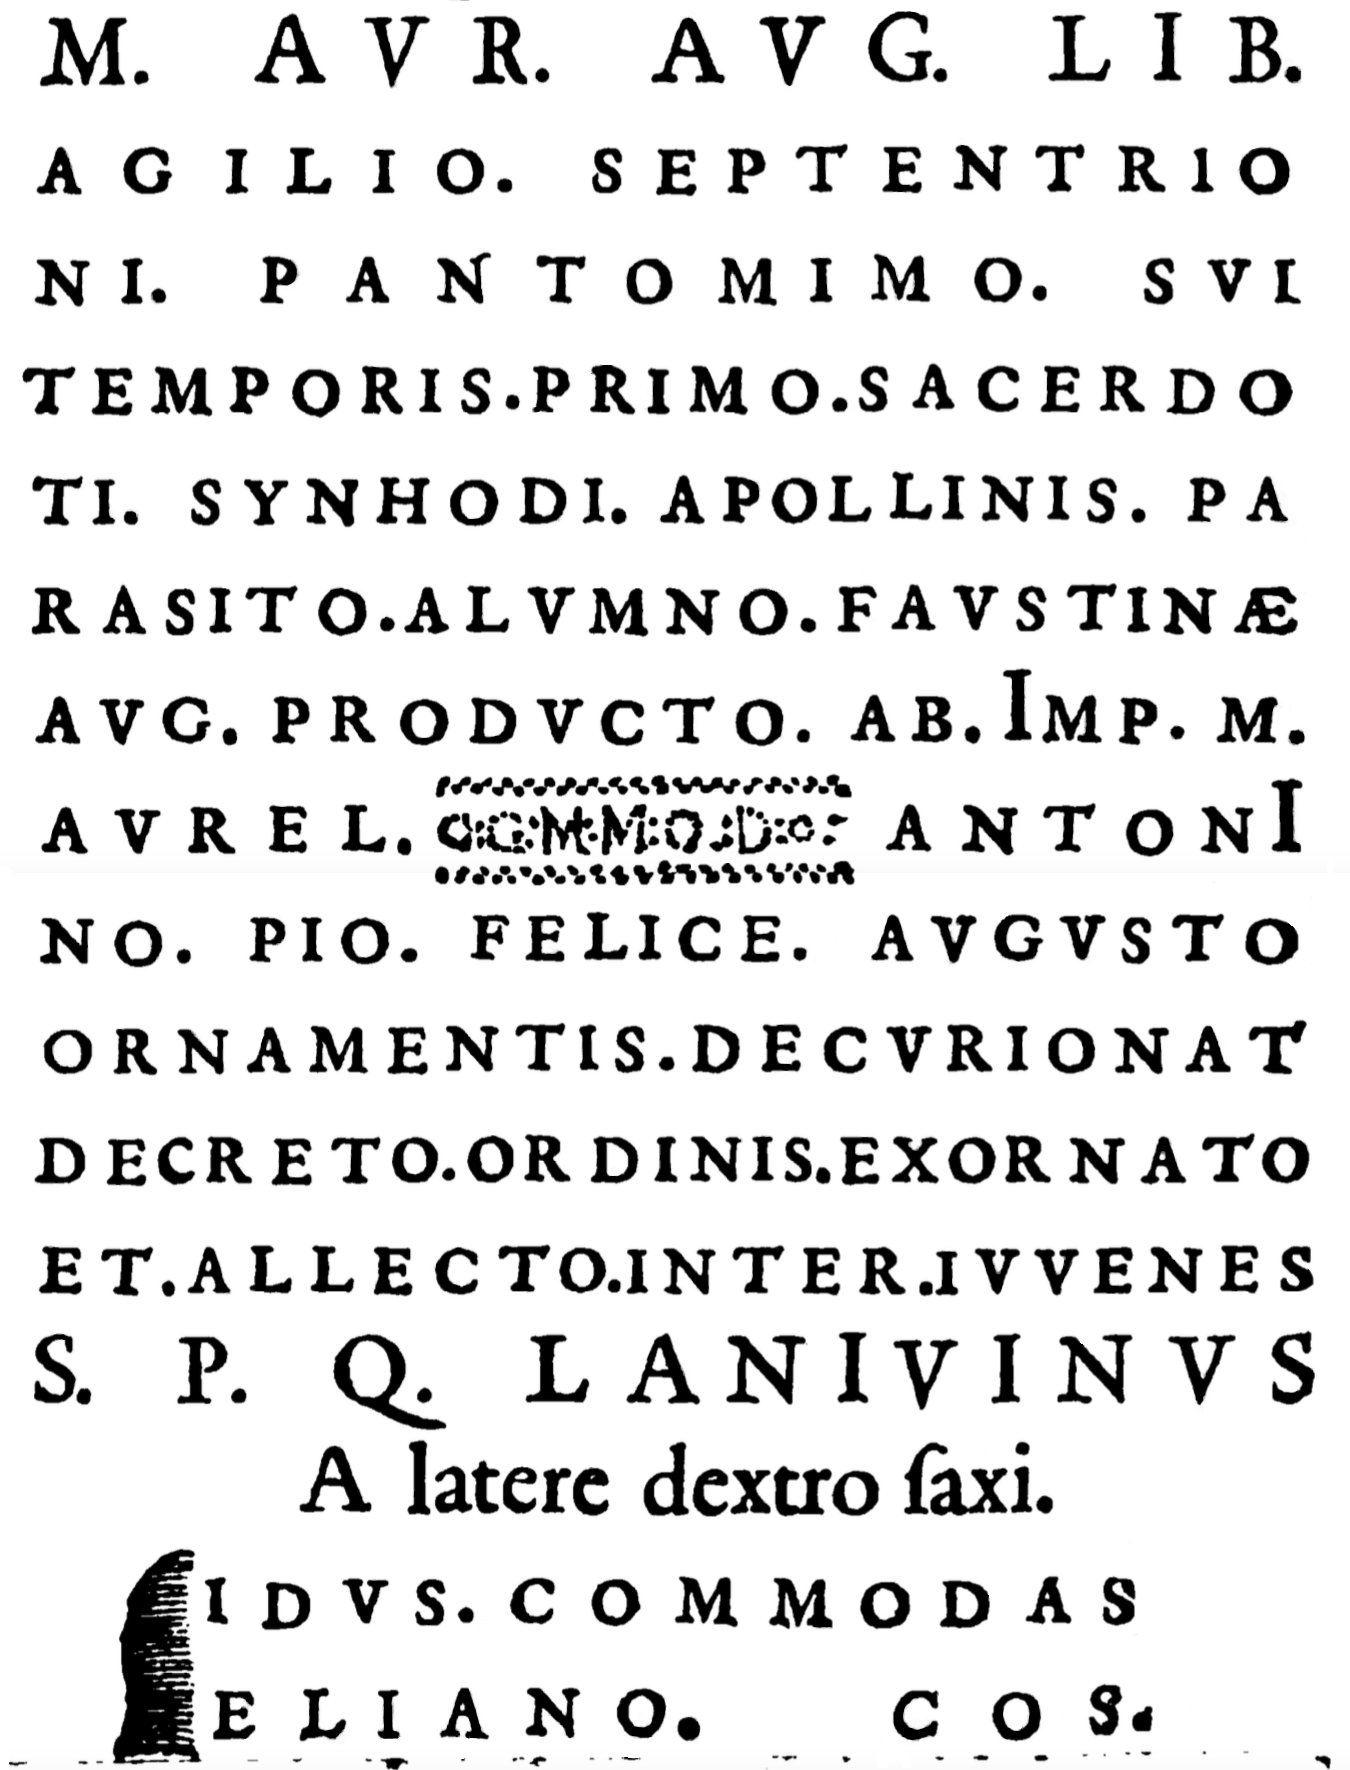
\includegraphics[scale=0.125]{011_lapis_lavinii}
  \caption{Lapis Lavinii}
  \label{fig:lapis_lavinii}
\end{figure}
\lnr{25}Martialis:
 \textit{Dum Ianus hiemes, Domitianus
autumnos}, et cetera.
\lnr{27}Sed Statius omnes
Kalendas vindicat Domitiano,
praeter Iulium, et Augustum,
– \textit{Nondum omnis honorem
Annus habet, cupiuntque decem tua
nomina menses.}
\lnr{32}Insania quoque
Commodiidem consecuta esset, si
longior vita monstro illi data fuisset.
% ō -> on (2x)
Augustum enim Commodum,
% ō -> om
Septembrem Herculeum, Octobrem
Invictum, Novembrem
Exuperatorium, Decembrem
Amazonium vocari edicit.
\lnr{39}Extat
quoque lapis Lavinii, in quo mentio
Iduum Commodarum.
% There is also a stone in Lavinus, which mentions "the ides of Commodus"
\lnr{41}Ubi et
nomen Commodi Senatusconsulto prius derasum, postea alia manu
incisum.
% "And where the name of Commodus was earlier erased by decree of the senate,
% a later hand inscribed it (again)."

% 12
% {PDF page nr}{source page nr}{line nr}
\plnr{95}{12}{3}Quaedam nationes etiam geminos menses cognomines habent.
\lnr{4}Annus Syrochaldaicus habet geminum Tisrin, item geminum Conum.
\lnr{5}Annus Hagarenus geminum Regiab, et geminum Giumadi.
\lnr{6}Annus Saxonicus geminum Giuli, et geminum Lida.
\lnr{6}Sed in
anno embolimaeo Lida est tergeminus.
\lnr{7}Et tunc annus ille dicebatur
Trilida.
\lnr{8}Item, diversarum nationum iidem menses communes.
\lnr{8}Nam
Panemus in anno Macedonico fuit, item Corinthiaco, et Thebano.
\lnr{10}Artemisius communis fuit Laconum, et Macedonum: Carneus Syracusanis,
et Cyrenensibus usitatus.
\lnr{11}Sed differbant situ anni et tempore:
ut suo loco disputabitur.
\lnr{12}Sic Martius primus erat Romanorum:
tertius Albanorum, Aricinorum, Formianorum: quartus Forensium,
Pelignorum, Sabinorum: quintus Faliscorum, Laurentum:
sextus Hernicorum: decimus Aequicolorum.
\lnr{15}Haec in genere
de mensibus.

\section{De Anno}

\lnr{17}Maximum \textgreek{[Greek]}
 dierum annus, sed qui multipliciter dictus
sit.
\lnr{18}Tot enim constitui possunt, quot sunt siderum errantium
periodi.
\lnr{19}Est enim annus circuitus eius periodi, cuius cognominis
ipse est.
\lnr{20}Ut annus Solaris est cognominis circuitus eius sideris,
qui quidem circuitus dupliciter sumitur.
% Started new sentence here. Original has comma. New sentence fits better
% with comming sentences.
\lnr{21}Aut ab Solstitio ad Solstitium,
% à -> ab
ab bruma ad brumam: et est minor anno Iuliano.
% à -> ab
\lnr{22}Aut ab puncto Zodiaci,
% à -> ab
ad idem punctum Zodiaci, qui est maior anno Iuliano.
% Changed point to comma, to get same sentence structure as previous one.
\lnr{23}Hoc est maior 365~\myfrac{1}{4} diei.
\lnr{24}Quo ad id punctum Zodiaci redit, unde profectum
erat.
\lnr{25}Eadem fere quantitas quae et Soli, attribuitur Veneri et Mercurio.
\lnr{26}Saturni periodus est dierum 10747.18'.59''.13'''.
\lnr{26}Hoc est annorum
Aegyptiorum 29. dierum 162.
\lnr{27}Iovis annus dierum 4330. horarum 17.14'.
\lnr{28}Id est annorum Aegyptiorum 11.315.
\lnr{28}Martis annus dierum
686. horarum 22.24'.
\lnr{29}Annorum Aegyptiorum 1.321 dierum.
\lnr{29}Lunae,
dierum 29.31'50''.8'''.
\lnr{30}Obtinuit tamen vulgo, ut duorum siderum,
Solis et Lunae, labentem coelo qui ducunt annum, ratio in temporibus
civilibus haberetur.
\lnr{32}Et Lunae quidem primum unus circuitus
pro anno habebatur, ut apud Aegyptios.
\lnr{33}Deinde tres, ut apud eosdem
Aegyptios et Arcades.
\lnr{34}Tandem duodecim periodi Lunares annum
civilem constituerunt dierum 354 cum triente, et paulo plus quam
duum trientum horariorum.
\lnr{36}Duodecim quoque segmenta Zodiaci
componunt annum Solarem tantum, quantum diximus.
\lnr{38}Sed ignoratio
motuum utriusque sideris alias atque alias anni formas veteribus
peperit:

% 13
% {PDF page nr}{source page nr}{line nr}
\plnr{96}{13}{1}quarum vetustissima est ea, quae annum quidem ad cursum
Lunae describebat:
\lnr{2}sed incertis neomeniis, quae non prodeunt ex observatione
motus Lunae, quales vulgus rusticorum observare solet, et
quae proprie civilem mensem constituere non possunt.
\lnr{4}Cum igitur
hoc modo incertae essent neomeniae, convenit primum, ut menses omnes
tricenis diebus explicarent, annumque dierum sexaginta et trecentum
constituerent.
\lnr{7}Quod genus longe desciscebat ab modo anni
% à -> ab
Lunaris.
\lnr{8}Haec diu seruata fuit apud Graecos anni forma.
\lnr{8}In Oriente
septuagesima secunda pars illius anni, hoc est quinque dies, accesserunt
anno Graeco: ut anni modus fuerit dierum trecentorum sexaginta quinque:
qua ratione ab anno solari se minimum discedere arbitrati sunt.
\lnr{12}Unde duo praecipua genera anni apud veteres suerunt neque Lunaria,
neque Solaria, sed ambigui inter utrumque generis.
\lnr{13}Prior forma in
Graecia resedit: altera in Oriente.
\lnr{14}Graeci vero non una via ad emendationem
suae aggressi sunt.
\lnr{15}Difficile erat menses plenos omnes ad
Lunae rationes exigere: et tamen in quibusdam actibus civilibus opus
habebant motu Lunae.
\lnr{17}Nam semper Olympias plenilunio, et \rnum{xv}
die mensis celebrabatur.
\lnr{18}Ut igitur annus Graecus aequabilis Olympiadem
deprehenderet in \rnum{xv} mensis, hoc difficile non erat.
\lnr{19}Ut autem
\rnum{xv} mensis in \rnum{xv}
 Lunae incidat in mensibus aequabilibus, hoc fieri non
potest, nisi post fingula quadriennia, adiectis unicuique anno singulis
biduis, quas \textgreek{[Greek]} vocabant.
\lnr{22}Haec Tetraeteris Elidensibus
vocata est Olympias, Delphis Pythias.
\lnr{23}Eiusque mensis primus duantaxat
erat Lunaris: reliquorum ratio claudicabat.
% written as: claudicābat. Probably a smudge. Other copies don't have the bar.
\lnr{24}Primus Cleostratus
eum annum in Lunarem modum reformare conatus est, excogitata
octaeteride dierum 2922, cuius menses alternis pleni et cavi: anni vero
singuli communes 354 dierum: embolimaei 384. communes quidem
quinque, embolimaeitres.
\lnr{28}Syzygiae autem novem et nonaginta.
\lnr{28}Octaeteridum
vitio deprehenso, Meton enneadecaeterida excogitavit dierum
solidorum 6940.
\lnr{30}Cui castigandae periodus Calippica successit dierum
27759, sine ullis scrupulis appendicibus, anno ab editione Metonica
centesimo tertio.
\lnr{32}Hanc excepit ultimus, tanquam secutor quidam,
Hipparchus, annis circiter centum octoginta octo ab epocha Calippica,
periodo publicata dierum 111035: quae minor est Calippicis rationibus
die uno, Metonicis autem quinque.
\lnr{35}Quare duae castigationes adhibitae
anno aequabili Graeco.
\lnr{36}Altera est coniugatio alterna vel interrupta
mensium plenorum et cavorum, ut cum ipsa Luna congruerent, quod
annus Graecus maior esset Lunari.
\lnr{38}Altera est embolismus mensium, ut
cum sole aequaretur, quod annus Lunaris minor est Solari.
\lnr{39}Sed alternatio
plenorum et cavorum mensium aliquando variat: idque fit aut
naturaliter, aut civiliter.
\lnr{41}Naturalis varietas committitur propter embolismum
aut mensis, aut diei.

% 14
% {PDF page nr}{source page nr}{line nr}
\plnr{97}{14}{1}Utroque enim modo duo menses pleni continuantur.
\lnr{2}Ut in anno Iudaico cum intercalatur mensis Adar, tunc
Schebat, et Adar embolimus ambo sunt pleni.
\lnr{3}In anno vero Arabico
cum accedit dies mensi ultimo, qui Dulhagiathi dicitur, tunc et ipse
Dulhagiathi, et antecedens Dulkaadathi ambo fiunt tricenum dierum.
\lnr{6}Sed in Samaritano saepe continuantur tricenarii menses, et in antiquo
Iudaico, ut ex Talmud et Iad Mosis cognoscimus: et menses Harpali,
Metonis, et Calippi non semper alternis continuati sunt.
\lnr{8}Sed saepe bini
pleni continuati, nunquam autem bini cavi.
\lnr{9}Quin etiam cum dies accedit
ultimo mensi Arabico, tres continui menses sunt pleni, Dulkaadathi,
Dulhagiathi, et Muharam sequentis anni.
\lnr{11}Isque annus ab Arabibus
dicitur \textarabic{[Arabic]} hoc est embolimaeus.
\lnr{12}Sic etiam anno Iudaico pleno
tres menses continui sunt pleni, Tisri, Marchesuvan, Casleu.
\lnr{13}Civilis
varietas accidit anno Iudaico tantum, accrescente mensi Marcheschuvan
die uno: et Marchesuvan ex cavo sit plenus.
\lnr{15}Rursus et in embolismo
mensium differentia situ, et tempore.
\lnr{16}Situ, si aut in medio, aut in calce
intercalatio fiat.
\lnr{17}Ut in anno Attico ultimus mensis intercalabatur, qui
dicebatur \textgreek{[Greek]}.
\lnr{18}In Iudaico sextus mensis intercalatur, et
dicitur Adar prior.
\lnr{19}In anno Hagereno mensis embolimus erat desultor,
qui omnes menses anni percurrebat in annis 228, quae sunt enneadecaeterides
duodecim.
\lnr{21}Qua intercalatione memoria proavorum nostrorum
utebantur Turcae Cilices, donec annum Hegirae simplicem
Muhamedicum usurpare coeperunt.
\lnr{23}At in anno prisco Romanorum
situs embolismi longe diversus ab aliis.
\lnr{24}Non enim is inter duos
menses interiiciebatur, ut alias solet: sed in mensem ipsum, tanquam
surculus in truncum infindebatur.
\lnr{26}Inter \rnum{xxiii} enim, aut \rnum{xxiiii},
aut inter \rnum{xxii}, et \rnum{xxiii} Februarii inserebatur.
neque vero sine caussa.
\lnr{28}Hoc enim semper observabant, ut mensis proximus Martio semper esset
dierum \rnum{xxviii}.
\lnr{29}Eratque Februarius ordinarius.
\lnr{29}At intervallum inter exitum
Ianuarii, et Kalendas Februarii ordinarii imputabatur Merkedonio.
\lnr{31}Et Kelendae Februarii ordinarii in anno embolimaeo nunc in Regifugium,
nunc in Terminalia, incurrebant.
\lnr{32}Neque enim semper inter
Terminalia, et Regifugium intercalabantur, ut vult Censorinus.
\lnr{34}
Quia hoc pacto Februarius ordinarius nunc viginti octo; nunc undetricenum
dierum fuisset.
\lnr{35}Quod tamen falsum ex Varrone convicitur.
% conuicitur: better visable in other copy
\lnr{36}Tempore differt intercalatio, quatenus Iudaei nunquam intercalant,
priusquam \textgreek{[Greek]}, qui sunt dies decem cum horis paulo
magis quam una et viginti, eo rationes Solis deduxerint, ut commode
mensis Lunaris conflari possit.
\lnr{39}Quod spatium numquam maius est
triennio, nunquam minus biennio: et in \rnum{xix}. annis semper septies fit.
\lnr{41}At in Calippico et Metonico anno aliquando citius, aliquando ferius
intercalabatur, quam ratiocinia \textgreek{[Greek]} postulare videntur.

% 15
% {PDF page nr}{source page nr}{line nr}
\plnr{98}{15}{2}Quandoquidem hoc unum cavent praecipue Athenienses,
 ne Hecatombaeonis
neomenia Solstitii priscam epocham antevertat: cum in
% neomenia: better visable in other copy
anno Iudaico ut plurimum neomenia Tisri aequinoctium autumnale,
neomenia vero Nisan aequinoctium veris antiquum, si ratio Iuliani
anni habeatur, antevertat.
\lnr{6}Anni Lunaris non unum genus est: sed
summa divisio in duo fastigia discedit: in annos periodicos, et simplices.
\lnr{8}Anni periodici dicuntur, qui certo annorum orbe, interventu
embolismorum, recurrunt.
\lnr{9}Huius intervalli modum veteres certo
definire non potuerunt.
\lnr{10}Quippe Cleostratus dierum 2922, Harpalus
2924, Eudoxus plusquam 2922, minus quam 2924: Meton aliter:
et ab omnibus diverse Calippus, et denique ab eo discedens Hipparchus.
\lnr{13}Cuius sententia, sed caelestibus rationibus leviter castigata,
 enneadecaeterida
% έννεακαιδεκα-ετηρίδα: Meton cycle, or "Great Year". Nine-and-ten anniversary
% ετηρίδα: anniversary
% Search "Enneadecaeteris" on Wikipedia to give the "Metonic cycle" page.
Lunarem minorem Iuliana statuit, hora una cum scrup. [?] paulo
% What is "scrup." short for? scrupula? See also p.17, 18
plus quam viginti septem.
\lnr{15}Simplices anni et ipsi quidem sine remedio
intercalationis in pristinam epocham recurrunt, sed longo intervallo,
annorum scilicet Iulianorum 228, qui sunt anni simplices Arabici 235,
scrupuli diurni quinquaginta.
\lnr{18}Sunt et in annis Lunaribus cavi, superflui,
aequabiles.
\lnr{19}Annus cavus is est, cui competit \textgreek{[Greek]}.
\lnr{20}Ideo ab nobis \textgreek{[Greek]} vocabitur.
% à -> ab
\lnr{20}Ex eo enim eximitur dies
vel propter civile institutum, cuiusmodi est annus Iudaicus,
quem defectivum
Computatores Iudaeorum vocant.
\lnr{22}(In eo quippe Casleu, qui natura est plenus, instituto fit cavus.)
% Casleu: Hebrew כִּסְלֵו, Kislev, the third month of the civil year
% (9th of ecclesiastical year) in the Hebrew calendar.
\lnr{23}Vel naturali de caussa: ut anno
decimonono Cycli Paschalis Dionysius diem unum eximit, quem
vocavit Saltum Lunae: Graeci vero Computatores
 \textgreek{[Greek]}.
\lnr{26}Quamquam inepte annum ultimum enneadecaeteridis constituit dierum
duntaxat 353, cum eiusmodi annus natura nullus fit.
\lnr{27}Superfluus
annus vocetur ab nobis \textgreek{[Greek]}.
% à -> ab
\lnr{28}Accedit enim illi \textgreek{[Greek]}
tam ex caussa civili, ut in anno Iudaico Marcheschuvan naturaliter
cavus, civiliter fit plenus: quam e caussa naturali: ut undecim anni
in Triacontaeteride Arabica augentur singulis diebus ex ratiociniis
Lunae collectis.
\lnr{32}Annus aequabilis vocetur \textgreek{[Greek]}.
\lnr{32}Iudaeis computatoribus
dicitur annus ordinarius.
\lnr{33}Is est, cui nihil accedit, nihil decedit.
\lnr{34}Huc usque ad annum Lunarem deduxit nos aequabilis minoris
disputatio.
\lnr{35}Nunc de altero aequabili maiore disputandum, quo Aegyptii,
Persae, et Armenii, Mexicani, et Perusiani usi.
\lnr{36}Hic antiquitus
Orientis nationibus unus idemque fuit: praeter quam si quando
 \textgreek{ἐπαγόμεναι [Greek]}
% Epagomenal days are days within a solar calendar that are outside
% any regular month.
quinque in alium locum traductae, diversum anni caput constituebant.
\lnr{39}Qua \textgreek{ἐπαγομένον [?]} tralatione utebantur ii,
 qui post annos 120
aequabiles mensem solidum intercalabant, ut Persae: qui quidem
 \textgreek{ἐπαγόμενας[Greek]}
suas in aequinoctium vernum semper reiiciebant.
\lnr{41}Terminum autem vocabant \textsc{nevruz}.
% https://en.wikipedia.org/wiki/Nowruz
% Persian: نوروز‎‎ litterary "New Day"

% 16
% {PDF page nr}{source page nr}{line nr}
\plnr{99}{16}{1}Et habebant mensem desultorem
% mensem desultorem = leap month?
\textgreek{ἐμβὀλιμον [?]}, omnes menses anni pervagantem, donec in primum
% Embolismic month: 13th intercalary month inserted in the year.
mensem recurreret.
\lnr{3}Qui orbis non redibat, nisi anno aequabili 1461
vertente, qui sunt anni Iuliani perfecti 1460.
\lnr{4}Hic est magnus annus,
cuius menses sunt annorum aequabilium tricenum, quot dierum simplex
mensis.
\lnr{6}\textgreek{ἐπαγόμεναι [?]} autem sunt quinquies quatuor annorum, ut
illae simplices quinque dierum.
\lnr{7}Quod autem illa anni forma retenta
fit, in caussa fuit non tam ignoratio annis solaris,
 quam facilis, et tractabilis,
ac vere popularis eius usus.
\lnr{9}Alioqui nulla fere natio fuit, quae
quadrantem anni Solaris ignorarit: sed modum illius dispensandi
nesciebant.
\lnr{11}Praeterea ab mensibus superfluis, qui sunt maiores tricenis
% à -> ab
diebus, refugiebant, quos necesse est retincri,
 quadrante illo retento.
\lnr{13}Aegyptii singulis quadrienniis exactis diem intercalabant
 in ortu Caniculae,
et quadriennium illud exactum \textgreek{[Greek]}, \textgreek{[Greek]},
\textgreek{[Greek]}, vocabant.
\lnr{15}Attici diem quarto quoque anno exacto intercalabant
inter septimum et octavum diem Ianuarii.
\lnr{16}Elidenses inter
octavum, et nonum Iulii.
\lnr{17}Syromacedones, Chaldaei, et Iudaei inter
septimum et octavum Octobris.
\lnr{18}Eamque diei intercalationem ab Seleucidarum
% à -> ab
temporibus usque ad imperium Constantini et infra retinuerunt
Iudaei: quam utique simul cum anni Calippici forma ab victoribus
% à -> ab
Syromacedonibus acceperant.
\lnr{21}Romani Atticos secuti brumae
sidere confecto intercalabant; quae ipsis Olympiadum mysteria vocabantur.
\lnr{23}Nam et Attici et reliqui omnes Graeci annum Solarem in
quatuor quadrantes dividebant, quae \textgreek{κέντρα [?]}
 vocabant, singulis dies 91.
hor. 7~\myfrac{1}{2} attribuentes.
\lnr{25}Quod ab temporibus Seleucidarum, ad hanc usque
% à -> ab
diem, Iudaei constanter observant.
\lnr{26}Itaque \rnum{viii} Iulii erant \textgreek{[Greek]},
\rnum{vii} Octobris \textgreek{[Greek]}:
 \rnum{vii} Ianuarii \textgreek{[Greek]}, \rnum{viii}
Aprilis \textgreek{[Greek]}.
\lnr{28}Quare cum legis \textgreek{[Greek]}, et \textgreek{[Greek]},
nullas alias intellige, praeter has.
\lnr{29}Quod et \textgreek{[Greek]} quoque intelligendum.
\lnr{30}Haec \textgreek{κέντρα [?]} Iudaei Tekuphoth vocant.
\lnr{30}Germani, Celtae,
Saxones inter \rnum{xxv} et \rnum{xxvi} Decembris intercalabant:
 quam noctem
vocabant \textsc{mudranecht}.
\lnr{32}Tartari hodie inter ultimam Ianuarii,
et Kalendas Februarii, quas Kalendas patrio sermone Festum Alborum
% comma for period
vocant, quia albis vestibus eam diem colunt.
% comma for period
\lnr{34}Denique quanuis
Lunari anno, aut alio longe diverso ab Solari uterentur, tamen tacita
% à -> ab
quadam observatione post dies 1460 unum diem intercalandum esse
sentiebant.
\lnr{37}Neque enim aliter Habraei quatuor Tekuphas suas tueri
potuissent, nisi quadrante post quartum quemque annum rationibus accedente.
\lnr{39}Et sane unaquaeque Tekupha est dierum 91, horarum 7~\myfrac{1}{2}.
% Period inserted
\lnr{39}Unde
quatuor tantae Tekuphae fiunt dies 365~\myfrac{1}{4}.
\lnr{40}Displicuit tamen haec quadrantis
observatio Graecis Astronomis, propter causam admodum futilem
et puerilem, qua Solis quantitatem ad Lunae ratiocinia exigebant,
et cum utriusque sideris exactum modum adhuc non tenerent,
ex Lunae comparatione Solares rationes eliciebant.

% 17
% {PDF page nr}{source page nr}{line nr}
\plnr{100}{17}{3}Itaque tantam
censuerunt Solis quantitatem, quantam summam dies periodi in annos
periodi distributae relinquebant.
\lnr{5}Metonis periodus est dierum
6940.
\lnr{6}Divisa per 19 annos relinquit quantitatem anni Solaris Metonici
dierum 365. scrup. diurnorum 15~\myfrac{5}{19} Calippi periodus dierum
% Again "scrup.". See also p.15, 18
27759 per 76 annos divisa relinquit modum anni Calippici Solaris
dierum 365~\myfrac{1}{4}.
\lnr{9}Qualis est annus noster Iulianus.
\lnr{9}Periodus Hipparchi
est dierum 111035, annorum 304.
\lnr{10}Sed neglectis illis 4,
trecentesima pars diei detrahitur de quantitate anni Calippici Solaris,
ut fiat annus Solaris Hipparcheus
 dierum 365. hor. 5. 55.' 15.'' \myfrac{15}{19}
\lnr{13}Detractis ex quadrante hor. 0. 4.' 44.'' \myfrac{4}{19}
 quae etiam fuit sententia
Ptolemaei.
\lnr{14}Itaque ex sententia Hipparchi et Ptolemaei annus
Tropicus, est annus Iulianus, vel Calippicus nonadecima parte
differentiae enneadecaeteridis Lunaris et Iulianae diminutus: qui
est verus annus Rabbi Ada: de quo alibi.
\lnr{17}Philolai Pythagorei magnus
annus dierum 21505~\myfrac{1}{2} per 59 annos divisus constituit modum
Solarem dierum 365.
\lnr{19}Oenopidae annus magnus dierum 21557
itidem per 59 annos divisus dat modum anni Solaris dierum 365 cum
parte dierum duum et viginti undesexagesima.
\lnr{21}Harpali octaeteride per
8 annos divisa remanet modus anni Solaris dierum 365~\myfrac{1}{2}.
\lnr{22}Annus magnus
Democriti dierum 29950~\myfrac{1}{2} per 82 annos divisus relinquit annum
Solarem dierum 365, cum quadrante et centesima sexagesimaquatra
parte unius diei.
\lnr{25}Denique nullus veterum non putavit rationes
Solis ad Lunam exigendas esse.
\lnr{26}Et quotiescunque ex certa collectione
dierum utriusque sideris rationes congruerent, dies illi per tot
annos divisi, quot ex illa summa dierum constitui poterant, visi sunt
illis certam anni Solaris quantitatem definire posse.
\lnr{29}Sapientiores vero,
quanuis incomprehensibilem illam existimarent, tamen pro vero quod
proximum putabant amplexi sunt, dies trecentos sexaginta quinque
cum quadrante, qui est modus anni Iuliani.
\lnr{32}Cui singulis quadrienniis
exactis unus dies accrescit.
\lnr{33}Sed hic annus comparatione Aegyptiaci
est Solaris: comparatione autem Tropici est aequabilis.
\lnr{34}Maior
enim est vera anni ratione scrup. horariis 11.' 6.'' 40.'' secundum
% Again "scrup.". See also p.15, 18
Gelalaeam formam, aut 10.' 48.'' fere, ut Alfonsini docent.
\lnr{36}Neque
Prutenicae tabulae multum abludunt, quae constituunt motum
aequalem Solis ab aequinoctio dierum 365. Hor. 5. 49.' 15.'' 46.'''
\lnr{39}Itaque hinc nasci possunt aliquot genera anni Solaris.
\lnr{39}Aequabilis,
ut Iulianus.
\lnr{40}Tropicus, ut Persarum Gelalaeus.
\lnr{40}Rursus Tropicus
aut aequabilis, aut caelestis.
\lnr{41}Aequabilis
Tropicus, cuius quantitas
Tropica est, partes autem, hoc est menses, aequales et civiles: ut is,
quem modo dixi, Galelaeus.

% 18
% {PDF page nr}{source page nr}{line nr}
\plnr{101}{18}{2}Descriptus est enim mensibus aequalibus,
omnibus tricenum dierum, cum epagomenis appendicibus, quae
in communi anno sunt quinque, in embolimaeo sex.
\lnr{4}Caelestis Tropicus,
cuius partes in naturalia Zodiaci segmenta tributae sunt.
\lnr{5}Rursus
et annus Solis aequabilis in civilem et caelestem dividi potest.
\lnr{6}Civilis,
ut Iulianus Romanorum, Syrograecorum, Graecorum Elkupti.
\lnr{7}Caelestis,
ut Dionysianus Prolemaei Philadelphi.
\lnr{8}Nam et is quoque quadrantem
Canicularem quadriennio exacto accipiebat.
\lnr{9}Finis vero
omnis periodi is est, ut caput recurrat et revoluatur in idem principium,
quam \textgreek{[Greek]} Graeci vocant: quae quidem pessum iverit tandem,
non seruata veri anni Tropici mensura.
\lnr{12}Et quia annus Iulianus
suam tueri non potuit, manifestum est Kalendas Ianuarias ab \rnum{viii}
parte Capricorni, in qua statuerat eas Caesar, in vicesimam primam
fere traductas esse hodie.
\lnr{15}Sed nihilo commodius epocha in enneadecaeteride
seruari potest.
\lnr{16}Nam enneadecaeteris Tropica est velocior
Lunari horis plusquam duabus.
\lnr{17}Contra enneadecaeteris Iuliana
maior Lunari hora una, et scrup. plusquam 26.
% Again "scrup.". Scrupulus? See also p.15, 17.
\lnr{18}Cum vero peccatur
utraque ratione, Tropica et Iuliana, Luna, cuius rationes mediae sunt
inter illas duas, fines epochae suae tueri non potest: ut in cyclo Dionysii
Paschali accidit, cuius neque rationes ad enneadecaeterida Lunarem
collectae sunt, neque epocha ad Solis motum castigata: sed eius
forma potius tota mere Calippica est.
\lnr{23}Ita ut eius statum post trecentos
4 annos variare necesse sit.
% 4. -> 4
\lnr{24}Quare ut epochat suas servarent illi veteres,
immanes periodos excogitaverunt, quales illae Calippi, Philolai, Democriti,
Oenopidae.
\lnr{26}Sunt etiam periodi, quae omnem modum excedebant.
\lnr{27}Et cum in omnibus illis orbibus annorum praecipuam
utriusque sideris rationem haberent, tamen nescio quae confidens eos
incessebat opinio, non solum utriusque sideris, sed etiam omnium
\textgreek{[Greek]} illo circuitu fieri.
\lnr{30}Sic Harpalus et Eudoxus putarunt
in sua Octaeteride omnes \textgreek{[Greek]}
 et \textgreek{[Greek]} in orbem redire.
\lnr{32}Idem etiam censet fieri Aratus in Metonica enneadecaeteride, Eudoxum
suum sectus, qui in fabrica Sphaerae suae eam planetarum et inerrantium
harmoniam in eorum orbibus ostendit esse, ut sequente
restitutione utriusque sideris, necessario et omnium inerrantium reditum
contingere concluderet.
\lnr{36}Propterea tot Sphaeras \textgreek{[Greek]} commentus
est, quot narat Aristoteles libro \rnum{xi} \textgreek{[Greek]} quem
consulas licet.
\lnr{38}Quin etiam Calippus alios orbes praeter Eudoxum
addidit, ea ratione, ut \textgreek{[Greek]} adstrueret,
 \textgreek{[Greek]},
ut Aristoteles de ea re scribens pronunciavit.
\lnr{41}Itaque \textgreek{[Greek]} nomine intelligendum ortus,
 et occasus \textgreek{[Greek]},
non autem \textgreek{[Greek]}, hoc est significationes
eorum: quas in orbem redire cum Luna et Sole in enneadecaeteride
Meto quidem, Calippus, et Hipparchus putarunt, et aliis
persuaserunt, donec deprehenso vero anni Tropici modulo vitium
harum periodorum castigatum est.

% 19
% {PDF page nr}{source page nr}{line nr}
\plnr{102}{19}{5}Cicero quoque apud Macrobium,
sexto de republica, annum illum immanem, quem ex tot millibus
annorum simplicium componit, non aliter in orbem rediturum
cum omnibus errantibus et inerrantibus censet, quam si eadem defectio
Solis in eodem loco, eodem tempore fiat: quanuis defectiones
cyclo enneadecaeterico recurrant non raro.
\lnr{10}Et tamen ea eclipsi putat
non tantum Solis et Lunae, sed etiam quinque errantium ad eandem
inter se comparationem, confectis omnium spatiis, reditum fieri, quo
eadem caeli positio, siderumque, quae ab initio maxime fuit, rursus existit.
\lnr{14}Quare eclipses ad eam rem notabant veteres, ut etiam
 \textgreek{[Greek]}
\textgreek{[Greek]} excogitarint.
\lnr{15}\textgreek{[Greek]} vocabant.
\lnr{15}Eorum vetustissimus fuit
dierum 6585~\myfrac{1}{3}, qui sunt anni Arabici 18, syzygiae 7.
\lnr{16}In genere vero
sunt syzygiae 223.
\lnr{17}Quamobrem in secundo libro Plinii perparem legitur
sive culpa ipsius Plinii, sive librarii, defectus luminum ducentis
viginti duobus mensibus redire.
\lnr{19}Hipparchus alium \textgreek{[Greek]} longe
maiorem excogitavit dierum 126007, syzygiarum 4267, annorum
Arabicorum 355 cum syzygiis 7: annorum Iulianorum 344 cum
diebus 361.
\lnr{22}Quae sunt tolerabiles periodi.
\lnr{22}Nam ab caussis naturalibus,
% à -> ab
nempe ab defectionibus luminum proficiscuntur.
% à -> ab
\lnr{23}Quemadmodum
etiam enneadecaeteris Lunaris, et Cyclus Solis: quorum illa Lunam
Soli restituit, hic Solem Septimanae, et praeterea periodus Mexicanorum
constans annis \rnum{lii}, quae restituit
 \textgreek{[Greek]}, quae ist ipsis
vicem nostrae Hebdomadis.
\lnr{27}Neque alia fuit periodus magna Persarum
veterum, quam Salchodai vocabant.
\lnr{28}Sunt et aliae, sed civiles, et Indictio;
Aliae inanibus coniecturis insistunt, ut Dodecaeteris Chaldaica
Genethliacorum, item Heracliti, Lini, Orphei, Dionis, et Magorum:
quorum periodus ad modum octavae sphaerae composita est annorum
360000 ab conditu Mundi, ut ipsi putant.
% à -> ab
\lnr{32}Quorum annorum hic est
centies octagies quater millesimus, sexcentesimus nonagesimus quartus.
\lnr{34}Sed longe illa Sinarum prodigiosior, iuxta quam hic annus Christi
1594 est ab conditu rerum octigenties octagies quater millesimus,
% à -> ab
septingentesimus septuagesimus tertius.
\lnr{36}Bonziorum vero Iaponensium
periodus annorum 470 desivit cum anno Christi 1561. et 1562
coepit sequens.
\lnr{38}Eiusque hic est vicesimus currens.
\lnr{38}Ea vertente scelera
extirpatum iri: reliquum tempus omnia pacata fore credunt.
\lnr{39}Taceo
diversas Christianorum, Iudaeorum, Samaritanorum de conditu rerum
opiniones: item Romanorum lustrum quinque annorum, saeculum
centum et decem.

% 20
% {PDF page nr}{source page nr}{line nr}
\plnr{103}{20}{1}Sunt et periodi Computatorum: ut Iudaea
annorum 6916, quae constat cyclis Lunaribus 364, Solaribus 247, periodis
magnis Dionysianis 13.
\lnr{3}Habetque tot cyclorum septimanas,
quot dierum septimanae sunt in anno Solari: tot periodos Dionysianas,
quot menses annus embolimaeus: tot cyclos Solares, quot cyclos
Lunares magnus cyclus Iudaicus.
\lnr{6}Itaque elegantissima est, et artificiosissima.
\lnr{7}Eiusque hic agitur annus 5354, anno Christi vulgari 1594.
\lnr{8}Et inibit 1595 annus eiusdem proximo autumno, unde omnes epilogismi
neomeniarum Iudaicarum.
\lnr{9}Periodus Dionysiana et ipsa ad
annalem computum pertinet, annis constans 532, ducto in sese utroque
cyclo.
\lnr{11}Verae quidem periodi magnae caput incurrit in annum
primum utriusque cycli, pertinetque ad methodum Lunae et Solis.
\lnr{12}Et
locum habet dumtaxat in anno Iuliano, hoc est in eo, cui praeter 365
dies quadrans attibuitur.
\lnr{14}Itaque eius initium est ab Kal. Ianuariis in
anno Romano: in anno Constantinopolitano ab Kal. Septembris. in
Antiocheno ab Kal. Octobris. in Alexandrino et Samaritano ab a. d.
\rnum{iiii}. Kal. Septemb.
% à Kal. -> ab Kal. (3x)
\lnr{17}Periodus vero Dionysii pertinet ad methodum
neomeniae Paschalis, initio sumto ab anno primo natalis Christi, ut
ipse quidem putabat: item ab anno decimo cycli Solis Iuliani, et ab
ea neomenia, cuius quartadecima dies proxime post
 \rnum{xxi}, aut in \rnum{xxii}
Martii conficeretur.
\lnr{21}Hactenus ab minimis initiis ad summa temporum
% à -> ab
incrementa, quam \textgreek{[Greek]} Graeci vocant, Chronologum
perduximus, et eum in conspectu totius antiquitatis collocavimus.
\lnr{24}Superest nunc, ut quae carptim et obiter perstrinximus, ea uberius
suis locis expicentur.
\lnr{25}Resumamus igitur eos annos, ex quibus tanquam
elementis, ad tot tamque diversa genera annorum progressus
factus est.
\lnr{27}Ex anno Graeco, qui est aequabilis minor, omnes anni, Lunaris
formas propagatas esse vidimus: ut ex Aegyptiaco, qui est aequabilis
maior, omnes Solares.
\lnr{29}Non igitur confuse, et per saturam haec
tractanda, sed suo quaeque et loco et ordine.
\lnr{30}Quatuor igitur libris
quatuor genera anni summa explicare decrevimus.
\lnr{31}Primus erit de
anno aequabili minore.
\lnr{32}Eo enim omnis Graecia usa tam diversis generibus,
quam multae fuerunt eius terrae nationes, et \textgreek{[Greek]}.
\lnr{33}Itaque
ea erit reliqua pars huius libri.
\lnr{34}Secundum locum sibi vindicat annus
Lunaris, quia ex illo priore derivatus.
\lnr{35}Tertius liber complectetur anni
aequabilis maioris formas, \textgreek{[Greek]}, et differentias.
\lnr{36}Quartus illius anni
traduces et propagines persequetur, diversa nempe anni Solaris genera,
et mutationes.
\lnr{38}Haec est pars prior, quam initio huius diatribae.
\lnr{39}Chronologo promisimus, de annorum et temporum Civilium generibus.
\lnr{40}Altera pars est de charactere, qui necessarius est notandis temporum
intervallis, quae sequentibus libris tractabimus, item diversis
computis nationum annalibus, de quibus librum singularem ad calcem
operis adiiciemus, non tanquam appendicem, sed partem unam
operis nostri.

% 21
% {PDF page nr}{source page nr}{line nr}
\plnr{104}{21}{3}Quis igitur sit usus characteris temporum, docet nos
Dionysius ex Ephoro, qui cum annum excidii Troiae ex Olympiadum
epocha notare non posset, cum is casus aliquot seculis antiquior
sit prima Olympiade, dixit id accidisse eo anno Attico, quo viginti
\textgreek{[Greek]} annum explebant.
\lnr{7}Statim peritis anni Attici subolebat,
quo anno id accidere potuerit.
\lnr{8}Sciebant enim quoties in quanto
intervallo annorum id fieri posset.
\lnr{9}Exemplo Ephori aut Dionysii
erit nobis character excogitandus, quo animus anceps in trivio constitutus
quaesitum ad fontem manu deducatur.
\lnr{11}Erit igitur primum
totius instituti nostri fundamentum annus Iulianus, quem fingimus
ante multa millia annorum fuisse.
\lnr{13}Characteres vero illi duos dabimus,
cyclum Lunae Dionysianum, cuius hic est annus \rnum{xviii}.
\lnr{14}Et cyclum
Solis Iulianum, cuius hodie annus \rnum{vii} currit.
\lnr{15}Tertium etiam,
ubi ratio temporum patietur, Indictiones non aspernabimur.
\lnr{16}Nam
qui his characteribus semel uti institerint, illi,
 quae sit constantia, et fides
illius methodi pulcherrimae in ratione temporum, experientur.
\lnr{18}Si
quis hoc anno Christi 1594 incertus, quot annos natus sit, tamen et
maiorem se quadraginta novem annorum, et minorem quinquaginta
sex sciat, is imitatur imperitiam Chronologorum Graecorum, qui
circiter illius, et illius regis tempora illud,
 et illud accidisse dicunt, annum
vero certum non difiniunt.
\lnr{23}Sed cum idem adiicit natum se Nonis
Augusti, feria quinta, is addit characterem certum et indubitatum,
quales sunt viginti \textgreek{[Greek]} Ephori.
\lnr{25}Nam feria quinta non
potuit incurrere in Nonas Augusti, nisi cum litera Dominicalis est C.
Ante 49 autem annos id accidit anno Domini 1540, cyclo Solis nono.
\lnr{28}Itaque hoc characterismo constantissime affirmanus eo anno hominem
natum, et proximis Nonis Augusti Iulianis illi quinquagesimum
quintum natelem initurum.
\lnr{30}Idem usus cycli Lunaris, adhibita
castigatione, ut ab prima Olympiade, ad annum Domini 1400, tot
% à -> ab
dies neomeniis adhibeas, quoties 304 annos reperies.
\lnr{32}Exemplum.
% Period after Exemplum: New sentence or different punctuation mark?
\lnr{33}Hic est annus ab prima Olympiade 2370.
% à -> ab
\lnr{33}In quibus annis septies reperitur
numerus 304.
\lnr{34}Septem igitur dies neomeniis hodiernis adiiciendi.
\lnr{35}Verbi gratia.
% Periods after numbers that do not indicate the end of a sentence
\lnr{35}Anno primo cycli epactae sunt \rnum{xi}. novilunium
Martii \rnum{xviii}. additis
 \rnum{vii}. diebus, novilunium, vel potius coniunctio
luminarium erat in \rnum{xxv}.
\lnr{37}Martii anno quarto ante primam Olympiadem,
aut quintodecimo post eandem primam Olympiadem, et deinceps
ad 304 annos.
\lnr{39}Sed ab hoc saeculo nostro post 150 annos minuendae
erunt neominiae totidem diebus, quoties 304 anni reperientur
post annum Christi 1700. et fortasse citius.
\lnr{41}Sed quia nullam epocham
veterem certiorem Olympiadum capite habemus: illud autem
cum vetustate comparatum novitium esse videtur: inutiles erunt characteres
cyclorum et Indictionis, nisi ab quadam remotissima epocha
% à -> ab
initium temporum instituamus.

% 22
% {PDF page nr}{source page nr}{line nr}
\plnr{105}{22}{4}Excogitemus igitur periodum,
quae et utrunque cyclum, et Indictionem contineat: quod fiet, si periodum
Dionysii Exigui quindecies multiplicemus: qui fient anni
7980.
\lnr{7}Ita periodus illa incipiet ab anno primo tum utriusque cycli,
tum Indictionis: et proinde eiusdem ultimus annus definit in ultimis
utriusque cycli, et Indictionis.
\lnr{9}Sed annus Christi, ut vulgo putamus,
3267 desinet in ultimum utriusque cycli, et Indictionis.
\lnr{10}Ergo deductis
3267 de 7980 annis, relinquetur epocha anni ante vulgarem
Christi, nempe 4713.
\lnr{12}Ita ut 4714 sit primus annus Christi vulgaris cyclo
Solis \rnum{x}, Lunae 2, Indictionis 4, ab Kal. Ianuarii: quamuis et Indictio
% à -> ab
autumno proxime antecedenti, Cyclus autem Lunae Martio sequenti
caeperit.
\lnr{15}Quare annus iste, qui ex errore vulgi putatur 1594, est 6307.
periodi huius, quam Iulianam vocamus, quod ad Iulianam anni formam
accommodata sit.
\lnr{17}Ideo 6307 divisis per 28, per 19, per 15 habebimus
huius anni 6307 periodi Iulianae, vel vulgaris Christi 1594, cyclum
Solis septimum ab Kal. Ianuarii:
\lnr{19}Lunae decimumoctavum ab
% à -> ab (2x)
Martio sequente:
\lnr{20}Indictionis septimum Caesarianae quidem ab ante d.
\rnum{viii} Kal. Octobris antecedentis anni 6306:
\lnr{21}Pontificiae vero ab Kalendis
% à -> ab
Ianuarii anni propositi 6307.
\lnr{22}Non praedicabo laudes huiusce periodi:
Chronologi et astrologi, qui omnia \textgreek{[Greek]} disputare volunt,
non poterunt eam satis laudare.
\lnr{24}Qui igitur eclipses ex Tabulis
% Tabulis: clearer in other copy.
Prutenicis putare volent, ex anno periodi Iulianae auferant 2408.
\lnr{25}Et
cum residuo toto excerperant tempora epochae diluvii.
\lnr{26}Exemplum: Eclipsis
Lunaris accidit in Septembri anno Olympiadico 446, qui est annus
periodi Iulianae 4383.
\lnr{28}Deductis 2408, remanent 1975.
\lnr{28}Excerpo
primum 1900 ex epocha Diluvii: deinde 75, ex filo annorum expansorum.
\lnr{30}Postremo menses usque ad Septembrem.
\lnr{30}Et reliqua ut ex methodo
Prutenica.
\lnr{31}Qui omne dubium ex temporum ratione tollere
volet, uti debet hac periodo, sine qua nihil unquam certi in natione
temporum adferre poterit.
% === End of the part entered as litteral transcript.

\section{De Anno Aequabili Minore Graecorum}
\lnr{34}Cum quidam veterum, ut Macrobius et Solinus, annum Graecorum
merum Lunarem fuisse prodiderint:
\lnr{35}neque solum in ea
haeresi fuerit vir eruditissimus Theodorus Gaza, sed et vetustissimum
scriptorem Herodotum opinionis suae testem adhibeat:
\lnr{37}equidem non
temere ab eius auctoritate discedendum esse censuissem, nisi hominem
clarissimum, atque utriusque linguae vindicem, in re manifesta
pueriliter erasse deprehendissem.

% 23
% {PDF page nr}{source page nr}{line nr}
\plnr{106}{23}{3}Is igitur ut probet menses Graecorum
Lunares, et alternis plenos et cavos fuisse, haec verba ex Herodoto
producit: \textgreek{[Greek]}.
\lnr{5}\textgreek{[Greek]}
\textgreek{[Greek]}
\textgreek{[Greek]}, \textgreek{[Greek]}.
\lnr{7}Videamus, an vera sit summi
viri sententia: et dies vicesies quinquies mille ac ducentos per septuaginta
annos partiamur.
\lnr{9}Prodit modus unius anni, dies trecenti sexaginta.
\lnr{10}Perperam igitur Lunarem annum definit, cuius menses omnes
fuerunt solidi.
\lnr{11}Duodecim enim menses omnes \textgreek{[Greek]}
annum habuisse, prodit Herodotus, non, ut ipse vult, alternis plenos
et cavos.
\lnr{13}Sed cum ea fuerit Gazae sententia, mirum, non contentum
fuisse hominem, unum Herodoti testimonium contra se produxisse,
nisi et Aristotelis altero ex libris \textgreek{[Greek]}
 loco magnam iniuriam
existimationi suae fecisset.
\lnr{16}Scribit enim Aristoteles eo, quem ipse
Gaza adducit, loco, \textgreek{[Greek]}, \textgreek{[Greek]}
\textgreek{[Greek]}.
\lnr{18}Sed in iisdem libris idem Aristoteles: \textgreek{[Greek]}
\textgreek{[Greek]}. \textgreek{[Greek]}.
\lnr{19}En quinquies
textsc{lxxii} dies est annus solidus Graecorum, hoc est totidem dierum,
quot iam posuimus ex Herodoto, nempe \rnum{ccclx}.
\lnr{21}Idem etiam Cleobuli
aenigma canit, quod ex ipso Gaza confessionem expresserit.
\lnr{22}Id eiusmodi
est:
\begin{quote}
\textgreek{[Greek]}. \textgreek{[Greek]}. \textgreek{[Greek]}\\
\textgreek{[Greek]}.\\
\textgreek{[Greek]}.\textgreek{[Greek]}.\\
\textgreek{[Greek]}.
\end{quote}

\lnr{28}Aenigma quidem: sed eiusmodi, ut ex eo vel pueri divinent, annum
Graecorum habuisse menses \textgreek{[Greek]} omnes.
\lnr{29}Sed clarius Plinius,
ac sine ullo aenigmate: \emph{Nulli,} inquit,
 \emph{arbitror plures statuas dicates,
quam Demetrio Phalereo Athenis.}
\lnr{31}\emph{Siquidem} \rnum{ccclx} \emph{statuere,
quas mox laceraverunt, nondum anno hunc numerum dierum excedente.}
\lnr{33}Cuius loci Pliniani Varronem interpretem dare possumus,
qui apud Nonium scribit Demetrium Phalereum tot statuas adeptum
fuisse, quot luces habet annus absolutus.
\lnr{35}Quare modus anni Graeci
fuit dierum \rnum{ccclx}.
\lnr{36}Non igitur fuit Lunaris.
\lnr{36}Laërtius de Solone
scribit: \textgreek{[Greek]}.
\lnr{37}Ergo temporibus
Solonis nondum Graecorum annus erat Lunaris.
\lnr{38}Diodorus Siculus
libro \rnum{xiii}. 331. \textgreek{[Greek]}
\textgreek{[Greek]}.
\lnr{40}Et infra. \textgreek{[Greek]}.
\lnr{41}Quomodo poterat esse \textgreek{[Greek]}, et media nocte luna lucere?
\lnr{41}Ergo menses
non erant Lunares.

% 24
% {PDF page nr}{source page nr}{line nr}
\plnr{107}{24}{1}Alioqui si annus Lunaris fuisset, quomodo constaret
id, quod scribit Plutarchus, scilicet defectionem Lunarem, quae
praecessit cladem Persarum ad Gaugamela, incidisse in noctem mysteriorum
Atticorum, hoc est \textgreek{[Greek]}?
\lnr{4}Nam si vicesima Boedromionis
confectum est plenilunium, sane sexta, hoc est \textgreek{[Greek]},
fuit novilunium.
\lnr{6}Non igitur Lunaris fuit ille Boedromion.
\lnr{6}Idem Plutarchus
in Camillo scribit, victoriam Atheniensium ad Naxum, duce
Chabria, contigisse \textgreek{[Greek]}, \textgreek{[Greek]}.
\lnr{8}Ergo
duodecima Boedromionis fuit novilunium.
\lnr{9}Thucydides ait eclipsim
Solis contigisse \textgreek{[Greek]}.
\lnr{10}Ergo fuit quaedam \textgreek{[Greek]}
\textgreek{[Greek]}.
\lnr{11}Diodorus Siculus libro \rnum{xii} scribit Metonem astronomum
primum novilunium enneadecaeteridis suae statuisse \textgreek{[Greek]}
\textgreek{[Greek]}, ut manifesto neomenia illius Scirrhophorionis non fuerit
Lunaris.
\lnr{14}Annus igitur Graecorum Lunaribus mensibus descriptus non
fuit, quod putavit Gaza, neque \rnum{cccliiii} diebus,
 ut annus verus Lunaris,
sed \rnum{ccclx} finiebatur, ut iam probavimus.
\lnr{16}Minor autem fuit
anni illius modus Solari diebus quinque solidis cum quadrante, maior
Lunari diebus itidem quinque cum triente fere.
\lnr{18}Certis tamen temporum
epochis alligatos fuisse, neque temere in anteriora evagari solitos,
argumento est, quod iidem menses semper propemodum aestivi
fuerunt, ut Hecatombaeon, Metagitnion, Boedromion: iidam etiam
semper verni, Munychion, Thargelion, Scirrhphorion.
\lnr{22}Idem de aliis censendum.
\lnr{23}Ex Aristotele quoque et Theophrasto discimus
certis mensibus suas conversiones anni attributas fuisse,
 ut \textgreek{[Greek]}
Hecatombaeoni: \textgreek{[Greek]} Posideoni.
\lnr{25}Quod non fieret, nisi unico
intercalationis preasidio, et praeterea certis annorum periodis.
\lnr{26}Periodum
enim eam in hoc negotio vocamus, per quam rationes Solis
et Lunae pariant, et quae, ut ita dicam, utramque paginam facit: ut in
periodo Calippica rationes Solis cum Lunaribus aequantur.
\lnr{29}Aut sane
periodus ea est, quae nihil reliquum de ratiuncula facit: ut in ratione
bisexti sit.
\lnr{31}Nam tum nihil de quadrantibus diei relinquitur.
\lnr{31}Propterea
quadriennium bisexti Iuliani est periodus rationis Solaris.
\lnr{32}Quae vero, et cuiusmodi fuerit Grecorum periodus, et quot annorum,
operae pretium fuerit scire, si quidem veram huius praestantissimae rei
doctrinam consequi volumus.
\lnr{35}Et sane si qua fuit periodus, quae anni
Graeci fines tuertur, ut quidem aliquam fuisse necessario statuendum
est, aut Tetraetiris fuit, qualis Olympica, aut nulla.
\lnr{37}Quae enim ratio
fuerit Olympici quadriennii, si in ea nulla temporum
 \textgreek{[Greek]} fieret,
non video;
\lnr{39}praesertim, cum annus ille Graecorum Solaris non esset,
neque in quadriennii legem cogeretur, nisi ita ratione periodici temporis
postulante.
\lnr{41}Sed initium et caput Olympiadis consideremus.

% 25
% {PDF page nr}{source page nr}{line nr}
\plnr{108}{25}{1}Facile finem assequemur.
% 'finem' or 'sinem'? "finem", because 'f' and 'i' are attached to each other.
\lnr{1}Eius mensis primus habebat novilunium verum:
et in quitadecima eiusdem, confecto plenilunio, Olympicum ludicrum
peragebatur.
\lnr{3}Hoc nos docet Pindarus in Olympionicis: ---
\begin{quote}
---\textgreek{[Greek]}\\
\textgreek{[Greek]}\\
\textgreek{[Greek]}\\
\textgreek{[Greek]}.
\end{quote}
\lnr{8}Ibi scholion vetus: \textgreek{[Greek]}, \textgreek{[Greek]}
\textgreek{[Greek]}.
\lnr{9}Et in eodem opere: \textgreek{[Greek]}
\textgreek{[Greek]}.
\lnr{10}Manifesto declarat caput primi mensis
Olympiadici in verum novilunium inurrere, et ex omnibus mensibus,
quos \textgreek{[Greek]} fuisse iam docuimus, unicum primum merum
Lunarem fuisse.
\lnr{13}Reliquos Lunares esse non potuisse, palam est, cum illi
quidem pleni omnes fuerint: Lunares vero sint alternis pleni et cavi.
\lnr{14}Investiganda
igitur ratio et methodus, qua \rnum{xlviii} mensibus vertentibus,
qui omnes pleni essent, caput quadragesimi noni in novilunium
incideret.
\lnr{17}Ut hoc clarius intelligatur, ita proponemus exemplum familiare
Computi nostri, ut vulgus loquitur.
\lnr{18}Hoc saeculo, in anno Iuliano
novilunium conficitur in \rnum{xix} Iulii, anno cycli Lunaris sexto.
\lnr{19}Anno vero
eiusdem cycli \rnum{x}, novilunium confit in quinta Iulii, post quatuor
nempe annos exactos ab priore illo novilunio.
% à -> ab
\lnr{21}Et quia annus Graecus
constabat 360 diebus tantummodo, anni quatuor erunt tantum 1440
dierum.
\lnr{23}Incipiat igitur primus annus ab novilunio, quod incidit in \rnum{xix}
% à -> ab
Iulii, feria prima, cyclo Solis, exempli gratia,
 \rnum{xxv}, cum litera dominicalis
est D.
\lnr{25}Sane quintus annus incipiet ab \rnum{xxviii} Iunii,
 feria sexta, cyclo Solis
% à -> ab
primo, cum litera dominicalis est F.
\lnr{26}Nam 1440 dies per \rnum{vii} divisi,
relinquunt feriam quintam, quae cum feria prima primi anni composita
faciet feriam sextam, characterem anni quinti, ut diximus, in
 \rnum{xxviii} Iunii.
\lnr{29}A qua die ad \rnum{v} Iulii, ubi est novilunium posterius,
 intervallum est
dies \rnum{vii}: qui sane adiiciendi sunt ad 1440 dies: et ita
 Tetraeteris Graeca,
sive Olympiaca, erit dierum 1447.
\lnr{31}Quid igitur fiet illis septem diebus
otiosis?
\lnr{32}An in exitu Tetraeteridis intercalabuntur?
\lnr{32}Minime.
\lnr{32}Sed conditor
Tetraeteridis Graecae duos dies in fine annorum singulorum appendices
reliquit, qui in quatuor annis octo facti extra numerum mensium
erant, et tetraeteridem cum Lunae rationibus conciliabant.
\lnr{35}Sed tamen
illi dies adiectitii in tetraeteride attica otiosi non erant.
\lnr{36}Decem enim
tribus Attica habebat, quae \textgreek{φυλαὶ [?]} dicuntur: ex quibus
 \textgreek{[Greek]}
quotannis creabantur, quinquaginta nempe ex una quaque tribu.
\lnr{38}Singuli
vero quinquaginta ex illis Quingentis per cicuitum diem unum
imperabant, ita ut summa res ad eos deferretur.
\lnr{40}Sic fiebat, ut singuli
quinquaginta anno vertente \rnum{xxxvi} dies imperarent.
\lnr{41}Hi dies dicebantur
\textgreek{[Greek]} illius, et illius Tribus, sive \textgreek{φυλῆς[?]}.

% 26
% {PDF page nr}{source page nr}{line nr}
\plnr{109}{26}{1}Harpocratio: \textgreek{[Greek]}
\textgreek{[Greek]}, \textgreek{[Greek]}.
\lnr{2}\textgreek{[Greek]}.
\lnr{3}\textgreek{[Greek]}.
\lnr{3}Quod vero
ait etiam \rnum{xxxv} dies dici \textgreek{[Greek]}, id infra explicatur.
\lnr{4}Quot igitur
erant \textgreek{φυλαὶ [?]}, toties \rnum{xxxvi} imperabant.
\lnr{5}Ammonius vetustissimus et eruditissimus
% ...tiss. -> ...tissimus (2x)
Grammaticus.
\lnr{6}\textgreek{[Greek]}, \textgreek{[Greek]}
\textgreek{[Greek]}, \textgreek{[Greek]}
\textgreek{[Greek]}, \textgreek{[Greek]}, \textgreek{[Greek]}
\textgreek{[Greek]}.
\lnr{9}Erant autem decem.
\lnr{9}Ergo decies triginta sex dies imperabant,
qui est modus anni terrae Atticae, atque adeo totius Graeciae.
\lnr{10}Illae
vero dies duae in calcem anni reiectae dicebantur \textgreek{[Greek]},
 vel \textgreek{[Greek]}
\textgreek{[Greek]}: in quas etiam comitia creandorum magnistratuum
 differebantur.
\lnr{13}Itaque eo nomine illud biduum vocabatur \textgreek{[Greek]}, vel
\textgreek{[Greek]}: quia scilicet per illud biduum
 Attica esset sine legitimis
magistratibus.
\lnr{15}Atqui videmur nostri obliti.
\lnr{15}Binos enim dies contulimus
in exitum anni, qui in fine Tetraeteridis fiunt octo: cum tamen
dixerimus excessum Lunae supra annum Atticum fuisse dierum septem
dumtaxat.
\lnr{18}Unus igitur dies abundat non quidem Lunae supra annum,
sed anni supra Lunam.
\lnr{19}Huic rei remedium excogitatum esse respondemus
\textgreek{[Greek]}, quae quidem non fiebat in illis bidui appendicibus,
quos dies Comitiales vocatos esse diximus, sed in alio mense.
\lnr{21}Propterea
dies, quae eximebatur, vocata \textgreek{ἐξαίρεσιμος ἡμέρα [?]}.
\lnr{22}Cicero in Verrem: \emph{Est
consuetudo Siculorum, caterorumque Graecorum, quod suos dies mensesque
congruere volunt cum Solis Lunaeque rationibus, ut nonnunquam, siquid
discrepet, eximant unum aliquem diem, aut summum, biduum ex
mense, quos illi exaeresimos dies nominant.}
\lnr{26}\emph{Item nonnunquam uno die longiorem
mensem faciunt, aut biduo}.
\lnr{27}Haec Marcus Tullius.
\lnr{27}Quae tum demum
locum habent, si \textgreek{ὲξαίρεσις [?]} fit in mense eodem,
 qui habet biduum illud
adiectitium.
\lnr{29}Nam si mensis idem habet \textgreek{ἀνάρχους ἡμέρας [?]}, et in eodem
fiat \textgreek{ὲξαίρεσις [?]}, in omni Tetraetiride mensis ultimus quatri anni
 habebit
unum et triginta dies tantum: cum tamen in aliis annis idem mensis habuerit
triginta et duos.
\lnr{32}Sed cum sit \textgreek{ὲξαίρεσις [?]}, habet tantum \rnum{xxxi}.
\lnr{32}Atqui
in anno Attico alii mensi competebat \textgreek{ὲξαίρεσις [?]}, alii
 \textgreek{ἀνάρχοι ἡμέραι [?]}, ut postea
suo loco delarabitur.
\lnr{34}Videmus tamen Ciceronem velle in Tetraeride
Syracusana ultimo mensi competere \textgreek{και ... ὲξαίρεσιν [?]},
 \textgreek{και τὰς ἀνάρχους [?]}
\textgreek{ἡμέρας [?]}.
\lnr{36}Ultimo enim mensi deputabantur illae \textgreek{[Greek]},
ut auctor est apud Macrobium Glaucippus, qui de sacris Atheniensium
scripserat.
\lnr{38}Ex hac exemtione contingebat annum quartum Tetraeteridis
esse tantum dierum \rnum{ccclix}, praeter \textgreek{ἀνάρχους ἡμέρας [?]}.
\lnr{39}Itaque in anno
\textgreek{ὲξαίρεσιμαίῳ [?]} una tribus \rnum{xxxv} tantum dies imperabat.
\lnr{40}Hoc plane est,
quod dixit Harpocratio, \textgreek{πρυτανείαν [?]} esse tantum
 dierum triginta sex, aut
triginta quinque.

% 27
% {PDF page nr}{source page nr}{line nr}
\plnr{110}{27}{1}Hoc modo fiebat, ut quarto quoque anno exacto novilunium
in caput anni quinti praecise incideret: quod necessario observabatur
in Tetraeteride Elidensium, quam pleraque omnis Graecia,
et Latium Olympiadem vocarunt.
\lnr{4}Quid est Tetraeteris Graeca?
\lnr{4}Est
intervallum quatuor annorum Graecorum inter duas coniunctiones sive
syzygias Lunares interiectum.
\lnr{6}Nam primus tantum mensis Lunaris
erat, et secundi \textgreek{[Greek]} habebat merum novilunium.
\lnr{7}In reliquis
claudicabat ratio Lunae, quod priorem epocham Luna anteverteret
diei semisse, et aliquot scrupulis praeterea.
\lnr{9}Considerandae igitur sunt
variantiae noviluniorum in mensibus solidis.
\lnr{10}Ex his primum colligitur
syzigiam Graecorum, esse dierum \rnum{xxix}.
 hor. \rnum{xii}. scrup. \rnum{xxx}. annum
vero Lunarem dierum 354. horarum 6.
\lnr{12}Et quatuor tales annos dierum
1417.
\lnr{13}Et cum embolimo Lunari, dierum 1447.
\lnr{13}Deductis igitur
diebus 29, horis 12, 30.' de mense solido, hoc est de diebus \rnum{xxx}.
supersunt dies 0. hor. 11. scrup. 30.'
\lnr{15}Porro prior annus excedit sequentem
biduo propter \textgreek{ἀνάρχους [?]},
 sive \textgreek{ὑπερβαλλούσας ἡμέρας [?]}.
\lnr{16}Verbi gratia:
duodecimus mensis anni primi habet terminum novilunii in \rnum{xxvi}
die.
\lnr{18}Qui cum habeat appendices \textgreek{τὰς ὑπερβαλλούσας δὺο [?]},
 aufert ab primo
% à -> ab
mense secundi anni biduum praeter semissem diei, quo novilunium
mensis sequentis antevertit novilunium prioris.
\lnr{20}Itaque mensis primus
secundi anni propter \textgreek{ὑπερβαλλούσας [?]} proxime
 \textgreek{καὶ ἀμέσως [?]} praecedentes, et unum
fere diem, quo novilunia priora ab frequentibus antevertuntur, habebit
% à -> ab
novilunium triduo citius, quam duodecimus mensis prioris anni.
\lnr{24}Et sic duedecimus secundi detrahit biduum primo tertii, et duodecimus
tertii primo quarti.
\lnr{25}Quo nomine confecimus tibi Tabellam, ut
quota die mensis novilunium fieret, possis citra laborem assequi.
%% Insert table "Novilunia in mensibus Tetraeteridis Graecae"
\begin{table}[htbp]
  % Version of novilunia table with horizontal layout
%% Liber Primus, p.27, PDF 110
%%
%%% Count out columns for fixed-width source font
% 000000011111111112222222222333333333344444444445555555555666666666677777777778
% 345678901234567890123456789012345678901234567890123456789012345678901234567890
%
{
\tabnums % Select monospaced numbers
%% Select a general font size (uncomment one from the list)
%\tiny
%\scriptsize
%\footnotesize
%\small
\normalsize
%% Center the whole table left-right
\centering
%% Modify separation between columns
%\setlength{\tabcolsep}{0.5em}
%% Modify distance between rows
%\renewcommand{\arraystretch}{0.85}
%%
\begin{tabular}{@{} l *{12}{r} @{}}
\toprule
\multicolumn{13}{ c }{\Large\textsc{Novilunia in mensibus}} \\
\multicolumn{13}{ c }{\Large\textsc{Tetraeteridis Graecae}} \\
\toprule
~ &
\multicolumn{12}{ c }{Mensium}
\\
\cmidrule(l){2-13}
Annus &
1 & 2 & 3 & 4 & 5 & 6 & 7 & 8 & 9 & 10 & 11 & 12
\\
\midrule
Primus &
1 & 1\altsep{}30
        & 30 & 29 & 29 & 28 & 28 & 27 & 27 & 26 & 26 & 25 
\\
Secundus &
23 & 22 & 22 &21  &21  & 20 & 20 & 19 & 19 & 18 & 18 & 17
\\
Tertius &
15 & 14 & 14 & 13 & 13 & 12 & 12 & 11 & 11 & 10 & 10 & 9
\\
Quartus &
7 & 6 & 6 & 5 & 5 & 4 & 4 & 3 & 3 & 2 & 2 & 2
\\
\bottomrule
\end{tabular}
%
\caption{Novilunia in mensibus Tetraetirides Graecae}
\label{tab:p027}
}

\end{table}

\lnr{26}Quia
igitur in diebus 1417. sunt 48 syzygiae, necessario
ultima erit triginta dierum.
\lnr{28}Rursus quia annus
Graecus maior est Lunari octo diebus, necessario
in primo anno erunt tredecim neomeniae.
\lnr{30}Nam
praeter 354 dies, qui continent duodecim menses
alternis plenos et cavos, octo dies supersunt, ita ut
in primo die oporteat fieri novilunium.
\lnr{33}Quia veros
% Orig: "verò". "veros" (accusative) or "verorum" (genitive)
illi dies distributi sunt per totos menses, omnino
secundus habebit duas neomenias, in ipsa silicet
\textgreek{νεομηνία [?]}, et in \textgreek{τριακάδι [?]}: quae vere si qua alia,
\textgreek{ἔνη καὶ νέα [?]} vocari potest: ut vides in Tabella, ex qua
patet novilunium committi \textgreek{[Greek]} primi
anni, \textgreek{[Greek]} secundi, \textgreek{[Greek]}
tertii, \textgreek{[Greek]} quarti, et rursus \textgreek{[Greek]}
quinti, ut ab initio.
\lnr{41}Hae sunt rationes Tetraeteridis Graecae,
quae Elidensibus Olympias, Phocensibus Pythias, vocabatur.

% 28
% {PDF page nr}{source page nr}{line nr}
\plnr{111}{28}{1}Quod ne veteres quidem explicarunt.
\lnr{1}Nam qui Olympiadem meram
Lunarem constituunt, fortasse venia digni sunt, cum Censorinus ob
diem ex quadrantibus quarto quoque anno excrescentem, quod Romani
bisextum vocant eam institutam scribat:
\lnr{4}quasi vero Olympias,
quam ex duabus Trieteridibus Lunaribus constare facit, etiam Solaris
fuerit.
\lnr{6}Quod perspicue falsum est.
\lnr{6}Nam una Olympias sola nunquam
cum Solis rationibus congruit, sed potius duae: quae quidem iunctae
octaeterida constituunt.
\lnr{8}De qua nunc dicendum.

\section{De Octaeteride}
\lnr{9}Qui primus Tetraeterida instituit, hoc unum duntaxat spectavit,
ut primus eius mensis incideret in verum mensem Lunarem,
propter Olympicum agonem, qui semper fiebat in \rnum{xv}
mensis, plenilunio.
\lnr{12}Sed hoc illi ad perfectionem deerat, nempe ut etiam
cum Sole congrueret.
\lnr{13}Atqui id intra Tetraeterida contingere non potest,
ut quae dierum sit duntaxat 1447: accedente nimirum mense embolimo.
% ':' at the end?
\lnr{15}Solaris vero Tetraetiris sit dierum 1461.
\lnr{15}Differentia dies \rnum{xiiii}.
\lnr{16}Esto novilunium in \rnum{xx} Martii, quando epactae sunt \rnum{xi}.
\lnr{16}Post quartum
annum epactae erunt \rnum{xxv}.
\lnr{17}Novilunium \rnum{vi} Martii.
\lnr{17}Differentia
utriusque novilunii, dies \rnum{xiiii}.
\lnr{18}Ut autem duae Tetraeterides ad pristinam
epocham revocentur, opus est intercalatione.
\lnr{19}Nam si, ut iam
statuimus, primi anni epactae fuerint \rnum{xi},
 noni anni epactae erunt \rnum{ix},
quae convenient vicesimae secundae Martii.
\lnr{21}Ita interventu embolismi
annus summovebitur in pristinum situm.
\lnr{22}Nam absque embolismo
foret, neomenia noni anni deprehenderetur in \rnum{xix} Februarii;
\lnr{23}Ita fere
semper mensem civilem plenum alternis Tetraeteridibus intercalabant.
\lnr{25}Quod intervallum nos quidem Octaeterida vocavimus.
\lnr{25}Nam
certum est, nullam eiusmodi aequabilium annorum Octaeterida institutam
ante Cleostratum, qui primus omnium aequabilem Octaeterida
cum Lunari comparavit:
\lnr{28}
Et postea Calippus decem et novem
Tetraeteridas, quae quidem sunt anni 76, cum totidem annis Lunaribus,
quorum viginti octo erant embolimaei, comparavit:
\lnr{30}Idque
tempus iustam anni et Lunae periodum esse iudicavit, ut suo loco dicetur.

\section{De Mensibus Atticis}
\lnr{33}Antequam annorum Graecorum, praesertim Attici, methodum
aperiamus, quam ne in somnis quidem odoratus est Gaza,
illud merito in dubium vocari possit, an recte habeat ordo mensium
Atticorum ita, ut ab ipso doctissimo Gaza proditus est.

% 29
% {PDF page nr}{source page nr}{line nr}
\plnr{112}{29}{2}Primum enim
illud omnino falsum est, quod ipse multum aestuans nobis presuadere
conatur, Anthesterionem secundum mensem Autumni fuisse, ut Maemacterionem
primum eiusdem quadrantis autumnalis.
\lnr{5}Utrumque
enim falsum convincit priscorum scriptorum auctoritas, et quod Anthesterion
secundus autumnalis quadrantis fuerit, et quo Maemacterion
primus.
\lnr{8}Nam de Anthesterione multa adversantur.
\lnr{8}Sed antequam de Anthesterione loquamur, locus postulat, ut quot
 \textgreek{[Greek]}
Athenis fuerint, dicamus: quia ad hanc rem nonnihil faciunt, et lectori
imperito imponere possunt.
\lnr{11}Trina igitur fuere Liberalia Athenis.
\lnr{12}Prima, mense Posideone, quae dicta \textgreek{[Greek]},
 aliter \textgreek{[Greek]}.
\lnr{13}Secunda \textgreek{[Greek]}, mense Elaphebolione.
\lnr{13}Hesychius: \textgreek{[Greek]}
\textgreek{[Greek]}, \textgreek{[Greek]} (\textgreek{[Greek]}
\textgreek{[Greek]}) \textgreek{[Greek]}, \textgreek{[Greek]}.
\lnr{15}Scribit enim
Thucydides \textgreek{[Greek]}, \textgreek{[Greek]}, \textgreek{[Greek]}
\textgreek{[Greek]}, \textgreek{[Greek]}, \textgreek{[Greek]}
\textgreek{[Greek]}, \textgreek{[Greek]}, \textgreek{[Greek]}
\textgreek{[Greek]}, \textgreek{[Greek]}.
\lnr{20}De his manifesto sentit Seneca his Anapaestis:
\begin{quote}
  \emph{Nos Cadmeis orgia ferre\\
  Tecum solitae condita cistis,\\
  Cum iam pulso sidere brumae\\
  Tertia soles evocat aestas:\\
  Et spiciferae concessa Deae\\
  Attica Mystas claudit Eleusin.}
\end{quote}
% L. Annaeus Seneca iunior, Hercules Oetaeus, line 594-599
% From "Seneca's Tragedies. With an English translation by Frank Justus Miller"
% Volume II (Agamemnon, Thyestes, Hercules Oetaeus, Phoenissae, Octavia)
% page 235:
% "To bear the mysteries 
% (sacred objects used in the orgiastic worship of Bacchus)
% in Theban (called Cadmaean here, after the founder of Thebes) baskets hidden,
% when now the wintry star had fled
% and each third summer
% (the festival of Bachhus was celebrated every third year)
% called forth the sun,
% and when grain-giving godess'  (Ceres) sacred seat
% Attic Eleuis, shut in her mystic worshippers."
% (The reference is to the Eleusinian mysteries. All these festivals these
% women hd been wont to attend together in childhood.)
\lnr{27}Quibus notatur tempus fuisse circa finem hiemis, et praeterea
 \textgreek{[Greek]}
fuisse: quae et dicebantur minora mysteria.
\lnr{28}Nam maiora mysteria
erant Pentaeterica: de quibus idem Seneca Hercule Furente.
\begin{quote}
  \emph{Quantus Eleum coit ad Tonantem,\\
  Quinta cum sacrum revocavit aestas;\\
  Quanta, cum longae redit hora noctis,\\
  Crescere et somnos cupiens quietos\\
  Libra Phoebeos tenet aequa currus,\\
  Turba secretam Cererem frequentat.\\
  Et citi tectis properant relictis\\
  Attici noctem celebrare Mystae.}
\end{quote}
% Seneca: Hercules Furens, line 840-847
% From "Seneca's Tragedies. With an English translation by Frank Justus Miller"
% Volume I (Hercules Furens, Troades, Medea, Hippolytus, Oedipus)
% page 75:
% Preceded by:
% (838) "Quantus incedit populus per urbes"
% (839) "ad novi ludos avidus theatri"
% Continues with the above quote (with slight differences):
% (840) "Quantus Eleum ruit ad Tonatem" (probable print error in ruit -> coit)
% (843) "Quanta, cum longae redit hora nocti" (nocti -> noctis)
% Translation:
% (838) "Great as the host that moves through city streets,
% eager to see the spectacle in some new theater;"
% (840) "great as that which pours to the Elean¹ Thunderer,
% when the fifth summer has brought back the sacred games;
% great as the throng which (when the time comes
% again for night to lengthen and the balanced Scales²,
% yearning for quiet slumber, check Phoebus' car)
% surges to Ceres' secret rites, and the initiates of
% Attica, quitting their homes, swiftly hasten to celebrate
% their night."
% ¹) i.e. Olympian, The reference is to the Olympic games, celebrated in honour
%    of Zeus
% ²) See Index. Vol II, p 538: "SCALES (Libra), zodiacal constellation
%    marking the autumnal equinox, H. Fur. 842"
% Index Vol II, p 535: PHOEBUS, one of Appollo's names; most frequently
%  conceived of as the sun-god, driving his fiery chariot across the sky,
%  seeing all things, darkening his face or withdrawing from the sky at
%  sight of monstrous sin, lord of the changing seasons, etc.

\lnr{38}In Hyppolyto.
\begin{quote}
  \emph{Iam quarta Eleusin dona Triptolemi secat,\\
  Paremque toties libra composuit diem.}
\end{quote}
% Seneca: Phaedra (also known as Hippolytus), line 838-839
% From "Seneca's Tragedies. With an English translation by Frank Justus Miller"
% Volume I (Hercules Furens, Troades, Medea, Hippolytus, Oedipus)
% page 375:
% "Now for the forth time is Eleusis harvesting
% the bounty of Triptolemus,¹ as many times has
% Libra made day equal unto night, ..."
% ¹) Wheat: see Index s.v. "Triptilemus."
% Index, Vol II, p 541: TRIPTOLEMUS, son of the king of Eleusis, through
%  whom Ceres gave the arts of agriculture to mankind. Hip. 838

% 30
% {PDF page nr}{source page nr}{line nr}
\plnr{113}{30}{1}Nimirum fiebant \textgreek{τῆ εἰκάδι βοηδρομιῶνος [?]},
% Greek: the twentieth of Boedromion (3rd month in the Attic calendar)
% roughly around september/october
 post confectum sidus aequinoctii
autumnalis, quinto anno redeunte.
\lnr{2}Galenus loquens \textgreek{[Greek]}
\textgreek{[Greek]}: \textgreek{[Greek]},
 \textgreek{[Greek]}
\textgreek{[Greek]}, \textgreek{[Greek]}.
\lnr{4}Philostr. v. 56. de
Baetica provincia: \textgreek{[Greek]}, \textgreek{[Greek]},
 \textgreek{[Greek]}
\textgreek{[Greek]}.
\lnr{6}\textgreek{[Greek]} vocat autumnale tempus.
\lnr{7}Idem libro \rnum{iiii}. 46. \textgreek{[Greek]}
\textgreek{[Greek]}, et cetera.
\lnr{8}Postea \textgreek{[Greek]}
\textgreek{[Greek]} (\textgreek{[Greek]},) et cetera.
\lnr{9}Postea:
\textgreek{[Greek]} (\textgreek{[Greek]}, \textgreek{[Greek]},
 \textgreek{[Greek]}
\textgreek{[Greek]}.)
\lnr{11}Infra eodem anno, sequente vere: \textgreek{[Greek]}
\textgreek{[Greek]}, \textgreek{[Greek]}.
\lnr{12}Tertia
\textgreek{[Greek]} dicebantur \textgreek{[Greek]}.
\lnr{13}De quibus proverbium: \textgreek{[Greek]}.
\textgreek{[Greek]}.
\lnr{14}Hesychius, \textgreek{[Greek]}, \textgreek{[Greek]}.
\lnr{14}Haec sunt, quae ad rem
pertinent; nimirum ita dicta, quod Anthesterione instaurarentur: et
dicebantur \textgreek{[Greek]}, item \textgreek{[Greek]}.
\lnr{16}Thucydides
libro \rnum{ii}.
\lnr{17}\textgreek{Lots of [Greek]}.
\lnr{20}Fuisse autem annua docet Demosthenes
\textgreek{Lots of [Greek]}.
\lnr{23}Hunc igitur Anthesterionem, qui ab
Anthesteriis Dionysiis dictus, aio fuisse alienum ab Autumno, ubi
eum collacat Gaza.
\lnr{25}Neque est, cur adeo Philostrato iniquus sit, quod
Anthesterionem videatur in tempus veris reiicere.
\lnr{26}Neque enim solus
Philostratus hoc scripsit.
\lnr{27}Scribit idem et Appianus, cum dicit Caesarem
dictatorem \textgreek{[Greek]} ab coniuratorum fatione in senatu
% à -> ab
oppressum et caesum fuisse.
\lnr{29}Sed et Plutarchus gravissimus scriptor illi
obiiciendus, qui Athenas ab Sulla captas prodit mense Martio,eumque
% à -> ab
mensem \textgreek{[Greek]} Athenis dici.
\lnr{31}Idem etiam scriptor in Symposiacis
ita clare loquitur, ut per illum Gazae muto esse liceat.
 \textgreek{[Greek]}
\textgreek{Lots of [Greek]}.
\lnr{34}Mensem
\textgreek{[Greek]} collocat, non ante hiemem, ut Gaza.
\lnr{35}Cum
igitur alterum mensem ab Posideone Gamelionem Gaza ita, uti debuit,
collocaverit, sane tertius ab Posideone erit Anthesterion.
% à -> ab (2x)
\lnr{37}Proinde octavus
ab Hecatombaeone.
\lnr{38}Harpocratio: \textgreek{Lots of [Greek]}.
\lnr{40}Ne Gaza quidem, si reviviscat, dubitare
possit, Anthesterionem mensem vernalem fuisse.
\lnr{41}Demosthenes
\textgreek{Line of [Greek]}.

% 31
% {PDF page nr}{source page nr}{line nr}
\plnr{114}{31}{2}Subiicit Demothenes: \textgreek{[Greek]}.
 \textgreek{[Greek]}. \textgreek{[Greek]}
\textgreek{[Greek]}.
\lnr{3}Vides \textgreek{[Greek]}
mense Anthesterione.
\lnr{4}Quod non fieret, nisi Anthesterion fuisset \textgreek{[Greek]}.
\lnr{5}Unum locum producam, qui omnium instar esse poterat.
\lnr{5}Anno
Nabonassari 465, Athyr die 29, \textgreek{[Greek]}, qui est Calippicus
Anthesterion, Timocharis observavit mediam partem Lunae in
medium Pleiadum inductam.
\lnr{8}Tempus congruit Ianuarii vicesimae
nonae.
\lnr{9}Itague neomenia Anthesterionis Calippici illius anni incidit in
\rnum{xxiii} Ianuarii, et sequenti anno post embolismum eadem
 neomenia incurrit
in \rnum{x} Februarii.
\lnr{11}Et quid tergiversamur?
\lnr{11}Annus ille erat quadragesimus
septimus primae periodi Calippicae, cuius Hecatombaeon caepit
tricesima Iunii, cyclo lunae tertio.
\lnr{13}A quo capite ad 23 Ianuarii sunt dies
206 praecise, quae sunt syzygiae septem.
\lnr{14}Ergo Anthesterion est octava
syzygia ab Hecatombaeone.
\lnr{15}Et proinde secundus mensis hibernus.
\lnr{15}Athenaeus
libro \rnum{viii} \textgreek{[Greek]} coniungit.
\lnr{16}\textgreek{Lines of [Greek]}.
\lnr{18}Expungatur igitur Anthesterion ex Autumno, quo
illum traduxit Gaza, vir alioqui maximus.
\lnr{19}De Maemacterione pene
% pene: clearer in other copies
persuaserat mihi, post Boedromionem locandum esse.
\lnr{20}Gazae enim
quartus ab Hecatombaeone est Maemacterion, quintus Pyanepsio, sextus
Anthesterion.
\lnr{22}Sed ut hoc penitus negem, facit primum Plutarchus,
qui in Caesare scribit Posideonem esse Ianuarium, quod confirmatur
verbis Anacreontis apud Eustathium:
\begin{quote}
  \textgreek{[Greek]}.
  \textgreek{[Greek]}.
  \textgreek{[Greek]}.
\end{quote}
\lnr{28}Eiusmodi tempestates in Graecia non occurrunt, nisi confecto brumae
sidere.
\lnr{29}Idem Plutarchus \textgreek{[Greek]} afferit Pyanepsionem esse Athyr
Augustalem, hoc est Novembrem.
\lnr{30}Et in Demosthene hos menses
continuat \textgreek{4x [Greek]}, inquit, \textgreek{Lots of [Greek]}.
\lnr{34}\textgreek{[Greek]}.
\lnr{35}Quod si Posideon est Ianuarius, (ut sane omnino verum est, cum Posideon
semper post brumam inciperet,) Pyanepsion autem est November,
sane Decembri quis mensis congruere debeat, praeter Maemacterionem,
non video.
\lnr{38}Nam inter \textgreek{[Greek]}, id est, inter
\textgreek{[Greek]}, spatium aliquod interesse innuit Theopharstus
\textgreek{[Greek]} differens: ut scias continuatos non fuisse.
\lnr{41}\textgreek{Line of [Greek]}.

% 32
% {PDF page nr}{source page nr}{line nr}
\plnr{115}{32}{1}Sane inter \textgreek{[Greek]},
 mensem interesse omnes concedent,
id est, inter Pyanepsionem, et Posideonem.
\lnr{2}Et quis mensis intercedet,
praeter Maemacterionem?
\lnr{3}Praeterea idem Plutarchus vocat
Pyanepsionem \textgreek{[Greek]}, et circa Vergiliarum occasum collat,
cui adstipulatur interpres Aristophanis, qui ait rusticos in Attica
 \textgreek{[Greek]}
eo mense immolare solitos.
\lnr{6}Quod si ante arationem
et fationem incipit Pyanepsion, manifestum est, eum mensem ab Decembri
% à -> ab
abfuisse, et in Novembrem convenisse.
\lnr{8}Diodorus Siculus libro
\rnum{iii} continuat hos duos menses, Maemacterionem et Posideonem.
\lnr{10}\textgreek{Lots of [Greek]}.
\lnr{12}Et dubitamus adhuc?
\lnr{12}Harpocratio ita scribit: \textgreek{[Greek]}.
\lnr{13}Si Boedromion est tertius ab Hecatombaeone,
Posideon autem sextus, quartus inter Boedromionem
et Maemacterionem erit Pyanepsion.
\lnr{15}Ac ne quis errorem librarii
putet apud Harpocrationem, subiicit: \textgreek{Lots of [Greek]}.
\lnr{19}Autumno praecipitato sub
ipsum initium hiemis ponit Maemacterionem, quem in locum Pyanepsionem
confert Gaza.
\lnr{21}Item Demosthenes Olynth. \rnum{iii}: \textgreek{[Greek]}.
\lnr{22}Ulpianus in eum loum: \textgreek{[Greek]},
et cetera.
\lnr{23}Sed propter nomen et auctoritatem viri vix ab hominibus
etiam doctis expressero, ut Gazam hic errasse fateantur, nisi
illis testem locupletissimum obiecero.
\lnr{25}Timocharis igitur apud Ptolemaeum
anno Nabonassari 466, qui erat 48 Calippi, Thoth \rnum{vii},
\textgreek{[Greek]}, observavit Lunam coniunctam Spicae Virginis.
\lnr{28}Quod tempus convenit diei octavae Novembris.
\lnr{28}Proinde Neomenia
Pyanepsionis Calippici \rnum{xvi} Octobris.
\lnr{29}Hecatombaeon autem
illius anni coepit \rnum{xviiii} Iulii.
\lnr{30}A \rnum{xviiii} Iulii, ad \rnum{xvi} Octobris, sunt
dies nonaginta: qui constituunt menses Lunares Calippi tres praeteritos,
et neomeniam quarti ineuntis.
\lnr{32}Nam 89 dies sunt menses tres
Lunares, quibus si adieceris neomeniam quarti mensis, fiunt dies 90.
\lnr{34}Ergo neomenia Pyanepsionis erat quarta ab neomenia Hecatombaeonis
% à -> ab
Antecedit igitur Maemacterionem Pyanepsio, et Posideonem
Maemacterio: Gamelionem Posideo, et Anthesterionem Gamelio.
\lnr{37}Reliquorum mensium ordo recte servatur ab Gaza, quod non operosum
% à -> ab
erat: cum uno aut altero priscorum Graecorum testimonio
id colligi possit.
\lnr{39}Quare per quadrantes anni ita, ut tempora putabant
Attici, digerendi sunt menses hoc modo.
\lnr{40}Male igitur menses
autumnales et hiberni ab Gaza digesti erant.
% à -> ab

% 33
% {PDF page nr}{source page nr}{line nr}
\plnr{116}{33}{1}Quod in hoc mensium
Laterculo perspicere potes.

%% Table: Laterculum mensium Atticorum secundum anni quadrantes.
\begin{table}[htbp]
%%% Laterculum mensium Atticorum secundam anni quadrantes
%%% Liber I p33
%%
%% Table more horizontally spread out to make it look better without
%% text wrapping.
%
%% Names copied from Wikipedia: Attic calendar
%% then modified to match the original
%% - declension of quarter names θέρος -> θΕΡΙΝΟΙ
%% - no accents on the capitals
%% - Autumn: Φθινόπωρον -> ΟΠΩΡΙΝΟΙ
%% - Μουνιχιών -> Μουνυχιών (ι -> υ)
%% - Σκιροφοριών -> Σκιῤῥροφοριών (double ρ)
%% Added numbers to ensure the reader knows the order of the months
%%
%%% Count out columns for fixed-width source font
% 000000011111111112222222222333333333344444444445555555555666666666677777777778
% 345678901234567890123456789012345678901234567890123456789012345678901234567890
%
%% Select a general font size (uncomment one from the list)
%\tiny
%\scriptsize
%\footnotesize
%\small
\normalsize
%% Center the whole table left-right
\centering
%% Modify separation between columns
%\setlength{\tabcolsep}{0.5em}
%% Modify distance between rows
%\renewcommand{\arraystretch}{0.85}
%%
%% Four columns, one for each season
\begin{tabular}{@{}llll@{}}
\toprule
\multicolumn{4}{ c }{\Large\textsc{Laterculum mensium Atticorum}} \\
\multicolumn{4}{ c }{\Large\textsc{secundam anni quadrantes}} \\
\toprule
  \textgreek{Θερινοι}[?] & % Are the tonoi correct?
  \textgreek{Οπωρινοι}[?] &
  \textgreek{Χειμερινοι}[?] &
  \textgreek{Εαρινοι}[?]
\\
  \textgreek{μηνες}[?] &
  \textgreek{μηνες}[?] &
  \textgreek{μηνες}[?] &
  \textgreek{μηνες}[?]
\\
\midrule
%%
  \textgreek{Εκατομβαιών} &
  \textgreek{Πυανεψιών} &
  \textgreek{Γαμηλιών} &
  \textgreek{Μουνυχιών}
\\
  \textgreek{Μεταγειτνιών} &
  \textgreek{Μαιμακτηριών} &
  \textgreek{Ανθεστηριών} &
  \textgreek{Θαργηλιών}
\\
  \textgreek{Βοηδρομιών} &
  \textgreek{Ποσειδεών} &
  \textgreek{Ελαφηβολιών} &
  \textgreek{Σκιῤῥοφοριών}
\\
\bottomrule
\end{tabular}
%
\caption{Laterculum mensium Atticorum secundam anni quadrantes}
\label{tab:p033}

\end{table}

\lnr{3}Partibus anni explicatis, superest, ut ad
totum ipsum, hoc est, ad annum veniamus.
\lnr{5}Duo autem summa in eo disputanda
sunt.
\lnr{6}Aequatio et caput periodi.
\lnr{6}Aequationem
hoc in negotio Graeci \textgreek{προ σθα Φαίρεσιν [?]}
vocant, verbo \textgreek{[Greek]}
composito; quod elegantissimum verbum
dissimulatum est apud Aristotelem Oecon.
\rnum{i}. \textgreek{Lots of [Greek]}.
\lnr{15}Omnino enim legendum
\textgreek{[Greek]}, non \textgreek{[Greek]}.
\lnr{16}Igitur
\textgreek{[Greek]} sit in anno Attico aut dierum, aut
mensis.
\lnr{18}Dierum, ut earum, quas \textgreek{[Greek]}
dictas fuisse iam monuimus.
\lnr{20}Mensis, quem \textgreek{ἐθβόλιμον [?]} vocabant.
\lnr{21}\textgreek{Αφαίρεσις [?]} vero fit aut unius diei, in anno
quarto Tetraeteridis, aut ad summum bidui,
ut Cicero docet.
\lnr{23}Diodorus Siculus \textgreek{[Greek]}
Graecorum, quae
sunt duae partes aequationis anni Graecanici,
ita meminit de Thebanis Aegypti loquens:
\textgreek{Lots of [Greek]}.
\lnr{28}Ita \textgreek{[Greek]}, et
\textgreek{[Greek]} sunt partes aequationis temporis civilis Graecorum.
\lnr{30}Aequationis igitur partes sunt tres, \textgreek{[Greek]},
 sine \textgreek{[Greek]},
\textgreek{[Greek]} et \textgreek{[Greek]}.
\lnr{31}Quod \textgreek{[Greek]} in exitum anni reiicerentur,
et ratio ipsa postulat, et Glaucippus priscus scriptor apud
Macrobium docet, quod supra trictim tetigimus.
\lnr{33}Sed Macrobius testem
suum, quem producit, non intellexit, nec quae essent illae \textgreek{[Greek]}.
\lnr{35}Deprehenso autem periodi Atticae
initio, facile quis esset exitus anni, et in quod tempus conferendus
sit, suo loco tractabitur.
\lnr{37}Supersunt duo, \textgreek{[Greek]}.
\lnr{38}An scilicet eidem mensi embolismus et exaeresis attributa.
\lnr{38}An
vero utriusque rei diversi fuerint menses.
\lnr{39}Tria verba sunt, quae vulgus
cunfundit, \textgreek{3x[Greek]}.
\lnr{40}Mensis, aut
dies, qui intercalatur, \textgreek{[Greek]}, ut apud nos Bisextum est
 \textgreek{[Greek]}

% 34
% {PDF page nr}{source page nr}{line nr}
\plnr{117}{34}{1}Annus, cui competit intercalatio, \textgreek{ἐμβολιμαῖος[?]}.
\lnr{1}Res ipsa, et
actus, \textgreek{[Greek]}.
\lnr{2}\textgreek{[Greek]} Atheniensium erat Posideon.
\lnr{2}Id nos
docet Ptolemaeus, qui anno Nabonassari \rnum{ccclxvii}, \textgreek{[Greek]}
\textgreek{[Greek]}, \textgreek{[Greek]} Lunam defecisse scribit.
\lnr{5}Ergo \textgreek{[Greek]} incidit in illum annum, qui ab eo dicitur
 \textgreek{[Greek]}, et mensis \textgreek{[Greek]} Posideon Metonicus prior.
\lnr{6}Nam in omni
iusta ac legitima intercalatione, ex duobus
cognominibus mensibus is est \textgreek{[Greek]},
qui prior est.
\lnr{9}Ut apud Habraeos, anno
embolimaeo ex duobus Adarin, is Adar
est ordinarius, qui secundus est, in quo et
ieiunium Ester observatur.
\lnr{12}Quod si Posideon
Metonicus intercalatur, ergo et Tetraetericus.
% Table: Laterculum neomeniarum lunarium in mensibus Atticis
\begin{table}[htbp]
  %%% Liber I p34
%%
%%% Count out columns for fixed-width source font
% 000000011111111112222222222333333333344444444445555555555666666666677777777778
% 345678901234567890123456789012345678901234567890123456789012345678901234567890
%
%% Select a general font size (uncomment one from the list)
%\tiny
%\scriptsize
%\footnotesize
%\small
\normalsize
%% Center the whole table left-right
\centering
%% Modify separation between columns
%\setlength{\tabcolsep}{0.5em}
%% Modify distance between rows
%\renewcommand{\arraystretch}{0.85}
%%
\begin{tabular}{@{}rrrrrl@{}}
\toprule
\multicolumn{6}{ c }{\Large\textsc{Laterculum neomeniarum}} \\
\multicolumn{6}{ c }{\large\textsc{lunarium in mensibus Atticis}} \\
\toprule
 1 & 1.   & 23 & 15 & 7 &\textgreek{ἐκατομβαιών} \\
 2 & 1\slash{}30 & 22 & 14 & 6 &\textgreek{μεταγειτνιών} \\
 3 & 30   & 22 & 14 & 6 &\textgreek{βοηδρομιών} \\
 4 & 29   & 21 & 13 & 5 &\textgreek{πυανεψιών} \\
 5 & 29   & 21 & 13 & 5 &\textgreek{μαιμακτηριών} \\
 6 & 28   & 20 & 12 & 4 &\textgreek{ποσειδεών} \\
 7 & 26   & 18 & 10 & 3 &\textgreek{υαμηλιών} \\
 8 & 25   & 17 &  9 & 3 &\textgreek{ανθεστηριών} \\
 9 & 25   & 17 &  9 & 2 &\textgreek{ἐλαφηβολιών} \\
10 & 24   & 16 &  8 & 2 &\textgreek{μουνυχιών} \\
11 & 24   & 16 &  8 & 1 &\textgreek{θαργηλιών} \\
12 & 23   & 15 &  7 & 1 &\textgreek{σκιῤῥοφοριών} \\
\bottomrule
\end{tabular}
%
\caption{Laterculum neomeniarum lunarium in mensibus Atticis}
\label{tab:p034}
%

\end{table}
\lnr{14}Subiecimus vero mensium Atticorum
laterculum cum neomeniis Lunaribus
comparatorum.
\lnr{16}Quod \textgreek{[Greek]}
\textgreek{[Greek]}, \textgreek{[Greek]} diximus,
idem censendum \textgreek{[Greek]}, \textgreek{[Greek]},
\textgreek{[Greek]}.
\lnr{19}\textgreek{[Greek]} est dies, qui eximitur.
\lnr{19}\textgreek{[Greek]}, mensis, in quem incidit
 \textgreek{[Greek]} ipsa.
\lnr{20}Mensis igitur Atheniensium
\textgreek{[Greek]} est Boedromion.
\lnr{21}Plutarchus \textgreek{[Greek]}, segmento
\rnum{vi}: \textgreek{Lots of [Greek]}.
\lnr{24}Sed caussa
\textgreek{[Greek]}, quam ille reddit, tam ridicula, quam falsum,
 quod subiicit,
eam diem \textgreek{[Greek]} non Lunae caussa, hoc est eo nomine, ut
annus cum Lunae rationibus congruat, set ob mythologiam.
\lnr{27}Quod
sane verum fuerit, si et fabulae verae.
\lnr{28}Praeterea et falsum, quod idem
de eadem re loquens \textgreek{[Greek]} ait: \textgreek{[Greek]}.
% eadē -> eadem
\lnr{30}Nam non \textgreek{[Greek]}, sed semel in Tetraeteride.
\lnr{30}Verba eius
hac sunt: \textgreek{Lots of [Greek]}.
\lnr{34}In sequentibus ob id censet \textgreek{[Greek]} fuisse,
 quod est \textgreek{[Greek]}.
\lnr{35}Quod et ipsum vero adversatur.
\lnr{35}Beavit tamen nos, cuius
indicio mensem \textgreek{[Greek]} cognoscimus.
\lnr{36}Quare anno quarto
Tetraeteridis pro \textgreek{[Greek]} dicebant, \textgreek{[Greek]}.
\lnr{37}Quomodo
et computatores nostri in ratione Lunae unum diem dissimulare
praecipiunt: quem ipsi vocant Saltum Lunae,
 Graecus computus \textgreek{[Greek]}.
\lnr{40}At quare ultimam mensis potius non eximebant?
\lnr{40}Quia
menses Attici, cum omnes fuerint \textgreek{τριακονθήμεροι [?]},
 ii in tres \textgreek{δεκάδασ [?]} dividebantur.

% 35
% {PDF page nr}{source page nr}{line nr}
\plnr{118}{35}{1}Et tertiae decadis dies retro \textgreek{[Greek]}
 numerabantur, \textgreek{[Greek]},
\textgreek{3x [Greek]}.
\lnr{2}Quod si ultima exemta fuisset,
quomodo \rnum{xxi} dies vocari potuisset \textgreek{[Greek]}?
\lnr{3}Adde, quod
\textgreek{[Greek]} erat sacra.
\lnr{4}Propterea etiam neque \textgreek{[Greek]} eximebant,
quod omnes Kalendae \textgreek{[Greek]} sacrae essent.
\lnr{5}Itaque cum pro secunda
die tertiam dicebant, nihil videbatur de mense decedere.
\lnr{6}Nam si
mensis est triginta dierum, is demum videtur esse integer,
 cui \textgreek{[Greek]}
\textgreek{[Greek]} non deest.
\lnr{8}Cur Boedromione mense potius, quam alio,
\textgreek{[Greek]} fieret, equidem cum Plutarcho puto in caussa
 fuisse mythologiam
illam contentionis Minervae cum Neptuno in Atticae vindicatione.
\lnr{11}Sed \textgreek{[Greek]} illam propter Lunam non fieri,
 id vero constanter
nego, atque adeo pernego.
\lnr{12}At Plutarchus harum rerum ubique sese imperitissimum
% harum: clearer in other edition
prodit.
\lnr{13}Nam, ut diximus, in una Tetraeteride, hoc est in
diebus 1448, vel, si embolismus incideret, in diebus 1478, una dies detrahenda
erat, ut annus sequens rediret in gratiam cum Luna, quod
primus dies Tetraeteridis semper deberet incurrere in interlunium.
\lnr{16}Sed
in 76 annis necesse erat, ut ex una Tetraeteride non dies unus, ut solet,
sed biduum eximeretur, idque quater in illis 76 annis fieri solebat.
\lnr{18}Quod
iam ostendimus, et locus Ciceronis ex Verrinis id clare testatur.
\lnr{19}Sed
puto Plutarchum sentire, quando fit \textgreek{[Greek]},
 eam semper \textgreek{τῇ δευτέρᾳ [?]}
\textgreek{Βονδρομιῶνος [?]} fieri, non alio mense.
% FOD in this copy. Better view of text in other copies.
\lnr{21}Fiebat enim anno quatro Tetraeteridos.
% Clearly new sentence in 1598 Lugduni edition
\lnr{22}Itaque Plutarchus pugnam Plataeensem, quam certum est contigisse
in anno quarto Tetraeteridos Atticae, ut alibi ostendetur, confert
in quartam Boedromionis in Aristide, in Camillo autem, in tertiam:
utrumque vere: quia \textgreek{[Greek]} erat \textgreek{[Greek]},
 re vera \textgreek{[Greek]}, propter \textgreek{[Greek]}
\textgreek{[Greek]}.
\lnr{26}Alia vero erat ratio \textgreek{[Greek]} in anno Lunari.
\lnr{26}Nam in
quatuor annis Tetraeteridos fiebat una, aut ad summum duae \textgreek{[Greek]}.
\lnr{28}In anno autem Lunari semper sex.
\lnr{28}Nam cum menses Lunares alternis
pleni essent, et cavi, omnes tamen \textgreek{τριακάδα [?]} habebant.
\lnr{29}Et propterea
alternis unus dies eximebatur, ut secunda secundi mensis non
 \textgreek{δευτέρα [?]},
sed \textgreek{τρίτη [?]} vocaretur.
\lnr{31}Et ita in reliquis.
\lnr{31}Aristoteles Oeconomicorum secundo,
de Mnemone Rhodio tyranno Lampsaci:
 \textgreek{Lots of [Greek] ΕΞΑΙΡΕΣΙΜΟΥΣ λέων}.
\lnr{35}Lampsacenorum igitur annus
mere Lunaris erat: cuius pares menses, quanuis cavi essent, tamen
\textgreek{τριακοιθήμεροι [?]} putabantur: hoc est \textgreek{[Greek]}
 habebant.
\lnr{37}Milites autem
quot mensibus stipendium accipiebant ratione triginta dierum etiam
mense cavo.
\lnr{39}At vafer tyrannus mensibus cavis rationem habebat \textgreek{[Greek]}.
\lnr{40}Quod et sequentia declarant.
\lnr{40}\textgreek{Line of [Greek]}.

% 36
% {PDF page nr}{source page nr}{line nr}
\plnr{119}{36}{1}\textgreek{Line of [Greek]}.
\lnr{2}Prius, inquit, solebat postridie Kalendarum dare.
\lnr{2}Cum vero esset
\textgreek{[Greek]}, in qua pro secunda mensis tertiam putabant,
 29 dies tantum
ad secundam sequentis putabat.
\lnr{4}Deinde, ut illiberalius faceret, aliud
institutum tenuit.
\lnr{5}Nam primo mense 27 dierum metiebatur annonam:
secundo 25, et ita deinceps hoc modo. 27.25.22.20.17.15.12.10.7.
5.2.0.
\lnr{7}Sic integrum mensum lucrabatur.
\lnr{7}Luculentus est hic locus
Aristotelis.

\section{De Periodo Olymipica}
\lnr{9}Vetustissima res est apud Graecos quadrantis diei supra
\rnum{ccclxv} dies observatio.
\lnr{10}Graecis consultantibus quodmodo
rite sacra obirent, responsum ab oraculo, ut \textgreek{[Greek]} sacrificarent.
\lnr{12}Cum quaererent, quid esset \textgreek{[Greek]}, iterum responsum,
\textgreek{[Greek]}.
\lnr{13}A peritis interpretatum, \textgreek{[Greek]}, et \textgreek{[Greek]},
esse \textgreek{[Greek]}, \textgreek{[Greek]}.
\lnr{14}Si igitur annus Solaris tantum
observaretur, non per omnia satisfieret oraculo.
\lnr{15}Nam \textgreek{[Greek]}
quidem sacrificaretur, sed non \textgreek{[Greek]}, \textgreek{[Greek]}.
\lnr{16}Annus enim
Solis tantum est, menses Lunae, dies utriusque sideris.
\lnr{17}Visum igitur
illis peritis, ut optimae maximae Panegyrides, quales erant Olympiades,
et Pythiades, mense mero Lunari celebrarentur, et eae certis circuitibus
in orbem redirent, et metas Solis consequerentur: quod unico
remedio embolismorum sit.
\lnr{21}Itaque statuerunt annum duodecim plenorum
mensium, cui appendices dies duos annectebant, quorum annorum
quatuor iustam periodum conficere visi sunt ad neomeniam
Lunae adipiscendam, detracto uno die de illis appendicibus.
\lnr{24}Hoc tempus
Tetraeterida vocarunt.
\lnr{25}Ita Olympias, quae debebat celebrari plenilunio,
praecise incidit in quintam decimam primi mensis.
\lnr{26}Et sic \textgreek{[Greek]}
sacrificatur, quia \textgreek{[Greek]}.
\lnr{27}Rursus quia interventu embolimi mensis
secunda Tetraeteris consequitur curriculum Solis,
 sic \textgreek{[Greek]} videbantur
sacrificare, et proinde \textgreek{[Greek]}, quia \textgreek{[Greek]}.
\lnr{30}Sed aliquanto post deprenensum aliquot Octaeteridas, quae ex
duabus Tetraeteridibus componuntur, abundare diebus singulis supra
rationes Solis.
\lnr{32}Itaque cum omnibus Tetraeteridibus singuli dies detraherentur,
oportebat aliquando binos detrahi.
\lnr{33}Isque annus, in que hoc
accidebat, vocatur ab nobis \textgreek{[Greek]}.
% à -> ab
\lnr{34}Cui enim mensi competebat
\textgreek{[Greek]} unius diei, eidem et bidui
 \textgreek{[Greek]} congruebat, ut diserte
nos docuit Cicero.
\lnr{36}Cum igitur pertissime ab astrologis et Hierophantis
illa bidui exemptio fieret, primus omnium Calippus animadvertit
in novemdecim Tetraeteridibus, qui sunt anni 76, quater biduum eximendum.

% 37
% {PDF page nr}{source page nr}{line nr}
\plnr{120}{37}{1}Vidit enim iniuste quadrantem diei ab Metone relictum, et
% à -> ab
27760 dies, qui Metoni essent, septuaginta sex anni, excedere annos
totidem Solares uno die: ut veri 76 anni Solares sint dierum 27759.
\lnr{4}Sed \rnum{xix} Tetraeterides Graecae, cum novem mensibus
 plenis intercalaribus
fiunt dies 27763: de quibus si detrahantur 27759 dies, relinquentur
dies quatuor eximendi ultra \rnum{xix} \textgreek{ἐξαιρεσίμους [?]}
 ordinarios.
\lnr{6}Iam
76 anni Graeci sunt dies 27360, quibus si adieceris 270 dies novem
mensium intercalarium, fient omnes dies 27630: qui detracti de
27759 diebus, relinquunt dies \textgreek{ἀνάρχους [?]},
 quos appendices vocavimus,
129.
\lnr{10}Illis 129. in 76 annos distributis, omnes \rnum{xix}
 Tetraeterides quidem
erunt \textgreek{ἐξαιρεσιμαῖοι [?]}, sed quatuor inter illas
 \textgreek{δισεξαιρεσιμαῖοι [?]} erunt istae,
prima, quinta, decima, quinta decima, hoc est annus quartus, vicesimus,
quadragesimus, sexagesimus erunt \textgreek{δισεξαιρεσιμαῖοι [?]},
 ita ut novilunia primi
mensis Tetraeteridum mire quadrent: et sane elegantissima sit haec
forma in tanta ignoratione motus Lunaris.
\lnr{15}Quod et quiuis deprehendere
possit, qui volet periculum facere.
\lnr{16}Calippus quidem nihil in
ea re innovavit, sed, ut diximus, ostendit tantum in novemdecim Tetraeteridibus
quatuor \textgreek{ἐξαιρέσεις [?]} fieri supra \rnum{xix} ordinarias,
 quomodo 23
\textgreek{ἐξαιρέσεις [?]} totidem Tetraeteridibus competant.
\lnr{19}Ideo iustam periodum
76 annorum conficit, cui annorum
 \textgreek{ἐξαιρεσίμαίων το δισέξαιρεσιμαίων [?]} notas
apposuit.
\lnr{21}Eamque periodum non solum Athenienses, sed et aliae
Graecae nationes amplexae sunt.
\lnr{22}Antiquissima vero omnium Tetraeteridum
est Olympica.
\lnr{23}Ideo periodus Olympica ante omnes, et primo
loco ponenda: praesertim cum reliquae omnes ab hac derivatae sint, ut
suis locis ostendetur.
\lnr{24}Merito igitur familiam ducet.
\lnr{24}Eius initium ab diebus
% à -> ab
aestivis, teste Censorino, et Statio, qui Solstitium vocat annum
Pisaeum
\begin{quote}
--- \emph{domus improba frangit}\\
\emph{Frigora; Pisaeumque domus non aestuat annum.}
\end{quote}
% Publius Papinius Statius, Silvae 1.3.1, Villa Tiburtina Manilli Vopisci
% Line 7-8:
% "talis hiems tectis, frangunt sic improba solem
% frigora, Pisaeumque domus non aestuat annum."
\lnr{29}Id est: Ea domus non percipitur solstitiali sidere.
\lnr{29}Mensis enim primus
Olympicus, in cuius quintamdecimam incidebat ludicrum Olympicum,
incipiebat proxime post \rnum{viii} Iulii, ut citima neomenia esset
 in \rnum{ix}
Iulii, remotissima in \rnum{vi} Augusti.
\lnr{32}Primum enim certamen Olympicum
commissum anno periodi Iulianae 3938, cyclo Lunae quinto, Solis \rnum{xviii},
Neomenia Ab Iudaici 2985 feria tertia, Iulii \rnum{ix}.
\lnr{34}Character enim fuit
3.3.905.
\lnr{35}Ideo nunquam citra illos fines inibat mensis Olympiadis, sed
serius.
\lnr{36}Et tunc fere cardines mundi, hoc est
 \textgreek{τροπαὶ, καὶ ἰονμερίαι [?]} conficiebantur
in octavis partibus signorum.
\lnr{37}Nam \rnum{viii} Iulii \textgreek{πλατθκως [?]} tunc
erat in octava parta Cancri.
\lnr{38}Primus igitur agon Olympicus celebratus
\rnum{xxiii} Iulii.
\lnr{39}Et omnes Graeci \textgreek{τροπὰσ θερινάς [?]} collocant in
 \rnum{viii} aut \rnum{ix}
Iulii.
\lnr{40}Imo Ephorus apud Dionysium Halicarnassensem, \rnum{ix} Iulii vocat
\textgreek{τροπὰς θερινὰς[?]}: male, ut videbimus.
\lnr{41}Nam primi mensis Elidensis, sive
Olympici, neomenia est in \rnum{ix} Iulii post Solstitium, quod statuebatur
in \rnum{viii}, ita ut \rnum{ix} sit prima et citima neomenia,
 non autem Solstitium.


% 38
% {PDF page nr}{source page nr}{line nr}
\plnr{121}{38}{3}Construatur igitur Tabula primi mensis Elidensium
 in annis totius periodi
expansis (p. \pageref{tab:p038}).
% Insert table:
% Tabula Neomeniarum primi mensis Εlidensis in annis periodi Olympicae
\begin{table}[htbp]
 %%% Liber I p38
%%
%%% Count out columns for fixed-width source font
% 000000011111111112222222222333333333344444444445555555555666666666677777777778
% 345678901234567890123456789012345678901234567890123456789012345678901234567890
%
\begin{tabnums} % Select monospaced numbers
%% Select a general font size (uncomment one from the list)
%\tiny
%\scriptsize
\footnotesize
%\small
%\normalsize
%% Center the whole table left-right
\centering
%% Modify separation between columns
%\setlength{\tabcolsep}{0.5em}
%% Modify distance between rows
\renewcommand{\arraystretch}{0.85}
%
%% Different daggers
\newcommand{\dsize}{\scriptsize}
\newcommand{\dc}{{\dsize †}}
\newcommand{\da}{{\dsize ‡}}
\newcommand{\db}{{◊}}
%% The angle with which to slant
\newcommand{\ang}{60}
%% Text size of the headers
\newcommand{\hdsize}{\scriptsize}
%% Define the column headers so both sub-tables are the same
\newcommand{\hdr}{%
\begin{tabular}[t]{r rrr r@{~}l r l}
~ &
\multicolumn{1}{c}{\begin{rotate}{\ang}\hdsize Anni periodi\end{rotate}} &
\multicolumn{1}{c}{\begin{rotate}{\ang}\hdsize Cyclus Lunnae\end{rotate}} &
\multicolumn{1}{c}{\begin{rotate}{\ang}\hdsize Dies collecti\end{rotate}} &
\multicolumn{2}{c}{\begin{rotate}{\ang}\hdsize
  \parbox[t]{3.5cm}{Neomenia\\\hspace*{5pt}1. mensis}
\end{rotate}} &
\multicolumn{2}{l}{\begin{turn}{\ang}\hdsize \textgreek{περιτταὶ ἡμέραι}\end{turn}}
}
%%
% Implemented as two subtables side-by-side
\begin{tabular}{@{}lc@{}}
\toprule
\multicolumn{2}{ c }{\Large\textsc{Tabula neomeniarum primi mensis}} \\
\multicolumn{2}{ c }{\large\textsc{Elidensis in annis periodi Olympicae}} \\
\toprule
% Left subtable
\hdr % tabular command and column headers
\\
\cmidrule{2-7}
  ~ &  1 &  5 &  392 &  9&Iulii & 0 & \dc \\
  ~ &  2 &  6 &  754 &  5&Aug. & 27 & \\
  ~ &  3 &  7 & 1116 &  2&Aug. & 24 & \\
\db &  4 &  8 & 1476 & 29&Iul. & 20 \\
\cmidrule{2-7}
  ~ &  5 &  9 & 1838 & 24&Iul. & 15 \\
  ~ &  6 & 10 & 2200 & 21&Iul. & 12 \\
  ~ &  7 & 11 & 2562 & 18&Iul. &  9 \\
\da &  8 & 12 & 2923 & 14&Iul. &  5 \\
\cmidrule{2-7}
  ~ &  9 & 13 & 3315 & 10&Iul. &  1 & \dc \\
  ~ & 10 & 14 & 3677 &  6&Aug. & 28 \\
  ~ & 11 & 15 & 4039 &  3&Aug. & 25 \\
\da & 12 & 16 & 4400 & 30&Iul. & 21 \\
\cmidrule{2-7}
  ~ & 13 & 17 & 4702 & 26&Iul. & 17 \\
  ~ & 14 & 18 & 5124 & 23&Iul. & 14 \\
  ~ & 15 & 19 & 5480 & 20&Iul. & 11 \\
\da & 16 &  1 & 5846 & 16&Iul. &  7 \\
\cmidrule{2-7}
  ~ & 17 &  2 & 6208 & 12&Iul. &  3 \\
  ~ & 18 &  3 & 6600 &  9&Iul. &  0 & \dc \\
  ~ & 19 &  4 & 6962 &  5&Aug. & 27 \\
\db & 20 &  5 & 7322 &  1&Aug. & 23 \\
\cmidrule{2-7}
  ~ & 21 &  6 & 7686 & 27&Iul. & 18 \\
  ~ & 22 &  7 & 8047 & 24&Iul. & 15 \\
  ~ & 23 &  8 & 8409 & 21&Iul. & 12 \\
\da & 24 &  9 & 8770 & 17&Iul. &  8 \\
\cmidrule{2-7}
  ~ & 25 & 10 &  9133 & 13&Iul. &  4 \\
  ~ & 26 & 11 &  9524 & 10&Iul. &  1 & \dc  \\
  ~ & 27 & 12 &  9886 &  6&Aug. & 28 \\
\da & 28 & 13 & 10247 &  2&Aug. & 24 \\
\cmidrule{2-7}
  ~ & 29 & 14 & 10609 & 29&Iul. & 20 \\
  ~ & 30 & 15 & 10971 & 26&Iul. & 17 \\
  ~ & 31 & 16 & 11333 & 23&Iul. & 14 \\
\da & 32 & 17 & 11694 & 19&Iul. & 10 \\
\cmidrule{2-7}
  ~ & 33 & 18 & 12056 & 29&Iul. &  6 \\
  ~ & 34 & 19 & 12418 & 26&Iul. &  3 \\
  ~ & 35 &  1 & 12810 & 23&Iul. &  0 & \dc  \\
\da & 36 &  2 & 13171 & 19&Aug. & 26 \\
\cmidrule{2-7}
  ~ & 37 &  3 & 13533 & 31&Iul. & 22 \\
  ~ & 38 &  4 & 13895 & 28&Iul. & 19 \\
  ~ & 39 &  5 & 14257 & 25&Iul. & 16 \\
\db & 40 &  6 & 14617 & 21&Iul. & 12 \\
\cmidrule{2-7}
\end{tabular}
%% next column
&
%%
% Right subtable
\hdr % tabular command and column headers
\\
\cmidrule{2-7}
  ~ & 41 &  7 & 14979 & 16&Iul. &  7 \\
  ~ & 42 &  8 & 15341 & 13&Iul. &  4 \\
  ~ & 43 &  9 & 15733 & 10&Iul. &  1 & \dc  \\
\da & 44 & 10 & 16094 &  5&Aug. & 27 \\
\cmidrule{2-7}
  ~ & 45 & 11 & 16456 &  1&Aug. & 23 \\
  ~ & 46 & 12 & 16818 & 29&Iul. & 20 \\
  ~ & 47 & 13 & 17180 & 26&Iul. & 27 \\
\da & 48 & 14 & 17541 & 22&Iul. & 13 \\
\cmidrule{2-7}
  ~ & 49 & 15 & 17903 & 18&Iul. &  9 \\
  ~ & 50 & 16 & 18265 & 15&Iul. &  6 \\
  ~ & 51 & 17 & 18627 & 12&Iul. &  3 & \dc  \\
\da & 52 & 18 & 19017 &  7&Aug. & 29 \\
\cmidrule{2-7}
  ~ & 53 & 19 & 19379 &  3&Aug. & 25 \\
  ~ & 54 &  1 & 19741 & 31&Iul. & 22 \\
  ~ & 55 &  2 & 20103 & 28&Iul. & 19 \\
\da & 56 &  3 & 20464 & 24&Iul. & 14 \\
\cmidrule{2-7}
  ~ & 57 &  4 & 20826 & 20&Iul. & 11 \\
  ~ & 58 &  5 & 21188 & 17&Iul. &  8 \\
  ~ & 59 &  6 & 21550 & 14&Iul. &  5 \\
\db & 60 &  7 & 21940 & 10&Iul. &  1 & \dc  \\
\cmidrule{2-7}
  ~ & 61 &  8 & 22302 &  4&Aug. & 26 \\
  ~ & 62 &  9 & 22664 &  1&Aug. & 23 \\
  ~ & 63 & 10 & 23026 & 29&Iul. & 20 \\
\da & 64 & 11 & 23388 & 25&Iul. & 16 \\
\cmidrule{2-7}
  ~ & 65 & 12 & 23750 & 21&Iul. & 12 \\
  ~ & 66 & 13 & 24112 & 18&Iul. &  9 \\
  ~ & 67 & 14 & 24474 & 15&Iul. &  6 \\
\da & 68 & 15 & 24865 & 11&Iul. &  2 & \dc  \\
\cmidrule{2-7}
  ~ & 69 & 16 & 25227 &  6&Aug. & 28 \\
  ~ & 70 & 17 & 25589 &  3&Aug. & 25 \\
  ~ & 71 & 18 & 25951 & 31&Iul. & 22 \\
\da & 72 & 19 & 26312 & 27&Iul. & 18 \\
\cmidrule{2-7}
  ~ & 73 &  1 & 26674 & 23&Iul. & 14 \\
  ~ & 74 &  2 & 27036 & 20&Iul. & 11 \\
  ~ & 75 &  3 & 27398 & 17&Iul. &  8 \\
\da & 76 &  4 & 27759 & 13&Iul. &  4 \\
\cmidrule{2-7}
\\
~ & \multicolumn{5}{l}{\super\dc{} \textgreek{ἐμβολ.}}\\
~ & \multicolumn{5}{l}{\super\da{} \textgreek{ἐξαιρ.}}\\
~ & \multicolumn{5}{l}{\super\db{} \textgreek{δισεξαιρεσιμαῖος [?]}}\\
\end{tabular}
\end{tabular}
%
\caption{Neomeniarum primi mensis Elidensis in annis periodi Olympicae}
\label{tab:p038}
\end{tabnums}

\end{table}
%
\lnr{4}Primus ordo habeat numerum annorum periodi expansorum:
secundus cyclum Lunae: tertius dies annorum Graecorum collectus:
quartus locum neomeniae in mensibus Iulianis.


% 39
% {PDF page nr}{source page nr}{line nr}
\plnr{122}{39}{2}Quintus et ultimus
\textgreek{περιττὰς ἡμέρας [?]} in mense Iuliano.
% Note: the only Greek word I could find in the dictionary that comes close
% is περιττές (feminine plural), with an epsilon instead of an alpha, meaning
% 1) unnecessary, needless, superfluous;
% 2) (mathematics) odd
% On the other hand, this spelling does appear in various texts found online.
\lnr{3}\textgreek{περιτταὶ ἡμέραι[?]} in anno Iuliano
est intervallum inter \rnum{viii} Iulii,
 et neomeniam sequentis Hecatombaeonis
Attici, aut primi mensis Elidensis, sive Olympici, cuius nomen
ignoramus.
\lnr{6}Itaque deprehenso capite Hecatombaeonis, quot
\textgreek{περιτταὶ ἡμέραι[?]} supersint de Scirrhophorione in anno Iuliano,
 nobis quidem
deprehendere facile est, qui rationem tantum habemus anni nostri
Iuliani.
\lnr{9}Sed Elidenses Hierophantae, quos \textgreek{Βασίλας [?]} vocabant,
intercalabant
diem inter \rnum{viii} et \rnum{ix} Iulii, fine quarti anni Solaris, diebus
400 ante bisextum Iulianum.
\lnr{11}Ideo quartus annus Olympicus Solaris
incipiebat 122 die post bisextum Iulianum, et quintus quadringentis
diebus.
\lnr{13}Quare in anno quarto ipsi ponebant 21 \textgreek{περιττὰς [?]}, cum in
anno Iuliano sint tantum 20, propter bisextum Iulianum.
\lnr{14}Annus igitur
primus Olympiadicus est embolimaeus, dierum 392. de quibus
detracto anno Solari, nempe 365 diebus, remanent
 \textgreek{περιτταὶ ἡμέραι [?]} 27.
\lnr{17}Itaque Scirrhophorion primus antevertit Hecatombaeonem primum
diebus tribus.
\lnr{18}Annus sequens cum 392 facit dies 754.
\lnr{18}Qui de duobus
annis Solaribus detracti relinquunt \textgreek{περιττὰς ἡμέρας [?]} 24.
\lnr{19}Scirrhophorion
ergo secundus antevertit primi Hacatombaeonis neomeniam sex diebus.
\lnr{21}Rursus tertius annus cum 754 diebus compositus facit dies 1116: qui
de tribus annis Solaribus detracti relinquunt 21 \textgreek{περιττὰς [?]}.
\lnr{23}Cum tamen in
Tabula sint tantum 20, propter bisextum Iulianum.
\lnr{23}Quatuor vero anni
Iuliani, hoc est 1461 dies, de 1477 diebus detracti relinquerent 16
\textgreek{περιττὰς [?]}.
\lnr{25}Sed quia ille annus est \textgreek{δισεξαιρεσιμαῖος [?]}, hoc est,
 duo dies de eo
perimuntur, relinquet 15 \textgreek{περιττὰς [?]}: ut est in Tabula.
\lnr{26}Quod autem prima
Tetraeteris sit \textgreek{δισεξαιρεσιμαῖος [?]} ita demonstratur.
\lnr{27}Supra diximus 129
\textgreek{ἀνάρχους ἡμέρασ [?]} tantum esse debere in 76 annis Graecis.
\lnr{28}Quae si in ipsos
annos distribuantur, habebis 1~\myfrac{53}{76} diei in singulos annos.
\lnr{29}Ita primus annus
habebit unum diem cum \myfrac{53}{76} diei:
 secundus 2 dies cum \myfrac{30}{76}. tertius item
duos cum \myfrac{7}{76}.
\lnr{31}Quartus unum cum \myfrac{60}{76}.
\lnr{31}Itaque primus, et quartus
habent singulas \textgreek{ἀνάρχους ἡμέρασ [?]}:
 et proinde tota Tetraeteris est \textgreek{δισεξαιρεσιμαῖος [?]}.
\lnr{33}Sic progressus diei 1~\myfrac{53}{76}
 ostendet tibi quintam Tetraeterida,
decimam, quintamdecimam esse \textgreek{δισεξαιρεσιμαίους [?]}.
\lnr{34}Quod autem
primus annus primae Tetraetiridis non mutilaretur statim una die, sed
biduum in quarto anno perimeretur, docet nos, ut diximus, Cicero,
qui ex eodem mense extra ordinem unum diem eximi solere scribit, ex
quo ordinarius dies eximeretur.
\lnr{38}Ita habes elegantissimam periodum,
cuius neomeniae primae omnium Tetraeteridum sunt exactissime Lunares.
\lnr{40}Nam primo novilunio deprehenso, reliqua sequentur, tanquam
catena quaedam.
\lnr{41}Propter incertas autem epochas annorum in nationibus
Graecis, et diversa principia tam mensium, quam annorum, Olympici
ludi ab praeconibus denunciabantur.
% à -> ab

% 40
% {PDF page nr}{source page nr}{line nr}
\plnr{123}{40}{2}Pindarus Isthmico secundo:
% Pindar (Πινδαρος): Greek lyric poet from Thebes
% Second collection of victory odes for the Isthmian games
% ΞΕΝΟΚΡΑΤΕΙ ΑΚΡΑΓΑΝΤΙΝΩι ΑΡΜΑΤΙ
% Verse ~34-~38
\textgreek{ὅντε καὶ κάρυκες ὡρᾶν ἀνέγνων σπονδοφόροι Κρονίδα Ζηνὸς Α᾽λείου [?]}
%\textgreek{ὅντε καὶ κάρυκες ὡρᾶν ἀνέγνον, σπονδοφόροι Κρονίδα Ζηνὸς Ἀλεῖοι [?]}
Scholion: \textgreek{οἱ κήρυκες οἱ τὰς ωρας καὶ τὸν καιρὸν του ὀλυμπιακοῦ ἀγῶνος
ἐκήρυσσον, καθ ας ἐτελεῖτο [?]}.
% Greek transcription needs better diacritics.
\lnr{5}Ita ut verissima haec sit periodus, ad
quam caeterae omnes Graecae periodi directae sunt, tanquam ad certam
regulam, idque reverentia cultus Olympici, mutatis tantum Tetraeteridibus,
non autem noviluniis.
\lnr{8}Nam omnes omnium periodorum anni
conveniunt in cyclo Lunae, non autem in tempore.
\lnr{9}Exemplum.
\lnr{9}Periodus
Attica fingitur antiquior Olympica annis 38, qui sunt duo cycli.
\lnr{11}Itaque conveniet Attica cum Olympica cyclo, non tempore: quod
ad methodum Attica fingitur antiquior, Olympica posterior, et annus
primus Tetraeteridis Atticae sit tertius Olympicae.
\lnr{13}Scholiastes Pindari
Olympico \rnum{ix}.91. \textgreek{[Greek]}.
\lnr{14}\textgreek{[Greek]}
\lnr{15}\textgreek{[Greek]}.
\lnr{15}Semper celebrabantur eadem die
eiusdem mensis.
\lnr{16}Celebrabantur autem Kal. Hyperberetaei aestivi.
\lnr{16}Ergo
prioris tetraeteridis Festum cadebat in novilunium: posterioris in plenilunium,
quod incidebat in neomeniam mensis Isthmaici, et \rnum{xv} mensis
Elidensis.
\lnr{19}Idem tamen est situs annorum, eaedem neomeniae, ut alibi
videbitur.
\lnr{20}Quare omnes periodi inter se differunt 19, aut 57, aut 38
annis, uno, tribus, aut duobus cyclis.
\lnr{21}Si periodus quaedam differt ab
Olympica uno cyclo, vicesimus alterutrius annus erit primus alterius,
et ita quartus annus alterutrius Tetraeteridis erit primus alterius.
\lnr{23}Si differant
duobus cyclis, tertius annus alterutrius Tetraeteridis erit primus
alterius tetraeteridis.
\lnr{25}Si denique differant tribus cyclis, annus secundus
alterutrius Tetraeteridis erit primus alterius.
\lnr{26}Saepenumero Tetraeteris
est dierum 1476. ut prima periodi.
\lnr{27}Qui sunt omnio Lunares
menses quinquaginta, quum tamen Tetraeteris Lunaris sit tantum
mensium undequinquaginta: Itaque primo anno cycli Iudaici Ab mensis
Olympicus habebit neomeniam in \rnum{xi} Iulii, cyclo Paschali quarto.
\lnr{30}Quinto
anno neomenia Ab erit in 28 Iunii.
\lnr{31}At mensis Olympicus erit non iam
Ab, ut in priore Tetraeteride, sed in 28 Iulii, cyclo Paschali octavo.
\lnr{33}Quare inter utramque neomeniam sunt menses absoluti
 Lunares quinquaginta.
\lnr{34}Hoc est, quod voluit interpres Pindari in tertium Olympicum
\textgreek{[Greek]}.
\lnr{35}\textgreek{[Greek]}.
\lnr{36}\textgreek{[Greek]}.
\lnr{36}Hoc
vult, aliquando celebratur \textgreek{[Greek]}, \textgreek{[Greek]}.
\lnr{38}At mensis, quo celebrabatur, apud vulgus semper
idem erat, puta Hecatombaeon popularis, sed non semper Hecatombaeon
\textgreek{πρυτανείας [?]}.
\lnr{40}Ab undecima autem mensis ad \rnum{xvi} per quinque
dies certamen celebrabantur.
\lnr{41}Unde \textgreek{πεμπταμέρους αμίλλας [?]} dixit Pindarus
Olympico~\rnum{v}.

% 41
% {PDF page nr}{source page nr}{line nr}
\plnr{124}{41}{1}Hoc etiam exemplo probatur nunqueam anticipari
\textgreek{κέντρον [?]}.
\lnr{2}Mensium vero Elidensium nonum \textgreek{Ελάφιον [?]} tantum reperi apud
Pausaniam \textgreek{[Greek]}.
\lnr{4}In Aequinoctium
vernum eum incidere ait idem \textgreek{[Greek]}.
\lnr{5}\textgreek{[Greek]}
\lnr{7}Ergo idem erat cum Elaphebolione, et
proinde nonus ab primo solstitiali.
% à -> ab
\lnr{8}Meminerunt etiam Scholia Pindari
\textgreek{του Απολλωνίου καὶ του Παρθενίου μηνὸς [?]}.
\lnr{9}Ode \rnum{iii} Olymp.
\lnr{9}\textgreek{[Greek]}
\textgreek{[Greek]}, \textgreek{[Greek]}
\textgreek{[Greek]}, \textgreek{[Greek]}.

\section{De Periodo Attica}

\lnr{12}Proximum ab periodo Olympica locum occupet Attica.
% à -> ab
\lnr{12}Sine
cuius cognitione omne studium inutile est in ratione temporis
Graeci.
\lnr{14}Cum igitur de Anno Attico disputaremus, \textgreek{τοῦ ὄλου[?]} duas
partes fecimus, \textgreek{τὴν προσθαφαιρεσιν [?]}, et caput periodi:
 quod duplicem
interpretationem postulat.
\lnr{16}Nam videndum et a quo tempore, et a quo
cyclo Lunae deducendum.
\lnr{17}Cum autem naturalis ratio postulet, ut intercalatio
in finem anni reiiciatur, recte illum anni mensem ultimum
dicemus, qui intercalatione attributus est.
\lnr{19}Is vero est Posideon, ut antea
demonstravimus.
\lnr{20}Ergo Posideon est ultimus mensis, et Gamelion,
qui proxime sequitur, princeps mensium.
\lnr{21}Quare initium
anni Attici incurrit in tempus brumae.
\lnr{22}Cui rei adstipulatur Terentius,
qui in palliata Apollodori ita loquitur: \emph{Aruspex vetuit ante brumam
aliquid novi Incipere}.
\lnr{24}--- Quia scilicet priscus annus Atticus
ab bruma incipiebat.
% à -> ab
\lnr{25}Eamque Comoediam sine dubio Apollodorus
docuit \textgreek{[Greek]}, mense Posideone, qui proxime antecedit
mensem brumalem.
\lnr{27}Atqui, inquies, Hecatombaeon est mensis
Olympiadicus, ab quo Graeci propter Olympiadem putant sua
% à -> ab
tempora.
\lnr{29}Fateor.
\lnr{29}Tamen nihilominus quod dixi, verum est.
\lnr{29}Nam
contextus veteris anni Attici deductitur ab bruma.
% à -> ab
\lnr{30}Vulgus vero caepit
putare tempora ab Hecatombaeone, propter Olympiadicum agonem,
qui proximo post solstitium plenilunio celebrabantur.
\lnr{32}Itaque cum re
vera nullum sit anni principium \textgreek{φύσει [?]},
 sed potius \textgreek{θέσει [?]}, ut in circulo:
tamen liceat nobis principium naturale vocare id, unde putantur anni
ratiocinia.
\lnr{35}Nam quod de circulo proposuimus, id omnino dissimile
est in Graeca periodo, quae principium naturale habet, ut in Laterulo
noviluniorum Tetraeteridis (p.\pageref{tab:p027})
 supra posito videre potuisti.
% Table reference
\lnr{37}Nam primum
prima Tetraeteridis consideranda in periodo: deinde primus annus
in Tetraeteride: quae cum quatuor annis constet, omnes diversa
habent novilunia, et principium eiusdem Tetraeteridis constituitur
in eo novilunio, unde caetera novilunia, quasi quaedam Fati Chrysippei
catena, deducuntur.

% 42
% {PDF page nr}{source page nr}{line nr}
\plnr{125}{42}{2}Illud igitur tale principium nos naturale vocamus:
alterum autem ab Hecatombaeone, Populare dicatur.
\lnr{3}De quo
principio Plato de Legibus sexto: \textgreek{[Greek]}
\textgreek{[Greek]}.
\lnr{5}Quin etiam Dionysius ex Ephoro
populariter Hecatombaeonem constituit mensium principem in ratione
temporum.
\lnr{7}Scribit enim Ilion captum \textgreek{[Greek]},
\textgreek{[Greek]}, \textgreek{[Greek]}
\textgreek{[Greek]}, \textgreek{[Greek]}.
\lnr{9}Sic duplex initium anni
Iudaici: naturale ab autumno.
\lnr{10}Quia ab eo deducitur anni ratiocinium:
alterum civile et Ecclasiasticum ab Nisan.
% à -> ab
\lnr{11}De naturali igitur
principio loquimur, quod quidem, ut diximus, in bruma statuendum
esse non solum rationes supra adductae argumento sunt, sed et is, quem
modo nominavimus, Dionysius.
\lnr{12}Is ait Ilion captum \rnum{xvii} diebus
ante Solstitium, vicesima tertia Thargelionis.
\lnr{15}Ergo Solstitium fuit
decima Scirrhophorionis.
\lnr{16}Post decimam Scirrhophorionis scribit superfuisse
vingiti dies anno complendo.
\lnr{17}\textgreek{[Greek]}.
\lnr{18}Si igitur post finem
Scirrhophorionis sectum est proxime caput anni alterius: sane Scirrhophorion
non habuit appendices \textgreek{ἀνάρχους ἡμέρας [?]}.
\lnr{20}Ergo Tetraeteris
antiqua non instituebatur ab Hecatombaeone.
\lnr{21}Nam, ut docebat
Glaucippus, \textgreek{[Greek]} conferebantur in calcem anni.
\lnr{22}Scirrhophorion
eas dies non habet apud Dionysium: ergo Scirrhophorion
non est ultimus mensis anni.
\lnr{24}Proinde neque Hecatombaeon erit primus.
\lnr{25}Sequitur igitur eum mensem \textgreek{[Greek]} habuisse, qui
erat ultimus in ratione periodi.
\lnr{26}Is autem est Posideon.
\lnr{26}Quod cognovimus
iam ex loco intercalationis.
\lnr{27}Ergo Posideon habuit \textgreek{τὰς ἀνάρχους [?]}, et
consequenter Gamelion proximus ab eo fuit mensis primus in ratione
Tetraeteridis priscae.
\lnr{29}Cum igitur Posideon habuerit \textgreek{τὰς ἀνάρχους ἡμέρας [?]},
quibus olim magistratus creabatur: non dubium est, quin, quandiu
obtinuit, ut ante \textgreek{νουμηνίαν γαμηλιωνος [?]} magistratus crearetur,
Gamelion ipse esset caput anni.
\lnr{32}Sed postea reverentia Olympici ludicri,
Hecatombaeon caepit esse caput anni.
\lnr{33}His animadversis, videndum,
cui anno Olympico competat caput periodi Atticae.
\lnr{34}Plutarchus scribit
pugnam Chabriae circa Naxum contigisse \textgreek{[Greek]}
\textgreek{[Greek]}.
\lnr{36}Hoc tempus confertur in annum primum
Olympiadis centesimae primae apud Eusebium, hoc est, in annum
Iphiti 401.
\lnr{38}Quod si plenilunium contigit vicesima sexta Boedromionis:
\lnr{39}Ergo novilunium fuit quartadecima aut tertiadecima mensis.
\lnr{39}Et quidem Boedromion est tertius mensis.
\lnr{40}Ut autem novilunium incidat in
\rnum{xiiii} aut \rnum{xiii} mensis, id vero non potest contingere,
 nisi anno Tetraeteridis
tertio, et proinde annus primus Olympiadis est tertius Tetraeteridis
Atticae.

% 43
% {PDF page nr}{source page nr}{line nr}
\plnr{126}{43}{2}Ergo, secundum ea, quae in fine diatribae de periodo
Olympica demonstravimus, periodus Attica differt ab Olympica
duobus cyclis.
\lnr{4}Et ad methodum Atticae periodi, 38 anni de periodo
Olympica detrahendi erunt.
\lnr{5}Construximus igitur Tabulam eiusdem
periodi instar Olympicae, quam auximus omnibus neomeniis,
et earum epochis in mensibus iulianis: quare nulla magis necessaria
in ratione temporum Atticorum.

% (paragraph break before this needed or \centered and such bleed over in text)
% Insert Table: "Tabula neomeniarum Atticarum in mensibus Iulianis"
%%% Liber I p43
%%
%%% Count out columns for fixed-width source font
% 000000011111111112222222222333333333344444444445555555555666666666677777777778
% 345678901234567890123456789012345678901234567890123456789012345678901234567890
%
\begingroup
%% Select a general font size (uncomment one from the list)
%\tiny
\scriptsize
%\footnotesize
%\small
%\normalsize
%% Center the whole table left-right
\centering
%% Modify separation between columns
\setlength{\tabcolsep}{1.6pt}
%% Modify distance between rows
\renewcommand{\arraystretch}{1.2}
%
%% Define reference symbols
\newcommand{\da}{{\tiny †}}
\newcommand{\db}{{\tiny ‡}}
%% The angle with which to slant
\newcommand{\ang}{60}
%% Generate the column headers
\newcommand{\hdrs}{%
% A \multicolumn{} here would clash with \addcontentsline{}
\begin{rotate}{\ang}Anni periodi\end{rotate} &
&
\multicolumn{1}{c}{\begin{rotate}{\ang}\textgreek{Εκατομβαιών}\end{rotate}} & &
\multicolumn{1}{c}{\begin{rotate}{\ang}\textgreek{Μεταγειτνιών}\end{rotate}} & &
\multicolumn{1}{c}{\begin{rotate}{\ang}\textgreek{Βοηδρομιών}\end{rotate}} & &

\multicolumn{1}{c}{\begin{rotate}{\ang}\textgreek{Πυανεψιών}\end{rotate}} & &
\multicolumn{1}{c}{\begin{rotate}{\ang}\textgreek{Μαιμακτηριών}\end{rotate}} & &
\multicolumn{1}{c}{%
\begin{rotate}{\ang}\textgreek{Ποσειδεών \gnums{1}{α}}\end{rotate}} & &

\multicolumn{1}{c}{%
\begin{rotate}{\ang}\textgreek{Ποσειδεών \gnums{1}{β}}\end{rotate}} & &

\multicolumn{1}{c}{\begin{rotate}{\ang}\textgreek{Γαμηλιών}\end{rotate}} & &
\multicolumn{1}{c}{\begin{rotate}{\ang}\textgreek{Ανθεστηριών}\end{rotate}} & &
\multicolumn{1}{c}{\begin{rotate}{\ang}\textgreek{Ελαφηβολιών}\end{rotate}} & &

\multicolumn{1}{c}{\begin{rotate}{\ang}\textgreek{Μουνυχιών}\end{rotate}} & &
\multicolumn{1}{c}{\begin{rotate}{\ang}\textgreek{Θαργηλιών}\end{rotate}} & &
\multicolumn{1}{c}{\begin{rotate}{\ang}\textgreek{Σκιῤῥοφοριών}\end{rotate}} & &

\multicolumn{2}{l}{\begin{turn}{\ang}\textgreek{περιτταὶ ἡμέραι}\end{turn}} \\
}
%
%% Let longtable process the whole table in one go
\setcounter{LTchunksize}{100}
\begin{longtable}[c]{@{} r  r  *{13}{r@{~}l} r c @{}}
\toprule
\multicolumn{30}{c}{\Large\textsc{Tabula neomeniarum Atticarum}} \\
\multicolumn{30}{c}{\Large\textsc{in mensibus Iulianis}} \\
\toprule
% Put a reference to the first page of the table in the List of Tables
\addcontentsline{lot}{section}{%
\protect\numberline{\thetable}Neomeniarum Atticarum in mensibus Iulianis}
\label{tab:p043}
\hdrs % Column headers from the above definition
\midrule
\endfirsthead
%%
\toprule
\multicolumn{30}{c}{\Large\textsc{Residuum tabulae neomeniarum Atticarum}} \\
\multicolumn{30}{c}{\Large\textsc{in mensibus Iulianis}} \\
\toprule
\hdrs % Column headers from the above definition
\midrule
\endhead
%%
% The \nopagebreak commands result in a cline{} at the bottom of each page
% Putting in a bottomrule looks weird.
%\bottomrule
\addlinespace[5pt]
  & & & \multicolumn{11}{l}{\super\da \textgreek{ἐξαιρεσίμαίων [?]}}
& & & & \multicolumn{11}{l}{\super\db \textgreek{δισέξαιρεσιμαίων [?]}}
\\
\endfoot
%%
%\bottomrule
\addlinespace[5pt]
  & & & \multicolumn{11}{l}{\super\da \textgreek{ἐξαιρεσίμαίων [?]}}
& & & & \multicolumn{11}{l}{\super\db \textgreek{δισέξαιρεσιμαίων [?]}}
\\
%\addlinespace
% Put the table nr and title below the table, without entry in the LoT
\caption[]{Neomeniarum Atticarum in mensibus Iulianis}
\endlastfoot
%%
  &  1 &  9&Iul &  8&Aug &  7&Sep &  7&Oct &  6&Nov &  6&Dec & 
 5&Ian &  6&Feb &  8&Mar &  7&Apr &  7&Mai &  6&Iun &  6&Iul &  0 \\
\nopagebreak
~ &  2 &  5&Aug &  4&Sep &  5&Oct &  3&Nov &  3&Dec &  2&Ian &
  &    &  3&Feb &  5&Mar &  4&Apr &  4&Mai &  3&Iun &  3&Iul & 27 \\
\nopagebreak
~ &  3 &  2&Aug &  1&Sep &  1&Oct & 31&Oct & 30&Nov & 30&Dec &
  &    & 31&Ian &  1&Mar & 31&Mar & 30&Apr & 30&Mai & 29&Iun & 24 \\
\nopagebreak
\db
  &  4 & 29&Iul & 28&Aug & 27&Sep & 25&Oct & 24&Nov & 24&Dec &
  &    & 25&Ian & 24&Feb & 26&Mar & 25&Apr & 25&Mai & 24&Iun & 20 \\
\nopagebreak
\cline{2-29}
~ &  5 & 24&Iul & 23&Aug & 22&Sep & 22&Oct & 21&Nov & 21&Dec & 
  &    & 22&Ian & 21&Feb & 23&Mar & 22&Apr & 22&Mai & 21&Iun & 15 \\
\nopagebreak
~ &  6 & 21&Iul & 20&Aug & 19&Sep & 19&Oct & 18&Nov & 18&Dec &
  &    & 17&Ian & 16&Feb & 18&Mar & 17&Apr & 17&Mai & 16&Iun & 13 \\
\nopagebreak
~ &  7 & 18&Iul & 17&Aug & 16&Sep & 16&Oct & 15&Nov & 15&Dec &
  &    & 16&Ian & 15&Feb & 16&Mar & 15&Apr & 15&Mai & 14&Iun &  9 \\
\nopagebreak
\da
  &  8 & 14&Iul & 13&Aug & 12&Sep & 11&Oct & 10&Nov & 10&Dec &
  &    & 11&Ian & 10&Feb & 12&Mar & 11&Apr & 11&Mai & 10&Iun &  5 \\
\nopagebreak
\cline{2-29}
~ &  9 & 10&Iul &  9&Aug &  8&Sep &  8&Oct &  7&Nov &  7&Dec &
 6&Ian &  5&Feb &  7&Mar &  6&Apr &  6&Mai &  5&Iun &  5&Iul &  1 \\
\nopagebreak
~ & 10 &  4&Aug &  3&Sep &  3&Oct &  2&Nov &  2&Dec &  5&Ian &
  &    &  2&Feb &  3&Mar &  2&Apr &  2&Mai &  1&Iun &  1&Iul & 28 \\
\nopagebreak
~ & 11 & 31&Iul & 30&Aug & 29&Sep & 29&Oct & 28&Nov & 28&Dec &
  &    &  1&Feb &  2&Mar &  1&Apr &  1&Mai & 31&Mai & 30&Iun & 25 \\
\nopagebreak
\da
  & 12 & 30&Iul & 29&Aug & 28&Sep & 27&Oct & 26&Nov & 26&Dec &
  &    & 27&Ian & 26&Feb & 28&Mar & 27&Apr & 27&Mai & 26&Iun & 21 \\
\nopagebreak
\cline{2-29}
~ & 13 & 26&Iul & 25&Aug & 24&Sep & 24&Oct & 23&Nov & 23&Dec &
  &    & 24&Ian & 23&Feb & 25&Mar & 24&Apr & 24&Mai & 23&Iun & 17 \\
\nopagebreak
~ & 14 & 23&Iul & 22&Aug & 21&Sep & 21&Oct & 20&Nov & 20&Dec &
  &    & 21&Ian & 20&Feb & 22&Mar & 21&Apr & 21&Mai & 20&Iun & 14 \\
\nopagebreak
~ & 15 & 20&Iul & 19&Aug & 18&Sep & 18&Oct & 17&Nov & 17&Dec &
  &    & 18&Ian & 17&Feb & 18&Mar & 17&Apr & 17&Mai & 16&Iun & 11 \\
\nopagebreak
\da
  & 16 & 16&Iul & 15&Aug & 14&Sep & 13&Oct & 12&Nov & 12&Dec &
  &    & 13&Ian & 12&Feb & 14&Mar & 13&Apr & 13&Mai & 12&Iun &  7 \\
\nopagebreak
\cline{2-29}
~ & 17 & 12&Iul & 11&Aug & 10&Sep & 10&Oct &  9&Nov &  9&Dec &
  &    & 10&Ian &  9&Feb & 11&Mar & 10&Apr & 10&Mai &  9&Iun &  3 \\
\nopagebreak
~ & 18 &  9&Iul &  8&Aug &  7&Sep &  7&Oct &  6&Nov &  6&Dec &
 5&Ian &  6&Feb &  8&Mar &  7&Apr &  7&Mai &  6&Iun &  6&Iul &  0 \\
\nopagebreak
~ & 19 &  5&Aug &  4&Sep &  4&Oct &  3&Nov &  3&Dec &  2&Ian &
  &    &  3&Feb &  4&Mar &  3&Apr &  3&Mai &  2&Iun &  2&Iul & 27 \\
\nopagebreak
\db
  & 20 &  1&Aug & 31&Aug & 30&Sep & 28&Oct & 27&Nov & 27&Dec &
  &    & 28&Ian & 27&Feb & 29&Mar & 28&Apr & 28&Mai & 27&Iun & 23 \\
\nopagebreak
\cline{2-29}
~ & 21 & 27&Iul & 26&Aug & 25&Sep & 25&Oct & 24&Nov & 24&Dec &
  &    & 25&Ian & 24&Feb & 26&Mar & 25&Apr & 25&Mai & 24&Iun & 18 \\
\nopagebreak
~ & 22 & 24&Iul & 23&Aug & 22&Sep & 22&Oct & 21&Nov & 21&Dec &
  &    & 22&Ian & 21&Feb & 23&Mar & 22&Apr & 22&Mai & 21&Iun & 13 \\
\nopagebreak
~ & 23 & 21&Iul & 20&Aug & 19&Sep & 19&Oct & 18&Nov & 18&Dec &
  &    & 19&Ian & 18&Feb & 19&Mar & 18&Apr & 18&Mai & 17&Iun & 12 \\
\nopagebreak
\da
  & 24 & 17&Iul & 16&Aug & 15&Sep & 14&Oct & 13&Nov & 13&Dec &
  &    & 14&Ian & 13&Feb & 15&Mar & 14&Apr & 14&Mai & 13&Iun &  8 \\
\nopagebreak
\cline{2-29}
~ & 25 & 13&Iul & 12&Aug & 11&Sep & 11&Oct & 10&Nov & 10&Dec &
  &    & 11&Ian & 10&Feb & 12&Mar & 11&Apr & 11&Mai & 10&Iun &  4 \\
\nopagebreak
~ & 26 & 10&Iul &  9&Aug &  8&Sep &  8&Oct &  7&Nov &  7&Dec &
 6&Ian &  7&Feb &  9&Mar &  8&Apr &  8&Mai &  7&Iun &  7&Iul &  1 \\
\nopagebreak
~ & 27 &  6&Aug &  5&Sep &  5&Oct &  4&Nov &  4&Dec &  3&Ian &
  &    &  4&Feb &  5&Mar &  4&Apr &  4&Mai &  3&Iun &  3&Iul & 28 \\
\nopagebreak
\da
  & 28 &  2&Aug &  1&Sep &  1&Oct & 30&Oct & 29&Nov & 29&Dec &
  &    & 30&Ian &  1&Mar & 31&Mar & 30&Apr & 30&Mai & 29&Iun & 24 \\
\nopagebreak
\cline{2-29}
~ & 29 & 29&Iul & 28&Aug & 27&Sep & 27&Oct & 26&Nov & 26&Dec &
  &    & 27&Ian & 26&Feb & 28&Mar & 27&Apr & 27&Mai & 26&Iun & 20 \\
\nopagebreak
~ & 30 & 26&Iul & 25&Aug & 24&Sep & 24&Oct & 23&Nov & 23&Dec &
  &    & 24&Ian & 23&Feb & 25&Mar & 24&Apr & 24&Mai & 23&Iun & 17 \\
\nopagebreak
~ & 31 & 23&Iul & 22&Aug & 21&Sep & 21&Oct & 20&Nov & 20&Dec &
  &    & 21&Ian & 20&Feb & 21&Mar & 20&Apr & 20&Mai & 19&Iun & 14 \\
\nopagebreak
\da
  & 32 & 19&Iul & 18&Aug & 17&Sep & 16&Oct & 15&Nov & 15&Dec &
  &    & 16&Ian & 15&Feb & 17&Mar & 16&Apr & 16&Mai & 15&Iun & 10 \\
\nopagebreak
\cline{2-29}
~ & 33 & 15&Iul & 14&Aug & 13&Sep & 13&Oct & 12&Nov & 12&Dec &
  &    & 13&Ian & 12&Feb & 14&Mar & 13&Apr & 13&Mai & 12&Iun &  6 \\
\nopagebreak
~ & 34 & 12&Iul & 11&Aug & 10&Sep & 10&Oct &  9&Nov &  9&Dec &
  &    & 10&Ian &  9&Feb & 11&Mar & 10&Apr & 10&Mai &  9&Iun &  3 \\
\nopagebreak
~ & 35 &  9&Iul &  8&Aug &  7&Sep &  7&Oct &  6&Nov &  6&Dec &
 5&Ian &  6&Feb &  7&Mar &  6&Apr &  6&Mai &  5&Iun &  5&Iul &  0 \\
\nopagebreak
\da
  & 36 &  4&Aug &  3&Sep &  3&Oct &  1&Nov &  1&Dec & 31&Dec &
  &    &  1&Feb &  3&Mar &  2&Apr &  2&Mai &  1&Iun &  1&Iul & 26 \\
\nopagebreak
\cline{2-29}
~ & 37 & 31&Iul & 30&Aug & 29&Sep & 29&Oct & 28&Nov & 28&Dec &
  &    & 29&Ian & 28&Feb & 30&Mar & 29&Apr & 29&Mai & 28&Iun & 22 \\
\nopagebreak
~ & 38 & 28&Iul & 27&Aug & 26&Sep & 26&Oct & 25&Nov & 25&Dec &
  &    & 26&Ian & 25&Feb & 27&Mar & 26&Apr & 26&Mai & 25&Iun & 19 \\
\nopagebreak
~ & 39 & 25&Iul & 24&Aug & 23&Sep & 23&Oct & 22&Nov & 22&Dec &
  &    & 23&Ian & 22&Feb & 23&Mar & 22&Apr & 22&Mai & 21&Iun & 16 \\
\nopagebreak
\db
  & 40 & 21&Iul & 20&Aug & 19&Sep & 17&Oct & 16&Nov & 16&Dec &
  &    & 17&Ian & 16&Feb & 18&Mar & 17&Apr & 17&Mai & 16&Iun & 12 \\
\nopagebreak
\cline{2-29}
~ & 41 & 16&Iul & 15&Aug & 14&Sep & 14&Oct & 13&Nov & 13&Dec &
  &    & 14&Ian & 13&Feb & 15&Mar & 14&Apr & 14&Mai & 13&Iun &  7 \\
\nopagebreak
~ & 42 & 13&Iul & 12&Aug & 11&Sep & 11&Oct & 10&Nov & 10&Dec &
  &    & 11&Ian & 10&Feb & 12&Mar & 11&Apr & 11&Mai & 10&Iun &  4 \\
\nopagebreak
~ & 43 & 10&Iul &  9&Aug &  8&Sep &  8&Oct &  7&Nov &  7&Dec &
 6&Ian &  7&Feb &  8&Mar &  7&Apr &  7&Mai &  6&Iun &  6&Iul &  1 \\
\nopagebreak
\da
  & 44 &  5&Aug &  4&Sep &  4&Oct &  2&Nov &  2&Dec &  1&Ian &
  &    &  2&Feb &  4&Mar &  3&Apr &  3&Mai &  2&Iun &  2&Iul & 25 \\
\nopagebreak
\cline{2-29}
~ & 45 &  1&Aug & 31&Aug & 30&Sep & 30&Oct & 29&Nov & 29&Dec &
  &    & 30&Ian &  1&Mar & 31&Mar & 30&Apr & 30&Mai & 29&Iun & 23 \\
\nopagebreak
~ & 46 & 29&Iul & 28&Aug & 27&Sep & 27&Oct & 26&Nov & 26&Dec &
  &    & 27&Ian & 26&Feb & 28&Mar & 27&Apr & 27&Mai & 26&Iun & 20 \\
\nopagebreak
~ & 47 & 26&Iul & 25&Aug & 24&Sep & 24&Oct & 23&Nov & 23&Dec &
  &    & 24&Ian & 23&Feb & 24&Mar & 23&Apr & 23&Mai & 22&Iun & 17 \\
\nopagebreak
\da & 48 & 22&Iul & 21&Aug & 20&Sep & 19&Oct & 18&Nov & 18&Dec &
  &    & 19&Ian & 18&Feb & 20&Mar & 19&Apr & 19&Mai & 18&Iun & 13 \\
\nopagebreak
\cline{2-29}
~ & 49 & 18&Iul & 17&Aug & 16&Sep & 16&Oct & 15&Nov & 15&Dec &
  &    & 16&Ian & 15&Feb & 17&Mar & 16&Apr & 16&Mai & 15&Iun &  9 \\
\nopagebreak
~ & 50 & 15&Iul & 14&Aug & 13&Sep & 13&Oct & 12&Nov & 12&Dec &
  &    & 13&Ian & 12&Feb & 14&Mar & 13&Apr & 13&Mai & 12&Iun &  6 \\
\nopagebreak
~ & 51 & 12&Iul & 11&Aug & 10&Sep & 10&Oct &  9&Nov &  9&Dec &
 8&Ian &  9&Feb & 10&Mar &  9&Apr &  9&Mai &  8&Iun &  8&Iul &  3 \\
\nopagebreak
\da
  & 52 &  7&Aug &  6&Sep &  6&Oct &  4&Nov &  4&Dec &  3&Jan &
  &    &  4&Feb &  6&Mar &  5&Apr &  5&Mai &  4&Iun &  4&Iul & 29 \\
\nopagebreak
\cline{2-29}
~ & 53 &  3&Aug &  2&Sep &  2&Oct &  1&Nov &  1&Dec &
 31&Dec\footnote{Erratum in originalis: Ian.} &
  &    &  1&Feb &  3&Mar &  2&Apr &  2&Mai &  1&Iun &  1&Iul & 25 \\
\nopagebreak
~ & 54 & 31&Iul & 30&Aug & 29&Sep & 29&Oct & 28&Nov & 28&Dec &
  &    & 29&Ian & 28&Feb & 30&Mar & 29&Apr & 29&Mai & 28&Iun & 22 \\
\nopagebreak
~ & 55 & 28&Iul & 27&Aug & 26&Sep & 26&Oct & 25&Nov & 25&Dec &
  &    & 26&Ian & 25&Feb & 26&Mar & 25&Apr & 25&Mai & 24&Iun & 19 \\
\nopagebreak
\da
  & 56 & 24&Iul & 23&Aug & 22&Sep & 21&Oct & 20&Nov & 20&Dec &
  &    & 21&Ian & 20&Feb & 22&Mar & 21&Apr & 21&Mai & 20&Iun & 14 \\
\nopagebreak
\cline{2-29}
~ & 57 & 20&Iul & 19&Aug & 18&Sep & 18&Oct & 17&Nov & 17&Dec &
  &    & 18&Ian & 17&Feb & 19&Mar & 18&Apr & 18&Mai & 17&Iun & 11 \\
\nopagebreak
~ & 58 & 17&Iul & 16&Aug & 15&Sep & 15&Oct & 14&Nov & 14&Dec &
  &    & 15&Ian & 14&Feb & 16&Mar & 15&Apr & 15&Mai & 14&Iun &  8 \\
\nopagebreak
~ & 59 & 14&Iul & 13&Aug & 12&Sep & 12&Oct & 11&Nov & 11&Dec &
  &    & 12&Ian & 11&Feb & 12&Mar & 11&Apr & 11&Mai & 10&Iun &  5 \\
\nopagebreak
\db
  & 60 & 10&Iul &  9&Aug &  8&Sep &  6&Oct &  5&Nov &  5&Dec &
 4&Ian &  5&Feb &  7&Mar &  6&Apr &  6&Mai &  5&Iun &  5&Iul &  1 \\
\nopagebreak
\cline{2-29}
~ & 61 &  4&Aug &  3&Sep &  3&Oct &  2&Nov &  2&Dec &  1&Ian &
  &    &  2&Feb &  4&Mar &  3&Apr &  3&Mai &  2&Iun &  2&Iul & 26 \\
\nopagebreak
~ & 62 &  1&Aug & 31&Aug & 30&Sep & 30&Oct & 29&Nov & 29&Dec &
  &    & 30&Ian &  1&Mar & 31&Mar & 30&Apr & 30&Mai & 29&Iun & 23 \\
\nopagebreak
~ & 63 & 29&Iul & 28&Aug & 27&Sep & 27&Oct & 26&Nov & 26&Dec &
  &    & 27&Ian & 26&Feb & 27&Mar & 26&Apr & 26&Mai & 25&Iun & 20 \\
\nopagebreak
\da
  & 64 & 25&Iul & 24&Aug & 23&Sep & 22&Oct & 21&Nov & 21&Dec &
  &    & 22&Ian & 21&Feb & 23&Mar & 22&Apr & 22&Mai & 21&Iun & 16 \\
\nopagebreak
\cline{2-29}
~ & 65 & 21&Iul & 20&Aug & 19&Sep & 19&Oct & 18&Nov & 18&Dec &
  &    & 19&Ian & 18&Feb & 20&Mar & 19&Apr & 19&Mai & 18&Iun & 12 \\
\nopagebreak
~ & 66 & 18&Iul & 17&Aug & 16&Sep & 16&Oct & 15&Nov & 15&Dec &
  &    & 17&Ian & 16&Feb & 17&Mar & 16&Apr & 16&Mai & 15&Iun &  9 \\
\nopagebreak
~ & 67 & 15&Iul & 14&Aug & 13&Sep & 13&Oct & 12&Nov & 12&Dec &
  &    & 13&Ian & 12&Feb & 13&Mar & 12&Apr & 12&Mai & 11&Iun &  6 \\
\nopagebreak
\da
  & 68 & 11&Iul & 10&Aug &  9&Sep &  8&Oct &  7&Nov &  7&Dec &
 6&Ian &  7&Feb &  9&Mar &  8&Apr &  8&Mai &  7&Iun &  7&Iul &  2 \\
\nopagebreak
\cline{2-29}
~ & 69 &  6&Aug &  5&Sep &  5&Oct &  4&Nov &  4&Dec &  3&Ian &
  &    &  4&Feb &  6&Mar &  5&Apr &  5&Mai &  4&Iun &  4&Iul & 28 \\
\nopagebreak
~ & 70 &  3&Aug &  2&Sep &  2&Oct &  1&Nov &  1&Dec & 31&Dec &
  &    & 30&Ian &  3&Mar &  2&Apr &  2&Mai &  1&Iun &  1&Iul & 25 \\
\nopagebreak
~ & 71 & 31&Iul & 30&Aug & 29&Sep & 29&Oct & 28&Nov & 28&Dec &
  &    & 29&Ian & 28&Feb & 29&Mar & 28&Apr & 28&Mai & 27&Iun & 22 \\
\nopagebreak
\da
  & 72 & 27&Iul & 26&Aug & 25&Sep & 24&Oct & 23&Nov & 23&Dec &
  &    & 24&Ian & 23&Feb & 25&Mar & 24&Apr & 24&Mai & 23&Iun & 18 \\
\nopagebreak
\cline{2-29}
~ & 73 & 23&Iul & 22&Aug & 21&Sep & 21&Oct & 20&Nov & 20&Dec &
  &    & 21&Ian & 20&Feb & 22&Mar & 21&Apr & 21&Mai & 20&Iun & 14 \\
\nopagebreak
~ & 74 & 20&Iul & 19&Aug & 18&Sep & 18&Oct & 17&Nov & 17&Dec &
  &    & 18&Ian & 17&Feb & 19&Mar & 18&Apr & 18&Mai & 17&Iun & 11 \\
\nopagebreak
~ & 75 & 17&Iul & 16&Aug & 15&Sep & 15&Oct & 14&Nov & 14&Dec &
  &    & 15&Ian & 14&Feb & 15&Mar & 14&Apr & 14&Mai & 13&Iun &  8 \\
\nopagebreak
\da
  & 76 & 13&Iul & 12&Aug & 11&Sep & 10&Oct &  9&Nov &  9&Dec &
  &    & 10&Ian &  9&Feb & 11&Mar & 10&Apr & 10&Mai &  9&Iun &  4 \\
\nopagebreak
\cline{2-29}
\end{longtable}
\endgroup



% 44
% {PDF page nr}{source page nr}{line nr}
\plnr{127}{44}{1}Adiecimus etiam \textgreek{περιττὰσ ἡμέρας[?]}:
quae semper differunt, ut diximus, unitate ab Olympicis in anno quarto,
propter bisextum Iulianum, et bisextum Olympicum.
\lnr{3}Nunc eius
fidem periclitemur.
\lnr{4}Repetatur exemplum proximum ab nobis adductum.
% à -> ab
\lnr{5}Annus 401 Iphiti, abiectis 76, quantum fieri potest, est 21 periodi
Olympicae sextae.
\lnr{6}De quibus si accommodata integra periodo,
(ut fieri oportet; quoties maior numerus est, qui detrahitur, quam unde
detrahitur) deducantu anni 38, relinquetur annus 59 periodi
Atticae in Tabula periodi.

% 45
% {PDF page nr}{source page nr}{line nr}
\plnr{128}{45}{2}E regione annorum 59, in area Boedromionis,
occurrit neomenia Boedromionis in 12 Septembris.
\lnr{3}Ergo vicesima
sexta fuit in \rnum{vii} Octobris.
\lnr{4}Quam non solum necessario fuisse
plenilunium docet laterculus neomeniarum, sed etiam Tisri Iudaicus
anni 3386.
\lnr{6}Cuius character 5.14.55. Septembris \rnum{xxiii}, feria quinta,
Cyclo Solis 26.
\lnr{7}Ideo plenilunium \rnum{vii} Octobris, feria quinta, ut
erat propositum.
\lnr{8}Rursus annus ab Ilio capto erat 408 ante initium
primae Olympiadis.
\lnr{9}Deductis omnibus 76, remanent 28 anni.
\lnr{9}Qui de 76 detracti relinquunt 48 annos absolutos periodi Olympicae,
quam fingimus tunc fuisse.
\lnr{11}Ergo 49 anno periodi Olympicae captum
est Ilion.
\lnr{12}Detractis ex methodo perpetua 38 annis, relinquitur annus
undecimus periodi Atticae, in quo anno captum fuerit Ilion.
\lnr{13}Eum
annum dicit Dionysius habuisse \textgreek{περιττὰσ ἡμέρας εἴκοσι[?]}.
\lnr{14}Sed sine dubio
aut ille fallitur, aut codex est mendosus, ubi est
 \textgreek{εἴκοσιν ἡμέραι[?]}, pro
\textgreek{εἴκοσι μία ἡμέραι[?]}.
\lnr{16}Sane is est annus quem intelligebat Dionysius ex
Ephoro.
\lnr{17}Ilion igitur captum \textgreek{[Greek]}.
\lnr{17}Neomenia Thargelionis 31 Mai.
\lnr{18}Ideo \rnum{xxiii} Thargelionis congruebat vicesimae
secundae Iunii, ab qua ad \rnum{ix} Iulii, non \rnum{xvii},
% à -> ab
 ut vult Dionysius,
sed \rnum{xvi} tantum dies erant.
\lnr{20}Nisi forte ipse \rnum{ix} non autem \rnum{viii} iulii
\textgreek{τροπὰσ θερινὰς[?]} vocet.
\lnr{21}Quod fieri potest.
\lnr{21}Tunc conveniet: et 20 fuerint
\textgreek{περιττὰι ἡμέραι[?]}.
\lnr{22}Quomodocumque res habet, vides et illum esse
annum, quem habebat in animo Ephorus, et ad methodum perpetuam
de periodo Olympica semper 38 deducenda, ut habeas annum
periodi Atticae.
\lnr{25}Anno secundo Olympiadis 75, id est, anno 298 Iphiti,
Athenienses sextamdicam Munychionis Dianae consecrarunt,
quod plena lampade, hoc est plenilunio, pugnatum est eo die illius
anni navali certamine ad Salamina.
\lnr{28}Deductis 76, quantum potest,
de annis Iphiti 298, remanet annus 70 tertiae periodi Olympicae.
\lnr{30}Abiectis igitur ex perpetua methodo 38, remanet annus 32 periodi
Atticae, cuius Munychion 16 Aprilis.
\lnr{31}Qui, propterea quod est ultimus
Tetraeteridis, fere Lunaris est, ut ex Laterculo neomeniarum
Lunarium perspici potest.
\lnr{33}Congruit ea neomenia Ijar Iudaico 3283,
cuius character 5.8.124. decima septima Aprilis.
\lnr{34}Ergo Kalendis
Mai plenilunium, in quas Kalendas incidit \rnum{xvi} Munychionis.
\lnr{36}Vide quam pulchre haec respondent methodo.
\lnr{36}Plutarchi verba de
ea re: \textgreek{[Greek]}.
\lnr{38}Illud autem tempus Eusebius
recte confert in secundum annum Olympiadis 75.
\lnr{39}Quod
si non fecisset, aut si omnes Chronologi tacuissent, tamen ex methodo
id divinari poterat.
\lnr{41}Quod autem Diodorus scribit Metonem
observasse novilunium primi sui Hecatombaeonis enneadecaeterici
\textgreek{σκιῤῥοφοριῶνος τρίτη ἐπὶ δέκα[?]}, anno quarto desinente
 Olympiadis 86,
scito, ut suo loco declarabitur, libro secundo, Metonem novilunium
anticipasse.

% 46
% {PDF page nr}{source page nr}{line nr}
\plnr{129}{46}{4}Nullus enim \textgreek{σκιῤῥοφοριῶν[?]}
 potest habere novilunium in
\rnum{xiii}, ut cognoscis ex latercullo neomeniarum Lunarium Atticarum.
\lnr{6}Sed in \rnum{xv} aut \rnum{xiiii} Scirrophorionis potest
 novilunium committi.
\lnr{7}Annus quartus Olympiadis 86, erat 344 ab Iphito: et proinde
40 periodi quintae Olympicae.
\lnr{8}Deductis 38, remanet annus
secundus periodi Atticae.
\lnr{9}Schirrhophorion \rnum{iii} Iulii.
\lnr{9}Ab Iudaicus
erat in \rnum{xvi} Iulii.
\lnr{10}At neomenia primi Hecatombaeonis Metonici
die \rnum{xv}.
\lnr{11}Itaque uno die anticipatum.
\lnr{11}In omnibus igitur mire constat
methodus: quam studiosi Lectores in multis aliis exemplis periclitari
possunt.
\lnr{13}Sed caveant, ne illis imponat Plutarchus, qui, ut alibi
diximus, non raro in his rebus hallucinatur.
\lnr{14}Uno exemplo prudentior
fieri potest Lector.
\lnr{15}Plenilunium eclipticum, quod contigit anno
Iphiti 446, Dario ad Gaugamela profligato, Plutarchus confert
in \textgreek{μυστηρίων[?]} tempus, hoc est, ut ipse alibi interpretatur,
 \textgreek{[Greek]}.
\lnr{18}Abiectis 76 omnibus ex 446, remanet annus 66
sextae periodi Olympicae.
\lnr{19}Deductis 38, remanet annus 28 periodi Atticae.
\lnr{20}Boedromion Kal. Octobris.
\lnr{20}Metagitnion Kal. Septembris.
\lnr{20}In cuius
vicesimam, sequente vicesima prima, incidit illud plenilunium.
\lnr{22}Ergo non \textgreek{τῇ εἰκάδι βοηδρομιῶνος[?]},
 aut \textgreek{μυστηρίοις[?]},
 ut vult Plutarchus, sed \textgreek{τῇ εἰκάδι Μεταγειτνιῶνος[?]}
contigit defectus Lunaris.
\lnr{23}Plutarchus autem habebat
in animo Boedromionem Iulianum, cum haec scriberet.
\lnr{24}Non
enim raro ille confundit menses Iulianos cum antiquis vagis: ut in anno
Actiaco ostendemus.
\lnr{26}Haec satis fuerint de periodo Attica.
\lnr{26}Superest,
ut reddamus rationem, quare quartum Boedromionem Tetraeteridis
Atticae \textgreek{ἐξαιρεσιμαῖον[?]} fecimus, et non secundum, aut tertium.
\lnr{29}Sane si nihil aliud, ratio ipsa docet in ultimo anno aequationem
omnem fieri debere.
\lnr{30}Sed et id exemplis confirmatur.
\lnr{30}Plutarchus Plataeensem pugnam contigisse ait
 \textgreek{[Greek]}:
eandem vero pugnam in Camillo scribit \textgreek{[Greek]}
contigisse.
\lnr{33}Erat annus secundus Olympiadis 75, teste
Eusebio: proinde septuagesimus quartae periodi Olympicae, 32
autem Atticae.
\lnr{35}Ergo Boedromion ille incidit in quartum annum
Tetraeteridis Atticae.
\lnr{36}Et quia Plutarchus tertiam vocat, quam
antea quartam Boedromionis, non est dubium, quin Boedromion
quartus fuerit \textgreek{ἐξαιρεσιμαῖος[?]}.

\section{De Periodo Macedonica Aestiva}

% 47
% {PDF page nr}{source page nr}{line nr}
\plnr{130}{47}{1}Omnes civitates Graeciae periodum Olympiadicam ab initio
amplexae sunt religionis caussa, mutato alias contextu, alias
initio, cum aliae civitates ab aliis mensibus anni, quam astivis,
aliae ab alio anno, quam a primo Tetraeteridis, initium sumerent.
\lnr{4}Ideo
fiebat, ut apud diversas civitates idem mensis easdem
 \textgreek{ἀνάρχους ἡμέρας[?]}
sive \textgreek{ὑπερβαλλουσας[?]} retineret.
\lnr{6}De hac varia initii capiendi licentia ac
prope lascivia ita scribit Plutarchus in Aristide: \textgreek{[Greek]}
\textgreek{[Greek]},
\textgreek{[Greek]}.
\lnr{9}Athenienses a diebus
quidem aestivis incipiebant.
\lnr{10}Sed eorum menses cum Elidensium
mensibus raro congruebant: imo nunquam neomeniae mensium periodicorum
congruebant, quatenus Atheniensium Tetraeteris incipiebat
a tertio anno Olympiadicae Tetraeteridis.
\lnr{13}Sic nunquam convenient.
\lnr{14}Quia primus mensis uniuscuiusque Tetraeteridis tantum est
Lunaris.
\lnr{15}At prisci Macedones nihil immutarunt in situ et contextu
periodi Olympicae.
\lnr{16}Atque, ut uno verbo dicam, eadem fuit Macedonica
cum Olympica.
\lnr{17}Id docemur ex Decreto Atheniensium, quod in
gratiam Hyrcani Iudaeorum Pontificis Maximi emissum est.
\lnr{18}Ex quo
haec, quae ad rem facere sunt visa, deprompsimus.
\textgreek{[Greek]}.
\lnr{21}\textgreek{[Greek]}.
\lnr{22}Munychion
iste, quia est mensis \textgreek{πρυτανείας [?]},
 ut verbis decreti expressum est,
erat Calippicus, et Lunaris: Panemus autem Μacedonicus.
\lnr{24}A Macedonibus
enim subacti Athenienses, annum eorum, ut et iugum, accipere
coacti sunt.
\lnr{26}Quia igitur vicesima sexta Panemi periodici erat undecima
mensis Lunaris: Ergo novilunium inciderat in sextam decimam
Panemi.
\lnr{28}In Laterculo mensium Lunarium Tetraeteridos Atticae,
Munychion periodicus, qui est Panemus Macedonicus, habet novilunium
in sextadecima, in anno secundo Tetraeteridos Atticae.
% Table reference: to which table?
% "Laterculo mensium Lunarium Tetraeteridos Atticae"
\lnr{30}Igitur anno
secundo Tetraeteridis emissum est illud Psephisma.
\lnr{31}Demonstretur
ex ratione temporum, in quae conferendum est decretum.
\lnr{32}Erat enim,
ut scribit Iosephus, annus nonus facerdotii Hyrcani, quod ipse, eodem
auctore, iniverat anno primo Olympiadis 177.
\lnr{34}Fuit igitur anno 714
Iphiti ad veris tempus decurrente; et proinde decimae periodi Olympicae
tricesimo.
\lnr{36}Sed, ut diximus, Munychion incidit in annum
secundum Tetraeteridis.
\lnr{37}Fuit igitur Tetraeteris illa Olympica,
non Attica.
\lnr{38}Et propterea tota periodus Macedonica mere Olympica,
neque situ neque contextu mutato.

% 48
% {PDF page nr}{source page nr}{line nr}
\plnr{131}{48}{1}Cum enim Tetraeteris Attica
incipiat ab tertio anno Tetraeteridis Olympicae, ut iam dictum est, semper
% à -> ab
annus secundus Atticus erit quartus Olympicus, et contra.
\lnr{3}Hinc
sequitur omnino omnes Graecos, aut saltem maiorem eorum partem,
in eodem mense \textgreek{τὰς ὑπερβαλλούσασ ἡμέρας [?]}
 habuisse, hoc est in eo
mense, qui sextus esset a Tropico aestivo, ut ipsi loquebantur.
\lnr{6}Cum
vero Philippus Rex Macedoniae Amyntae filius, Alexandri Magni
pater, menses Metonicos in periodum Macedonicam recepisset,
periti Macedonum in eius gratiam periodum novam orsi sunt a diebus
verni sideris, cuius initium caderet in annum septuagesimum
secundum periodi Olympicae, initio sumpto a Daesio Macedonico,
sive Munychione Attico, tam Metonis, quam Tetraeterico.
% Insert table: Menses Macedomum et Atheniesium
\begin{table}[htbp]
  %%% Liber I p48
%%
%% Menses Macedonum names copied from Wikipedia: Ancient Macedonian calendar
%% then modified to match the original
%% Note that ὑπερβερεταῖος is normally considered the last month in the Macedonian
%% calendar, but appears first in this table.
%% - πάνεμος is written with an ε in the book, not an η or an α as given
%%   on Wikipedia
%% - Wikipedia gives Λώιος while the book appears to have λῶος (with a
%%   circumflex rather than an acute accent over the omega and without the iota)
%%
%% Menses Atheniensium names copied from Wikipedia: Attic calendar
%% then modified to match the original
%% - Μουνιχιών -> μουνυχιών (ι -> υ)
%% - Σκιροφοριών -> σκιῤῥοφοριών (double ρ)
%% Added numbers to ensure the reader knows the order of the months
%%
%%% Count out columns for fixed-width source font
% 000000011111111112222222222333333333344444444445555555555666666666677777777778
% 345678901234567890123456789012345678901234567890123456789012345678901234567890
%
%% Select a general font size (uncomment one from the list)
%\tiny
%\scriptsize
%\footnotesize
%\small
\normalsize
%% Center the whole table left-right
\centering
%% Modify separation between columns
%\setlength{\tabcolsep}{0.5em}
%% Modify distance between rows
%\renewcommand{\arraystretch}{0.85}
%%
\begin{tabular}{ l  l }
\toprule
\parbox[b]{6em}{Menses \\ Macedonum} &
\parbox[b]{6em}{Menses \\ Atheniensium} \\
\midrule
\textgreek{ὑπερβερεταῖος}  &\textgreek{ἑκατομβαιών} \\
\textgreek{δίος}           &\textgreek{μεταγειτνιών} \\
\textgreek{ἀπελλαῖος}      &\textgreek{βοηδρομιών} \\
%
\textgreek{αὐδυναῖος}      &\textgreek{πυανεψιών} \\
\textgreek{περίτιος}        &\textgreek{μαιμακτηριών} \\
\textgreek{δύστρος}        &\textgreek{ποσειδεών} \\
%
\textgreek{ξανθικός}       &\textgreek{γαμηλιών} \\
\textgreek{ἀρτεμίσιος}     &\textgreek{ανθεστηριών} \\
\textgreek{δαίσιος}        &\textgreek{ἐλαφηβολιών} \\
%
\textgreek{πάνεμος}        &\textgreek{μουνυχιών} \\
\textgreek{λῶος}          &\textgreek{θαργηλιών} \\
\textgreek{γορπιαῖος}      &\textgreek{σκιῤῥοφοριών} \\
\bottomrule
\end{tabular}
%
\caption{Menses Macedonum et Atheniensium}
\label{tab:p048}

\end{table}
\lnr{12}Convenerunt enim in unum neomenia periodica et
Metonica: et fuit verus Nisan anni Iudaici
3437.
\lnr{15}Cuius character 7.21.68. feria prima,
Martii vicesima sexta, cyclo Lunae primo,
Solis 22, anno periodi Iulianae 4390.
\lnr{17}Et
Hyperberetaeus sequentis Olympiadis 114
caepit in 24 Iulii.
\lnr{19}Quare, ut diximus, antecedens
Panemus convenit in 26 Martii.
\lnr{20}Haec
est periodus, quam Philippeam vocarunt ab
ipso Philippo, qui tamen eius initium non
vidit, ut neque filius eius Alexander autumnalem,
quam illi instituerant Syromacedones.
\lnr{25}Nam vidit quidem finem, sed initium, quod eius cognomine fuit, non
vidit.
\lnr{26}Menses periodi veteris Macedonicae cum Atticis comparatos
infra subiecimus.

\section{Periodus Macedonum Alexandrea Autumnalis}

\lnr{28}Hactenus Macedones integra periodo Olympica usi sunt: donec
Syromacedones aliam in gratiam Alexandri constituerunt,
quam ipse, ut iam ab nobis indicatum est, non vidit, cum eius initium
% à -> ab
incidat in annum Iphiteum 465.
\lnr{31}Calippus Cyzicenus, ut iam
diximus, cum \textgreek{[Greek]} in novem octaeteridibus, et
semisse, hoc est in \rnum{xix} Tetraeteridibus fieri animadvertisset,
 anno 445
Iphiteo deprehendit Lunae coitum cum Sole convenire in epocham
veterem Olympiadis, hoc est, in \rnum{ix} Iulii, anno sexagesimo
 quinto periodi
Olympicae, vicesimo septimo periodi Atticae.
\lnr{36}Fuit enim Ab Iudaici
anni 3430, cuius character 6.13.217. feria sexta, cyclo Solis \rnum{xv},
Lunae \rnum{xiii}. Iulii nona.

% 49
% {PDF page nr}{source page nr}{line nr}
\plnr{132}{49}{1}Igitur statuit Hecatombaeonem tam periodicum
sive Tetraetericum, quam Lunarem in \rnum{ix} Iulii, et retexuit veterem
situm Olympiadicae, et Atticae periodi.
\lnr{3}Nam pro sexagesimo sexto periodi
sextae Olympiadicae, et vigesimo octavo Atticae primum annum
instituit periodi suae.
\lnr{5}Restituit igitur hoc modo in priscam epocham
Olympicam neomeniam Lunarem: sed non propterea hinc exorsus
est periodum, sed ab Pyanepsione proximo, qui caepit \rnum{vii} Octobris
% à => ab
propter pugnam ad Arbela, quae in id tempus incidit: eoque nomine
periodum suam Alexandream vocavit.
\lnr{9}Et quidem versimile est ipsum
non tacuisse, quasi divinitus Lunae \textgreek{σύνοδον[?]}
 in veterem epocham Olympicam
incurisse eo anno, quo Darium Alexander vicerit.
\lnr{11}Quod
enim ab Autumno eam instituerit, docet nos Ptolemaeus.
\lnr{12}Nam apud
eum eclipsis Lunae observatur, Sole in Virgine postito, anno quinquagesimo
quarto secundae periodi Calippicae.
\lnr{14}Post menses sex altera est
observata, anno quinquagesimo quinto, Sole Pisces obtinente.
\lnr{15}En
mutatio anni a Virgine ad Pisces.
\lnr{16}Rursus eodem anno quinquagesimoquinto,
tertia Eclipsis in Virgine facta.
\lnr{17}A Piscibus ad Virginem
non est facta anni mutatio.
\lnr{18}Non igitur caepit a Solstitio.
\lnr{18}A Virgine
ad Pisces fit mutatio.
\lnr{19}Ergo ab Autumno.
\lnr{19}Quod autem a Cyclo Lunae
\rnum{xiii} caeperit, ita demonstrabitur.
\lnr{20}Eclipsis trium prima incidit in
\rnum{xxii} Septembris, anno \rnum{liiii} definente,
 qui erat decimus cycli Lunaris.
\lnr{22}Ergo quinquagesimus quintus caepit ab eodem cyclo decimo.
\lnr{23}Et propterea primus caepit a cyclo \rnum{xiii}: et consequenter
 \rnum{xii} ad epocham
Calippi autumnalem addenda, ut habeas cyclum Lunarem.
\lnr{25}Incipit igitur ab eodem Autumno, quo memorabilis clades Persarum
ad Arbela contigit.
\lnr{26}Atque ita quidem Calippus.
\lnr{26}Sed non tamen
ideo obtinuit, ut statim nomine Alexandri procederet.
\lnr{27}Cyclo
enim Lunari vertente caepta est putari, annis duodecim post mortem
Alexandri, ideo, ut primus annus Tetraeteridis Alexandreae cum primo
Tetraeteridis Olympicae concurreret: et pro anno nono periodi
Iphiteae diceretur primus Alexandreae.
\lnr{31}Neque vero tantummodo in
hoc mutatio facta, sed etiam in mensibus.
\lnr{32}Tunc enim Hyperberetaeus
a diebus aestivis ad autumnales traductus est, et ut olim Olympiadici,
ita postea Alexandrei anni caput factus.
\lnr{34}Antiochus Magnus in
rescripto quodam de Iudaeis, ut extat apud Iosephum, annuas pensiones
remittit illi genti in triennium, usque ad Hyperberetaeum mensem:
ut omnino mensis, qui annum claudit, sit is, qui Hyperberetaeum
antecedit: \textgreek{ἵνα δὲ[?]}, inquit, \textgreek{[Greek]}.
\lnr{40}Quod autem Antiochus Epiphanes Samaritanis scribens ita tempus
notarit: \textgreek{[Greek]}, equidem ingenue fateor me non intelligere:
Nisi, quod credo, fuerit is \textgreek{ἑκατομβαιὼν[?]} Calippicus Lunaris.

% 50
% {PDF page nr}{source page nr}{line nr}
\plnr{133}{50}{2}Et sane non dubito, quin verum sit.
\lnr{2}Porro hanc epocham Siri
% The elevated 'i' in 'Siri' in the original is a setting error.
% Earlier editions simply have 'Siri', without the elevated 'i'.
tenuerunt ad hunc usque diem a mense Octobri Iuliano, propter veterem
Hyperberetaeum: eamque epocham Aliscandria vocant, id est
Alexandream.
\lnr{5}Sed Arabes, et quaedam aliae nationes diu usurparunt
ab Elul, id est Septembri, propter Indictionem
Constantinianam.
\lnr{7}Eaque epoche vocata
est illis \textarabic{[Arabic]} \texthebrew{[Hebrew]}
Terich dilkarnain, hoc est \textgreek{ἐποχὴ τοῦ δικέρωτος[?]}.
% Insert table "Menses periodi Alexandreae Sycomacedonum"
\begin{table}[htbp]
  %%% Liber I p50
%%
%% The column on the left is identical to the Macedonum column in table
%% 047_menses_macedonum.
%% The column on the right is the same as the Atheniensium column in that
%% table, but shifted up by three months.
%%
%%% Count out columns for fixed-width source font
% 000000011111111112222222222333333333344444444445555555555666666666677777777778
% 345678901234567890123456789012345678901234567890123456789012345678901234567890
%
%% Select a general font size (uncomment one from the list)
%\tiny
%\scriptsize
%\footnotesize
%\small
\normalsize
%% Center the whole table left-right
\centering
%% Modify separation between columns
%\setlength{\tabcolsep}{0.5em}
%% Modify distance between rows
%\renewcommand{\arraystretch}{0.85}
%%
\begin{tabular}{@{} l l @{}}
\toprule
\multicolumn{2}{ c }{\Large\textsc Menses periodi}\\
\multicolumn{2}{ c }{\Large\textsc Alexandreae}\\
\multicolumn{2}{ c }{\large\textsc Syromacedonum}\\
\toprule
\textgreek{ὑπερβερεταῖος} &\textgreek{πυανεψιών} \\
\textgreek{δίος}           &\textgreek{μαιμακτηριών} \\
\textgreek{ἀπελλαῖος}      &\textgreek{ποσειδεών} \\
%
\textgreek{αὐδυναῖος}      &\textgreek{γαμηλιών} \\
\textgreek{περίτιος}        &\textgreek{ἀνθεστηριών} \\
\textgreek{δύστρος}        &\textgreek{ἐλαφηβολιών} \\
%
\textgreek{ξανθικός}       &\textgreek{μυονυχιών} \\
\textgreek{ἀρτεμίσιος}     &\textgreek{θαργηλιών} \\
\textgreek{δαίσιος}        &\textgreek{σκιῤῥοφοριών} \\
%
\textgreek{πάνεμος}        &\textgreek{ἑκατομβαιών} \\
\textgreek{λῶος}          &\textgreek{μεταγειτνιών} \\
\textgreek{γορπιαῖος}      &\textgreek{βοηδρομιών} \\
\bottomrule
\end{tabular}
%
\caption{Menses periodi Alexandreae Syromacedonum}
\label{tab:p050a}

\end{table}
\lnr{10}Alexandrum enim vocant \textgreek{δικέρωτα[?]}, ut infra
dicetur.
\lnr{11}Quod autem Plutarchus in Alexandro
scribit \textgreek{λῶον[?]} Macedonicum mensem esse
eumdem cum Hecatombaeone, hoc verum
fuerit, si \textgreek{λῶος[?]} Tetraetericus, Hecatombaeon
vero Lunaris, et Calippicus intelligatur.
\lnr{15}Nam
secundo anno periodi Alexandreae Hecatombaeon
Lunaris vel Calippicus occupabat Iulium, \textgreek{λῶος[?]} vero invadebat
Augustum.
\lnr{18}Nam menses Tetraeterici sunt tardiores Lunaribus in
annis secundo, tertio, quarto Tetraeteridos.

\section{De Periodo Bithynorum}

\lnr{20}Anno a Nabonassaro 840, Tybi \rnum{ii} absoluto, Agrippa astrologus
in Bythynia observavit Lunam iunctam cum australi succedente
Vergiliarum, qui erat annus \rnum{xii} Domitiani, Metroi
secundum Bithynos die \rnum{vii}.
% Insert table: "Menses Bithyniorum et menses Atheniensium"
\begin{table}[htbp]
  %%% Liber I p50
%%
%% The Bithyniorum column was entered from the original as well as possible.
%% The Athenienium column is a copy of that column from 047_menses_macedonum
%%
%%% Count out columns for fixed-width source font
% 000000011111111112222222222333333333344444444445555555555666666666677777777778
% 345678901234567890123456789012345678901234567890123456789012345678901234567890
%
%% Select a general font size (uncomment one from the list)
%\tiny
%\scriptsize
%\footnotesize
%\small
\normalsize
%% Center the whole table left-right
\centering
%% Modify separation between columns
%\setlength{\tabcolsep}{0.5em}
%% Modify distance between rows
%\renewcommand{\arraystretch}{0.85}
%%
\begin{tabular}{@{} l l @{}}
\toprule
\parbox[b]{6em}{Menses \\ Bithyniorum} &
\parbox[b]{6em}{Menses \\ Atheniensium} \\
\midrule
\textgreek{ἀφροδίσιος}    &\textgreek{ἑκατομβαιών} \\
\textgreek{δημήτριος [?]} &\textgreek{μεταγειτνιών} \\
\textgreek{ἡραῖος}        &\textgreek{βοηδρομιών} \\
%
\textgreek{ἑρμεῖος}        &\textgreek{πυανεψιών} \\
\textgreek{μητρῶος}       &\textgreek{μαιμακτηριών} \\
\textgreek{διονύοιος}      &\textgreek{ποσειδεών} \\
%
\textgreek{ἡρίκλειος}       &\textgreek{γαμηλιών} \\
\textgreek{δῖος}           &\textgreek{ανθεστηριών} \\
\textgreek{βενδιαῖος}        &\textgreek{ἐλαφηβολιών} \\
%
\textgreek{στρατεῖος}      &\textgreek{μουνυχιών} \\
\textgreek{ἄρειος}          &\textgreek{θαργηλιών} \\
\textgreek{περιέπειος}      &\textgreek{σκιῤῥοφοριών} \\
\bottomrule
\end{tabular}
%
\caption{Menses Bithyniorum}
\label{tab:p050b}

\end{table}
\lnr{23}Tempus, \rnum{xxix} Novembris, anno
Christi vulgari 92:
\lnr{24}Ergo neomenia \textgreek{Μητρώου[?]} congruebat vicesimae tertiae
Novembris:
\lnr{25}Et proinde mensis aestivus 26 Iulii.
\lnr{25}Erat annus Iphiteus
868, et periodi duodecimae Olympicae
32.
\lnr{27}In qua mensis aestivus ter competit
vicesimae sextae Iulii, in annis 13, 30, 47.
\lnr{29}Sed cum annus propositus esset quartus Olympiadis,
annum quoque Bithynicum
aut quartum fuisse oportet Tetraeteridis Bithynicae,
aut secundum: quod aliter anni
Olympici non usurpantur in aliis periodis.
Sed nullus quartus Olympiadicae Tetraeteridis
habet initium in 26 Iulii.
\lnr{35}Erit igitur
annus 32 Olympiadicae periodi, 30 autem
Bithynicae.

% 51
% {PDF page nr}{source page nr}{line nr}
\plnr{134}{51}{1}Et propterea duo anni de Olympica periodo detrahendi ad
methodum periodi Bithynicae.
\lnr{2}Non dubium est, quin periodus haec
in gratiam Regum Bithyniae constructa sit cum mensibus Calippicis.
\lnr{4}Nos autem subiecimus Laterculum mensium Bithynicorum, ut in
manuscripto Graeco reperi, eosque cum Atticis comparavimus.

\section{De Periodo Delphorum Pythica}

\lnr{8}Per octaeteridas tempora sua periodica transegisse Graecos, puto
iam satis doculia ingenia capere posse.
\lnr{9}Sed \textgreek{δὐμεθοδ δυσίας[?]} gratia
nos circuitum embolismorum, quae est vera
 \textgreek{ἀποκατάστασις[?]} temporum,
orbe annorum 76 peragimus.
\lnr{11}Quo intervallo comprehenduntur
octaeterides novem cum dimidia, embolismi etiam novem, quot scilicet
sunt Octaeterides.
\lnr{13}Sane, ut Censorinus scribit, hunc circuitum
vere annum magnum esse pleraque Graecia existimavit, quod ex annis
octo vertentibus solidis eum constare existimarent.
\lnr{15}Adiicit idem
scriptor, ob hoc multas in Graecia religiones hoc intervallo temporis
summa caeremonia coli.
\lnr{17}Delphis quoque ludos, qui vocantur Pythia,
post annum octavum olim instaurari solita.
\lnr{18}Verum quidem est de intervallo
antiquorum Pythiorum.
\lnr{19}Sed fallitur, cum existimat eam octaeterida
meram Lunarem fuisse, quae habuit \textgreek{τριακονθημέρους[?]} menses omnes,
ut iam declaratum a nobis.
\lnr{21}Nam Pythiorum vetus institutio,
octaeteridis autem Lunaris recentissima, si quidem cum illorum ludorum
origine comparetur.
\lnr{23}Fallitur praeterea interpres Pindari, qui
inter duo Pythia antiqua ponit intervallum annos solidos Solares
novem.
\lnr{25}Nam octaeteris dicta est etiam \textgreek{ἐννεαετηρὶς[?]},
 quod nono quoque
anno recurrat.
\lnr{26}Itaque caput dicitur \textgreek{ἐννεαετηρὶς[?]}: intervallum,
\textgreek{ὀκταετηρὶς[?]}: quemadmodum intervallum duarum Olympiadum,
 \textgreek{τετραετηρὶς[?]}:
caput vero unius, \textgreek{πενταετηρὶς[?]}.
\lnr{28}Quare et Olympias ipsa
aliquando etiam Tetrapentaeteris dicta, ut est in Censorino Fr. Pithoei.[?]
\lnr{30}Est enim initium quinti anni.
\lnr{30}Quomodo etiam dicitur ab oraculo \textgreek{πενταέτης ἐνιαυτός[?]}.
\begin{quote}
\textgreek{[Greek]},\\
\textgreek{[Greek]},\\
\textgreek{[Greek]}.
\end{quote}
\lnr{35}Delphi igitur tres \textgreek{ἐννεαετηρίδας[?]} continuas celebrabant.
\lnr{35}Prima vocabatur
\textgreek{σεπτήριον[?]}, altera \textgreek{ἡρωῒς[?]},
 tertia \textgreek{χάριλα[?]}, ut scribit Plutarchus, quae
nunquam mutatae fuerunt.
\lnr{37}Quarta \textgreek{ἐννεαετηρὶς[?]} erat \textgreek{τῶν πυθίων[?]}, quae
postea in \textgreek{τετραετηρίδα[?]} redacta,
 ut Olympicus agon, anno, ut scribit
Pausanias, Olympiadis 48 tertio.

% 52
% {PDF page nr}{source page nr}{line nr}
\plnr{135}{52}{1}Quo Amphictyones findicinae artis, ut
antiquitus, praemia constituerunt, adiectis etiam artis tibicinae.
\lnr{2}Nam non satis consulte Sophocles in Electra Pythicum agona dicit fuisse
tempore Orestis, in eoque Oresten curru deiectum periisse fingit.
\lnr{4}Sequenti
Tetraeteride, qui erat annus Olympiadis 49 tertius, \textgreek{ἀγὼν[?]}
 ille \textgreek{ςτεφανίτος[?]}
factus, ut Olympicus, unde prima Pythias putari solet.
\lnr{6}Quare recte
apud Eusebium anno \rnum{iii} Olympiadis 49 prima Pythias attribuitur.
\lnr{8}Cui adstipulatur Scholiastes priscus Pindari in Pythionicarum
\rnum{iii}. \textgreek{καθίστατο δὲ[?]}, inquit,
 \textgreek{[Greek]}.
\lnr{11}Si ab anno Iphiti 195 putatur Pythias, et annus primus 28
Pythiadis est annus 109 ab prima Pythiade instituta, idem annus Pythicus
% à -> ab
erit 303 Iphiti.
\lnr{13}Qui est annus tertius propositae Olympiadis 76.
\lnr{14}Rursus idem Scholiastes \rnum{xii} Olympico: \textgreek{[Greek]}.
\lnr{16}Ergo Pythias celebrata 49. Olymp.[?]
% Abbreviation "Olymp."; what is the full word?
\lnr{16}Idem
Scholiastes \textgreek{εἴδει[?]} Pythionicarum \rnum{xiiii}.
\lnr{17}\textgreek{[Greek]}
(vide num melius \textgreek{[Greek]})
\textgreek{[Greek]}.
\lnr{19}\textgreek{[Greek]}
\lnr{20}\textgreek{[Greek]}
\lnr{21}Ait tricesimam primam \textgreek{Πυθιάδα[?]} esse priorem
octagesima Olympiade.
\lnr{22}Nam tricesima prima Pythias celebrata
est anno Iphiti 315, qui erat tertius Olympiadis septuagesimae nonae.
\lnr{24}Ab annis igitur Iphiti aufer 194.
\lnr{24}Habebis annos Pythicos.
\lnr{24}Coepit
enim, ut diximus, primus \textgreek{ἀγὼν[?]} Pythiorum
 \textgreek{στεφαιυίτης[?]} anno Iphiti Olympiadico
195, periodi Iulianae 4132, cyclo Lunae decimo, Solis septimo
decimo, sexta mensis, qui apud illos \textgreek{Βύσιος[?]}, apud Athenienses
Thargelion dicitur.
\lnr{28}Nam \textgreek{[Greek]} Apollinem natum volunt.
\lnr{29}Quamuis \textgreek{Θαργήλια[?]} Athenis
 \textgreek{[Greek]} celebrari solita
scribit Plutarchus libro Symposiacon octavo, capite primo: unde
Apollo dictus sit \textgreek{ἑβδομαγενής[?]}.
\lnr{31}Pythiadum periodus ab initio Olympiadum
contexta potest ab eo anno incipere, a quo Attica, hoc est a
tertio Iphiti, cyclo Lunae \rnum{vii},
 Solis \rnum{xx}, tempore veris praecipitati.
\lnr{34}Pindarus Olympionicarum \rnum{xiii}.
\lnr{34}\textgreek{[Greek]}.
\lnr{35}\textgreek{[Greek]}.
\lnr{35}Manifesto innuit eodem
mense Panathenaea et Pythia instaurari solita.
\lnr{36}Quod si verum
est, ergo Panathenaea Thargelione, non autem Hecatombaeone celebrabantur:
nisi forte dicamus aliud solenne Atticum hic intelligi.
\lnr{39}Et cur non hic aliud ludicrum a Panathenaeis intelligamus, cum constet
ex oratione \textgreek{κατὰ Τιμοκράτοις[?]} Panathenaea celebrari solita
 \textgreek{τῇ δωδεκάτῃ
Εκατομβαιῶνος[?]},
quemadmodum Olympiadem \textgreek{δωδεκάτῃ Υπερβερεταίου[?]} Macedonici?

% 53
% {PDF page nr}{source page nr}{line nr}
\plnr{136}{53}{1}Utrumque autem ludicrum tam Panathenaicum,
quam Olympicum quatuor diebus transigebatur.
\lnr{2}Ultima dies ludicri
\rnum{xv} mensis, plenilunio.
\lnr{3}Atque haec quidem dies unica erat prisco solenni
dedicata.
\lnr{4}Sed postquam proposita fuerunt praemia saltus, disci,
% Stain at the end of "disci,"
pugilatus, Pancratii, et luctae, triduum priscae solennitati praepositum
est.
\lnr{6}Itaque iam a duodecima die mensis incipiebant, desinebant
in \rnum{xv}, quae, ut diximus, erat  plenilunium, Postridie autem, hoc
est, \textgreek{τῇ ἕκτῃ ἐπὶ δέκα[?]}, erat \textgreek{κρίσιος[?]}.
\lnr{8}Proinde \textgreek{ἡ δωδεκάτη[?]} erat \textgreek{ἱερομηνία πρῶτη
τῶν Παναθώαίων[?]}, quae etiam dicebatur \textgreek{Κρόνια[?]},
 ut extat in eadem
oratione.
\lnr{10}Quintadecima erat magna \textgreek{ἱερομηνία[?]}.
\lnr{10}In Psephismate Timocratis
Panathenaea coniiciuntur in \textgreek{δωδεκάτην πρυτανείας[?]}: hoc est, in
duodecimam diem mensis Lunaris: nempe quia mensis primus Tetraeteridis
erat Lunaris merus, et conveniebat cum mense Prytanias.
\lnr{14}Tamen utut haec intelligamus, videtur ex his quoque colligi posse
Atticam periodum a tertio anno Tetraeteridis Olympiacae caepisse:
ut supra a nobis demonstratum est.
\lnr{16}An vero idem caput ea periodus
cum Attica habuerit, nimirum a Bruma, an a Solstitio, id vero nobis
hactenus incompertum est.
\lnr{18}Sed cum veteres scribant Apollinem
\textgreek{τῇ ἕκτῃ τὴς σελήνης[?]}, ut Herculem \textgreek{τῇ τετράδι[?]} natum,
 verisimile est periodum
coepisse a vere adulto: hoc est a mense secondo verno, eumque
mensem, ut omnes primos Tetraeteridis, mere Lunarem fuisse.
\lnr{22}Sed propius vero est, Apollinem natum septima Thargelionis in anno
quarto Tetraeteridis Pythicae, quo tempore novilunium est secunda
Thargelionis.
\lnr{24}Quae proculdubio vera est sententia.
\lnr{24}Nam Apollo dicitur
natus \textgreek{τῇ ἕκτῃ μηνὸς κατὰ σελήνην[?]},
 ut fere omnes veteres prodiderunt.
\lnr{26}Et tamen dicitur \textgreek{ἑβδομαγενής[?]}.
\lnr{26}Si natus est \textgreek{τῇ ἕκτῃ[?]},
 quomodo igitur \textgreek{ἑβδομαγενὴς[?]}
dicitur?
\lnr{27}Iam caussam aperuimus.
\lnr{27}Natus est \textgreek{τῇ ἕκτῃ κατὰ σελήνώ[?]},
sed \textgreek{τῇ ἑβδομαδι Θαργηλιῶνος ἱσταμένου[?]}:
 nempe \textgreek{τῇ ἕκτῃ τὴς πρυτανείας[?]},
\textgreek{τῇ ἑβδόμῃ Θαργηλιῶνος[?]} Tetraeterici.
\lnr{29}Ergo Thargelia celebrabantur
\textgreek{τῇ ἕκτῃ Θαργηλιῶνος ἱσταμένου[?]}.
\lnr{30}Anni secundi Olympiadis: Pythia autem
diebus aestivis tertii sequentis.
\lnr{31}Pythiorum aetate sua celebratorum meminit
Plutarchus \textgreek{ἐν τῷ περὶ ἐκλελοιπότων χρηστηρίων[?]}.
\lnr{32}Nemea autem et
Isthmia erant trieterica, non pentaeterica, ut auctor est Scholiastes
Pindari.
\lnr{34}Quare fallitur Ausonius, qui Agonas quatuor omnes pentaetericos
constituit.
\begin{quote}
\emph{Haec quoque temporibus quinquennia sacra notandis}\\
\emph{Isthmia Neptuno data sunt, et Pythia Phoebo.}
\end{quote}
\lnr{38}Aliud vero est quinquennium, aliud tempus quinquennale.
\lnr{38}Quinquennium est intervallum quinque annorum solidorum: quinquennale
est, quod quinto anno incipit.
\lnr{40}In eundem lapidem offendit
Ouidius, qui Olympiada ex solidis quinque annis constare dicit, ut
alibi ostendimus.

% 54
% {PDF page nr}{source page nr}{line nr}
\plnr{137}{54}{1}Sed quare Latinis succenseamus, cum Pausanias scribat
Olympicum agonem ob id ab Hercule \textgreek{διὰ πέμπτου ἔτοις[?]} celebrari
constitutum fuisse, quod ipse cum fratribus, essent numero quinque?
\lnr{4}Hoc verum poterat esse, si intervallum unius Olympiadis essent anni
quinque.
\lnr{5}Et Graeci dicunt \textgreek{τὴν ὀλυμπιάδα διὰ πεντε ἐτῶν ἄγεοθαι[?]}, non
autem \textgreek{μετὰ πέντε ἔτη[?]}.
\lnr{6}Quare non solum erravit Ausonius, quod Isthmia
et Nemea post totidem annos cum Olympiade instaurari putat, sed
etiam quod Olympiada vocat quinquennium.

\section{De Periodo Thebana}

\lnr{9}Vetustissimorum Boeotiorum annus caepit a Vergiliarum
ortu matutino, in Thargelione Attico.
\lnr{10}Hesiodus:
\begin{quote}
\textgreek{Πληιάδων ἀτλαγενέων ανατελλομενάων[/ἐπιτελλομενάων][?]}\\
\textgreek{ἄρχεσθ’ ἀμήτου, ἀρότοιό δὲ δυσομενάων.[?]}\\
\textgreek{αἳ δή τοι νύκτας τε καὶ ἤματα τεσσαράκοντα[?]}\\
\textgreek{κεκρύφαται, αὖθις δὲ περιπλομένου ἐνιαυτοῦ[?]}\\
\textgreek{φαίνονται[?]}--- \textgreek{[τὰ πρῶτα χαρασσομένοιο σιδήρου]}.
\end{quote}
% Hesiod, "Works and Days", line 383-387
% "When the Pleiades, daughters of Atlas, are rising,
% begin your harvest, and your ploughing when they are going to set.
% Forty nights and days they are hidden and appear again as the year
% moves round, [when first you sharpen your sickle.]"
% Translation from Evelyn-White, H.G. (1914): "Hesiod, the Homeric hymns
% and Homerica, page 31
\lnr{16}Dies viginti ante, quam Sol Taurum ingrediatur, et totidem post,
assignat occultationi Pleiadum, et postea incipere dicit annum Thebanum:
quamuis neque Proclus, neque eius Mastix Tzetzes mecum
faciant.
\lnr{19}Sed clarius idem poëta alibi:
\begin{quote}
\textgreek{ταῦτα φυλασσόμενος τετελεσμένον εἰς ἐνιαυτὸν[?]}\\
\textgreek{ἰσοῦσθαι νύκτας τε καὶ ἤματα, εἰςὅκεν αὖτις[?]}\\
\textgreek{γῆ πάντων μήτηρ καρπὸν σύμμικτον ἐνείκῃ,[?]}\\
\textgreek{Εὖτ᾽ ἂν δ᾽ ἑξήκοντα μετὰ τροπὰς ἠελίοιο[?]}\\
\textgreek{χειμέρι᾽ ἐκτελέσῃ Ζεὺς ἤματα,[?]} ---
\end{quote}
% Hesiod, "Works and Days", line 561-564
% "Observe all this until the
% year is ended and you have nights and days of equal
% length, and Earth, the mother of all, bears again her
% various fruit.
%  When Zeus has finished sixty wintry days after
% the solstice, ---"
% Translation from Evelyn-White, H.G. (1914): "Hesiod, the Homeric hymns
% and Homerica, page 45
Manifesto vocat \textgreek{τετελεσμένον ἐνιαυτὸν[?]} ver adultum,
 nimirum \textgreek{ἀπὸ τὴς τῶν Πλειάδων ἐπιτολῆς[?]}:
ut omnino videatur idem annus Hesiodeus cum
Pythio Delphorum fuisse, nempe a Thargelione.
\lnr{27}Quare Virgilius
praeceptorem Hesiodum, ut in agricultura, ita in anni principio
instituendo, sequitur:
\begin{quote}
  \emph{Candidus auratis aperit cum cornibus annum}\\
  \emph{Taurus.}---
\end{quote}
\lnr{32}Neque enim haec interpretes Virgiliani magis assequuntur, quam illa
Hesiodea Proclus, et Tzetzes.
\lnr{33}Sed haec ante tempora Olympica, siquidem
Hesiodus vetustior prima Olympiade.
\lnr{34}Nunc loquendum de
anno periodico Thebanorum, florentibus rebus Atheniensium, Laconum,
et ipsorum Thebanorum.
\lnr{36}Is igitur capiebat initium \textgreek{μετὰ τροπὰς
χειμερινάς[?]}.
\lnr{37}Arbitror igitur duodecimum, qui erat idem cum Posideone,
\textgreek{τὰς ἀνάρχους ἡμέρας[?]} habuisse: quod fine anni magistratus
crearetur.

% 55
% {PDF page nr}{source page nr}{line nr}
\plnr{138}{55}{1}Plutarchus Pelopida:
 \textgreek{καίτοι χειμῶνος [μὲν] ἦσαν αἱ περὶ τροπὰς
ἀκμαί, μηνὸς δὲ τοῦ τελευταίου φθίνοντος ὀλίγαι περιῆσαν ἡμέραι, καὶ
τὴν ἀρχὴν ἔδει παραλαμβάνειν ἑτέροις[/ἑτέρους] εὐθὺς ἱσταμένου τοῦ πρώτου μηνός,
 ἢ θνῄσκειν τοὺς μὴ παραδιδόντας.[?]}.
% Plutarch: Parallel Lives; Pelopidas (and Marcellus) 24, section 1, phrase 2:
% "Still, the winter solstice was at hand, and only a few days of
% the latter part of the last month of the year remained, and as soon as
% the first month of the new year began other officials must succeed them,
% or those who would not surrender their office must die."
% From: Plutarch's Lives, with an English Translation by Bernadotte Perrin.
% Cambridge, MA. Harvard University Press.
% London. William Heinemann Ltd. 1917. 5. 
\lnr{4}Quare, ut dixi, ibi erant \textgreek{αἱ ὑπερβάλλουσαι
ἡμέραι[?]}, ut Athenis fine Posideonis.
\lnr{5}Cur enim alibi, si mensis sequens
est initium anni?
\lnr{6}Primus mensis dicebatur \textgreek{Βουκάτιος[?]}, respondens
Gamelioni Attico.
\lnr{7}Plutarchus ibidem: \textgreek{τοῦ νόμου κελεύοντος ἐν τῷ πρώτῳ
μηνὶ παραδοῦναι τὴν Bοιωταρχίαν ἑτέροις, ὃν Βουκάτιον ὀνομάζουσι[?]}.
% Plutarch: Parallel Lives; Pelopidas 25, section 1, phrase 2:
% "For both were tried for their lives when they came back, because
% they had not handed over to others their office of boeotarch, as the law
% commanded, in the first month of the new year (which they call Boukatios)"
\lnr{8}Hunc
autem eundem, quem Hesiodus \textgreek{ληναιῶνα[?]} vocat,
 esse putat Plutarchus.
Hesychius, \textgreek{Ληναιών[?]}.
\lnr{10}\textgreek{Οὐδένα μἠν τῶν μηνῶν Βοιωτοὶ οὕτω καλοῦσιν,
εἰκάζει δὲ Πλούταρχος Βουκάτιον.[?]}.
\lnr{11}\textgreek{καὶ γὰρ ψυχρός ὲστιν[?]}, et cetera.
% Hesychius of Athens, Lexicon, lemma "Ληναιών"
\lnr{11}Secundus mensis
erat \textgreek{Ερμαῖος[?]}.
\lnr{12}Sequitur apud Hesychium: \textgreek{ἔνιοι δὲ τὸν Ερμαῖον, ὅς
μετὰ τὸν Βουκάτιόν ἐστι[?]}.
\lnr{13}\textgreek{Καὶ γὰρ Αθηναῖοι τὴν τῶν Ληνάιων εορτὴν ἐν ἀυτῷ άγουσι[?]}.
\lnr{14}Septimus mensis \textgreek{Ιπποδρόμιος[?]},
 si Plutarcho homini Boeotio credimus:
qui ait pugnam Leuctricam contigisse, Boeotiis \textgreek{Ιπποδρομίου
μηνὸσ[?]}, Atheniensibus \textgreek{Εκατομβαιῶνος ἱσταμένου τῇ πέμπτῃ[?]}.
\lnr{16}Nonus \textgreek{Πάνεμος[?]}
respondens Boedromioni.
\lnr{17}Decimus \textgreek{Δαμἀτριος[?]} idem cum
Pyanepsione.
\lnr{18}Undecimus \textgreek{Αλοελκομένιος[?]} idem cum Maemacterione.
\lnr{19}Reliquos menses nondum reperi.
\lnr{19}Caput autem et situm huius periodi
difficile est investigare, propter penuriam exemplorum.
\lnr{20}Plutarchus
in Aristide de pugna Plataeensi: \textgreek{[Greek]}.
\lnr{23}Erat annus secundus Olympiadis \rnum{lxxv}, et
proinde 298 Iphiteus, periodi Atticae 32: cuius Boedromion \rnum{xvii}
Septembris, utique \textgreek{ἐξαιρεσιμαῖος[?]}.
\lnr{25}Ac propterea quarta Boedromionis
politica erat vera tertia: quod et ipse Plutarchus, tanquam interpres
nos docet in Camillo: \textgreek{[Greek]}
\lnr{28}Hic \textgreek{τρίτην[?]}
vocat, quam in Aristide \textgreek{τετράδα[?]},
 nimirum propter \textgreek{ἐξαίρεσιν[?]}.
\lnr{30}Boedromion illius anni \rnum{xvii} Septembris,
 et propterea \textgreek{ἡ τετρὰς[?]}, habita
ratione \textgreek{τὴς ὲξαιρἐσεως[?]}, hoc est, \textgreek{ἡ τρίτη[?]},
 \rnum{xix} Septembris.
\lnr{21}Ergo, cum
\rnum{xix} Septembris fuerit \rnum{xxvii} Panemi Thebani, Neomenia Panemi
congruit vicesimae quartae Augusti.
\lnr{33}Et proinde \rnum{xxv} Iulii fuerit
neomenia mensis primi aestivi, quem Plutarchus dicit Hippodromion
a Thebanis nominari.
\lnr{35}Sed bis tantum mensis aestivi caput in
periodo Olympica incidit in \rnum{xxv} Iulii, nempe anno trigesimo nono,
et sexagesimo quarto.
\lnr{37}Annis igitur periodi Atticae addenda sunt 32,
ut habeas annos periodi Thebanae: aut de annis Olympiacis deducendi
sunt anni 6.
\lnr{39}Et sic falsum fuerit, Panemum verum esse Boedromionem,
sed medium inter Metagitnionem et Boedromionem.
\lnr{41}Rursus idem Plutarchus de pugna Leuctrica, quae coniicitur in tempus
secundi anni Olympiadis 102 ita scribit: \textgreek{τοῦτο μὲν συνέβη Βοιωτοῖς
Ιπποδρομίου μηνὸς, ῶς δ᾽ Αθηναῖοι καλοῦσιν, Εκατομβαιῶνος ισταμένου
πέμπτῃ[?]}.

% 56
% {PDF page nr}{source page nr}{line nr}
\plnr{139}{56}{3}Manifestum enim, ut \textgreek{Εκατομβαιῶνος[?]},
 ita etiam, \textgreek{Ιπποδρομίου
ἱσταμένου[?]} intelligi.
\lnr{4}Sed quia non apposuit \textgreek{τὴν ποστιαίαν τοῦ Ιπποδρομίου[?]}, nihil
possumus statuere.

\section{De Periodo Syracusana}

\lnr{6}Anno quarto Olympiadis 91, qui erat decimus nonus ab initio
belli Peloponesiaci, Demosthene et Nicia Atheniensium ducibus
bellum in Sicilia administrantibus, defecit Luna, nocte,
quae secuta est vicesimam septimam Augusti, anno periodi Iulianae
4301.
\lnr{10}Et statim nocte altera Nicias inhoneste sese recipiens
ex superstitione defectus, hostibus se cum toto fere exercitu interficiendum
obiecit.
\lnr{12}Polybius Excerptis libri \rnum{ix}.
\lnr{12}\textgreek{[Greek]}, et cetera.
\lnr{16}Haec autem eclipsis confertur
a Plutarcho in \textgreek{Καρνείου μηνὸς τετάρτην φθίνοντος[?]}.
\lnr{17}Et postea
Carneum eundem cum Metagitnione facit.
\lnr{18}Erat annus periodi Olympicae
60, ac propterea Atticae vicesimus secundus: cuius Hecatombaeon
25 Iulii: Metagitnion 24 Augusti.
\lnr{20}Contigit igitur
eclipsis nocte, quae secuta est quartam diem Metagitnionis.
\lnr{21}Hoc
est, \textgreek{τετάρτη μεταγειτνιῶνος ισταμένου[?]}.
\lnr{22}Iccirco neomenia \textgreek{Καρνείου[?]} incidit
in Kalendas Augusti.
\lnr{23}Fuit igitur \textgreek{Καρνεῖος[?]} illius anni aliquantum
particeps Metagitnionis.
\lnr{24}Sed ipse re vera est Hecatombaeon
Atticus.
\lnr{25}Ut autem neomenia Hecatombaeonis incidat in 10 Iulii,
hoc non potest contingere, nisi in anno periodi Olympicae 60.
\lnr{26}Atqui
is annus erat sexagesimus periodi Olympiacae.
\lnr{27}Ergo indubitate
periodus Syracusana eadem fuit cum Olympica.
\lnr{28}Quam postea
Archimedes mensibus Calippicis illustravit, edito de ea re libro
cum fabrica Sphaerae, exemplo Eudoxi, et Calippi, quorum alter
in sua Octaeteride, alter in sua periodo 76 annorum aliquot
circulos excogitavit, ut illis
 \textgreek{τὰς ἀποκαταστάσεις τῶν φαινομένων[?]} ob oculos
proponeret.
\lnr{33}In hoc nihil de suo attulit, praeter fortasse maiorem,
aut minorem numerum circulorum, ut facile est ab aliis inventa expolire.
\lnr{35}Huius Sphaerae, praeter vetustissimos, meminit et Claudianus
luculento[?] epigrammate.
% luculento or Iuculento ? Luculento is a word
% (light, bright, excelent, splendid)

% 57
% {PDF page nr}{source page nr}{line nr}
\plnr{140}{57}{1}Et sane falluntur, qui scribunt, sphaeram
sive, \textgreek{στερεοιὺ[?]}, sive \textgreek{κρικωτὴν[?]},
 ab Archimede inventam: quo nihil falsius
excogitari potuit.
\lnr{3}Propter utilitatem periodi et sphaerae \textgreek{πρᾶξιν[?]}, in memoriam
tanti benificii, Syracusani tumulo Archimedis a Romanis
militibus interfecti Sphaeram insculpi curarunt: quo indicio deprehensus
eius tumulus a Cicerone quaestore, cum iam non solum neglectus,
sed et ignoratus civibus fuis esset.
\lnr{7}Meminit periodi Archimedeae
et Virgilius:
\begin{quote}
  \emph{In medio duo signa, Conon, et quius fuit alter,}\\
  \emph{Descripsit totum radio qui gentibus orbem,}\\
  \emph{Tempora quae messor, quae curuus arator haberet?}
  % beta-like character in 'messor'. Interpreted as double-s
\end{quote}
\lnr{12}Nam Archimedes descripsit Fastos, quos adiunxit fabricae sphaerae,
exemplo familiaris sui Cononis Samij, quem cum ipso Archimede
coniunxit Virgilius.
\lnr{14}Orbis enim hic significat periodum, ut Manilio
de Metone loquenti Orbis est \textgreek{περίοδος ἐννεδεκαετηρική[?]}:
\begin{quote}
--- \emph{Caelumque novum versabit in orbem.}
\end{quote}
% Marcus Manilius: Astronomica, Liber IV, linea 268
\lnr{17}Interpretes non bene affecuti sunt mentem Virgilianam.
\lnr{17}Pappus ulimo
libro scribit, ab Archimede in mechanicis nihil scriptum praeter
opus de Sphaera.
\lnr{19}At quanuis eum librum nobis eripuerit vetustas, tamen
scimus, in eo opere non solum de fabricanda Sphaera periodica
tractatum fuisse, sed etiam fastos annorum septuaginta sex illo libro
complexum fuisse, nimirum Tempora, quae messor, quae curuus arator
haberet: quod parapegma vocari alibi docemus.
\lnr{23}Porro Agragantinis
erat idem mensis \textgreek{Καρνεῖος[?]} cum Syracusanis communis, et, ut
puto, geminus, ut Posideon Athenis.
\lnr{25}Nam, ni fallor, \textgreek{δίμηνος Καρνεῖος[?]}
eo nomine intelligitur in veteri inscriptione Graeca, \textgreek{ΕΚΤΑΖ[?]}.
\textgreek{ΔΙΜΗΝΟΥ[?]}. \textgreek{ΚΑΡΝΕΙΟΥ[?]}.
 \textgreek{ΕΞΗΚΟΝΤΟΖ[?]}. hoc est, sexta
bimenstris Carnei definentis.
\lnr{28}\textgreek{τὴς ἕκτης διμήνου Καρνείου φθίνοντος[?]}

\section{De Periodo Laconum}

\lnr{29}Anno tertio Olympiadis octagesimae nonae sub finem hiemis,
vere ineunte, foedus annorum quinquaginta inter Anthenienses
et Lacedaemonios ictum est, quod tempus ita designat Thucydides;
scribens \textgreek{τὰς απονδὰς πεντηκοντούτεις[?]} initas fuisse,
 \textgreek{Πλειστόλα Σπάρτης
ἐφορεύοντος, Αρτεμισίου τετράδι φθίνοντος, Αλκαίου δὲ Αθήνῃσιν ἄρχοντος,
 Ελαφηβολιῶνος
ἕκτῃ φθἰνοντος[?]}.
\lnr{34}Erat annus \rnum{li} periodi Olympicae, \rnum{xiii} Atticae.
\lnr{35}A periodo Olympica aufer 12.
\lnr{35}Erat enim annus 39 periodi Laconicae.
\lnr{36}Elaphebolion \rnum{xxv} Martii.
\lnr{36}Ergo Artemisius Laconicus \rnum{xxiii} Martii.
\lnr{37}In periodo Olympica hoc non accidit, nisi annis, 38, 63.
\lnr{37}Sed non congruit
cum 38, quia is annus est secundus Tetraeteridis, hic vero est
tertius.

% 58
% {PDF page nr}{source page nr}{line nr}
\plnr{141}{58}{2}Ergo annus Tetraeteridis Laconicae idem fuit cum
 anno Olympicae:
ac proinde 12 addenda annis periodi Olympicae, ut habeas
annum Laconicum.
\lnr{4}Sed non propterea congruerit cyclo.
\lnr{4}Quare
haec ignota sunt nobis.
\lnr{5}Studiosi possunt menses Laconum ex veteribus
scriptoribus colligere.
\lnr{6}Nam mihi quidem nullus succurrit, praeter
Phliasion.
\lnr{7}Stephanus in \textgreek{φλιοῦς[?]}.
\lnr{7}\textgreek{[Greek]}.
\lnr{8}\textgreek{[Greek]}.
\lnr{9}Sed et \textgreek{Κάρνειος[?]} videtur esse mensis primus,
in cuius \textgreek{πανσελήνῳ[?]} celebrabantur \textgreek{τὰ Κάρνεια[?]}.
\lnr{10}Euripides Alcestide:
\begin{quote}
  \textgreek{Πολλά σε μουσοπόλοι[?]}\\
  \textgreek{Μέλφουσι, καθ᾽ ἑπτατονόν τ᾽ ὀρείαν[?]}\\
  \textgreek{Χέλυν ἔν τ᾿ ἀλύροις κλέιοντες ὕμνοις,[?]}\\
  \textgreek{Σπάρτᾳ κυκλὰς ἁνίκα Καρνείου[?]}\\
  \textgreek{Περινίσεται ὥρα[?]}\\
  \textgreek{Μηνὸς, ἀειρομένας[?]}\\
  \textgreek{Παννύχου σελάνας.[?]}
\end{quote}
% Euripides, Alcestis, lines 445-451
% http://www.loebclassics.com/view/euripides-alcestis/1994/pb_LCL012.199.xml
\lnr{18}Vulgo male editum \textgreek{κύκλος[?]} pro \textgreek{κυκλάς[?]}.
\lnr{18}Hic \textgreek{τὴν ὥραν κυκλάδα[?]} intelligit
\textgreek{τὴν τετραετηρίδα[?]}, qua vertente recurrebat
 \textgreek{ἡ πανσέληνος[?]} in eandem
diem eiusdem mensis.
\lnr{20}Poteris et aliarum nationum periodos
conferre cum Olympica, quae est certissima et exactissima omnium
reliquarum regula.

\section{Periodus Samiorum, et aliarum Graeciae civitatium}

\lnr{23}Samiis fuis periodum instituit primus omnium Aristarchus, anno
quinquagesimo periodi primae Calippicae, octo cyclis Metonicis
post observationem solstitii a Metone et Euctemone factam,
anno Iphiteo currente 496.
\lnr{26}Et propterea cum fuerit ultimus Olympiadis
124, et post mensem incipere debuerit Olympias 125, non est
% "124" clearer in other editions
dubium, quin periodus Samiorum Aristarchea inde caeperit, hoc est,
ut annus 41 periodi Olympicae fit primus Samiae.
\lnr{29}Accomodavit igitur
illi menses Calippicos \textgreek{κατὰ σελήνην[?]},
 et ita civibus suis proposuit, donec
quinquaginta septem post annis Conon popularis Aristarchi
Fastos edidit, et parapegmata, hoc est,
 \textgreek{φαινομέν ἀποκαταστάσεις[?]}, illi periodo
apposuit.
\lnr{33}Quod non obscure innuit Virgilius, \emph{In medio duo signa,
Conon}, et cetera.
\lnr{34}Sed clarius de Fastis et phaenomenis Catullus ex Callimacho:
\emph{Qui stellarum ortus comperit atque obitus}.
\lnr{35}Porro et ad hoc
exemplum reliquae omnes civitates suas periodos habuerunt, et omnes
\textgreek{τοὶς ἀνάρχους ἡμέρας[?]} mensi ultimo autumnali annectebant.
\lnr{37}Neque
vero impedit, quod legimus, magistratus alios aliis temporibus
creari solitos.

% 59
% {PDF page nr}{source page nr}{line nr}
\plnr{142}{59}{2}Nam ii menses erant Lunares \textgreek{τὴς πρυτανείας[?]}.
\lnr{2}Sic Polybius
de Aetolis lib. \rnum{iiii}.
 \textgreek{τὰς γὰρ ἀρχαιρεσίας Αίτωλοὶ μὲν ἐποίουν μετὰ
τὴν φθινοπωρινὴν ἰσημερίαν εὐθέως[?]}.
\lnr{4}\textgreek{Αχαιοὶ δὲ τότε περὶ τὴν πλειάδος ἐπιτολήν[?]}.
% Polybius: The Histories, Book IV, Section 37, line 2
% "for the Aetolians hold their elections after the autumn equinox,
% but the Achaeans in early summer at about the time of the rising
% of the Pleiades."
\lnr{5}Nota illud \textgreek{τότε[?]}.
\lnr{5}Hoc enim designat non semper eo tempore
creari solitos, sed sine dubio ante brumam,
 \textgreek{ἐν ταῖς ὑπερβαλλόυσαις ἡμέραις
δύο[?]}.
\lnr{7}Sed et idem in \rnum{v}. manifeste id docet:
 \textgreek{τὸ μὲν οὖν κατὰ τὴν
Αρἀτου τοῦ νεωτέρου στρατηγιαν ἔτος ἐτύγχανε διεληλυθὸς
 περὶ τὴν τὴς πλειάδος ἐπιτολήν.
οὕτω[ς] γὰρ ἦγε [τ]οὖς[?] χρόνους [τότε] τὸ τῶν Αχαιῶν ἔθνος[?]}.
% https://el.wikisource.org/wiki/%CE%99%CF%83%CF%84%CE%BF%CF%81%CE%AF%CE%B1%CE%B9/%CE%B5%27 (first line on the page)
% Parts in brackets '[]' are from the Greek wikisource page.
% Polybius: The Histories, Book V, line 1.
% "The year of office of the younger Aratus came to an end at
% the rising of the Pleiades, such being then the Achaean reckoning of time."

\section{De anno commentitio Herodoti}
% Possible misspelling: commentitio -> commenticio, though older texts appear
% to contain this spelling too.

\lnr{10}Non mirum, si docti aetatis nostrae viri, propter et librorum bonorum
penuriam, et immania temporum intervalla, aliquando
pro veris et compertis rebus ridicula commenta, et coniecturarum
somnia afferunt, cum etiam veteres de re praesenti aliquando
verba facientes, non solum mendacium loqui, sed etiam consulto
mentiri videantur.
\lnr{15}Eiusmodi est, quod historiae Graecae pater Herodotus
de anno Graeco scribit, in illo scilicet post biennium confectum intercalari
solitum, ita ut secundus annus Graecorum semper haberet dies
390, et omne biennium, 750.
\lnr{18}Primum enim cum scripsisset annum
Graecorum esse dierum 360, et 70 annos constare diebus 25200,
si intercalatio non interveniat, subiicit, si quis velit eos annos secundum
intercalationis Graecae consuetudinem accipere; ex 70 annis 35
fore embolimaeos, et 35 menses \textgreek{τριακονθημέροις[?]},
% Greek: "of thirty days [each]"
 qui fiunt dies 1050.
\lnr{23}Quos ad illos priores adiectos constituere summam annorum 70, dierum
26250.
\lnr{24}Addit praeterea hoc solere fieri ab Graecis,
% à -> ab
 \textgreek{ἵνα [δὴ] αἱ ὧραι συμβαίνωσι
παραγινόμεναι ἐς τὸ δέον[?]}.
% Herodotus: Liber I (Clio), section 32, line 3
% Some part of:
% "these seventy years have twenty-five thousand, two hundred days,
% leaving out the intercalary month. But if you make every other
% year longer by one month, so that the seasons agree opportunely,
% then there are thirty-five intercalary months during the seventy
% years, and from these months there are one thousand fifty days."
\lnr{25}Et libro secundo: \textgreek{ἕλληνες[?]},
 inquit, \textgreek{διὰ τρίτου
ἔτεος ἐμβόλιμον ἐπεμβάλλουσι τῶν ῶρέων εἵνεκεν[?]}.
% Herodotus: Liber II (Euterpe), section 4, line 1
% "for the Greeks add an intercalary month every other year,
% so that the seasons agree;"
\lnr{26}Locum plane intercalationis
utrobique designat, nempe alternis bienniis vertentibus.
\lnr{27}Quod
eiusmodi est, ut non solum propter absurditatem explodendum sit, sed
etiam tanquam temere pronuntiatum, praetereundum.
\lnr{29}Primum
\textgreek{ὡρέων εἵωεκεν[?]}
 non opus erat tertio quoque anno ineunte intercalare.
\lnr{31}Nam ad Solis curriculum assequendum, biennio Graeco desunt dies
decum cum semisse tantum, hic vero undeviginti cum semisse supersunt,
interventu embolismi.
\lnr{33}Quare in duobus bienniis excurrent supra
Solis ratiocinia dies solidi 39.
\lnr{34}Et intra octo annos caput anni solstitialis
traductum erit in autumnum, et in 31 annis iterum accedet ad
solstitium, non tamen eadem die, qua antea, sed longo adhuc intervallo.
\lnr{37}Deinde ponamus hoc Graecos factitasse, (ut non negamus potuisse
fieri) non igitur \textgreek{ὡρέων εἵωεκεν[?]}.

% 60
% {PDF page nr}{source page nr}{line nr}
\plnr{143}{60}{1}Si non \textgreek{ὡρέων εἵωεκεν[?]}: ergo non fiebat
omnino.
\lnr{2}Nam omnis intercalatio fit \textgreek{ὡρέων εἵωεκεν[?]}.
\lnr{2}Quod si quis
obiiciat Trieteridas Graecorum: ego respondeo, eas nihil ad formam
anni, sed ad religiones tantum pertinuisse.
\lnr{4}Quare Nemeacus agon,
Isthmiacus, Orgia Thebanorum, Dionysia \textgreek{ἐν Λίμναις[?]}
 anno tertio Tetraeteridis
celebrabantur, non autem ipsa peculiarem periodi Trietericae
formam constituebant: sed bis in iusta et legitima Tetraeteride
observabantur.
\lnr{8}Quod igitur Herodotum moverit, ut tam absurdam
anni formam Graecis attribuerit, puto; quia quanuis annus esset dierum
354, tamen 360 dierum putabatur, cum omnes menses haberent
\textgreek{τριακάδα[?]}, quanuis non omnes essent
 \textgreek{τριακονθήμεροι[?]}: quia \textgreek{ἐξαίρεσις[?]}
alternis interveniebat.
\lnr{12}Quod cum Herodotus non consideraret, putavit
revera annum non 354, sed 360 dierum fuisse.
\lnr{13}Sed tamen non
nego antiquitus eam anni formam in usu fuisse, praesertim cum Geminus
accuratissimus scriptor idem testetur,
 \textgreek{οι[?] μὲν οὖν[?] ἀρχαῖοι[?]}, inquiens,
\textgreek{οὖν μῆνας τριακονθημέροις ἦγον,
 οὖν δ᾽[?] ἐμβολίμους παρ᾽ ἐνιαυτόν[?]}.
\lnr{17}Postea subiicit ab hac anni forma destitisse victos veritate rei,
 et absurditate
instituti.
\lnr{18}Nam apud illum \textgreek{παρ᾽ ἐνιαυτὸν[?]} est, quod apud Herodotum
\textgreek{διὰ τριτου ἔτεος[?]}.
\lnr{19}Supersunt fortasse et plura, et maiora de
anno Graeco, quam ea, quae in praesentem Diatribam coniecimus.
\lnr{21}Sed mihi plura hactenus aut meliora non succerrebant.
\lnr{21}Equidem ab
aequis Lectoribus tantum, ut haec boni consulant, non etiam ut laudent,
expecto.
% ==== End of text of Liber Primus ===
